\documentclass{beamer}

\usepackage[T1]{fontenc}
\usepackage[latin1]{inputenc}
\usepackage{lmodern}
\usepackage{amsmath,amssymb,amsthm}
\usepackage{graphicx}
\usepackage{tcolorbox}
\usepackage{hyperref}
\usepackage{media9}

\usetheme[headline=section, footlineleft=empty, footlinecenter=empty, footlineright=empty]{TUMCD}
\usefonttheme{professionalfonts}

\title[Kurzform]{Open Cast Mining}
\author{InYoung Choi, Olivia Kaufmann, Martin Sperr, Florian Wuttke}
\date{July 09, 2016}

\begin{document}

\AtBeginSection{
	\begin{frame}[c]
		\frametitle{Table of Contents}
		\tableofcontents[currentsection]
	\end{frame}
}

\begin{frame}[c]
	\begin{center}
		\large{Case Studies Nonlinear Optimization}
	\end{center}
	\vspace{0.5cm}
	\begin{center}
		\Huge{\textcolor{TUMblue2}{Open Cast Mining}}
	\end{center}
	\begin{center}
		\large{Final Presentation}
	\end{center}
	\vspace{0.5cm}
	\begin{center}
		July 09, 2016
	\end{center}
	\vspace{0.5cm}
	\begin{center}
		\small{InYoung Choi, Olivia Kaufmann, Martin Sperr, Florian Wuttke}
	\end{center}
\end{frame}

\begin{frame}[c]
	\frametitle{Table of Contents}
	\tableofcontents
\end{frame}

\section{Project Overview}

\begin{frame}
	\begin{figure}[t]
		\centering
		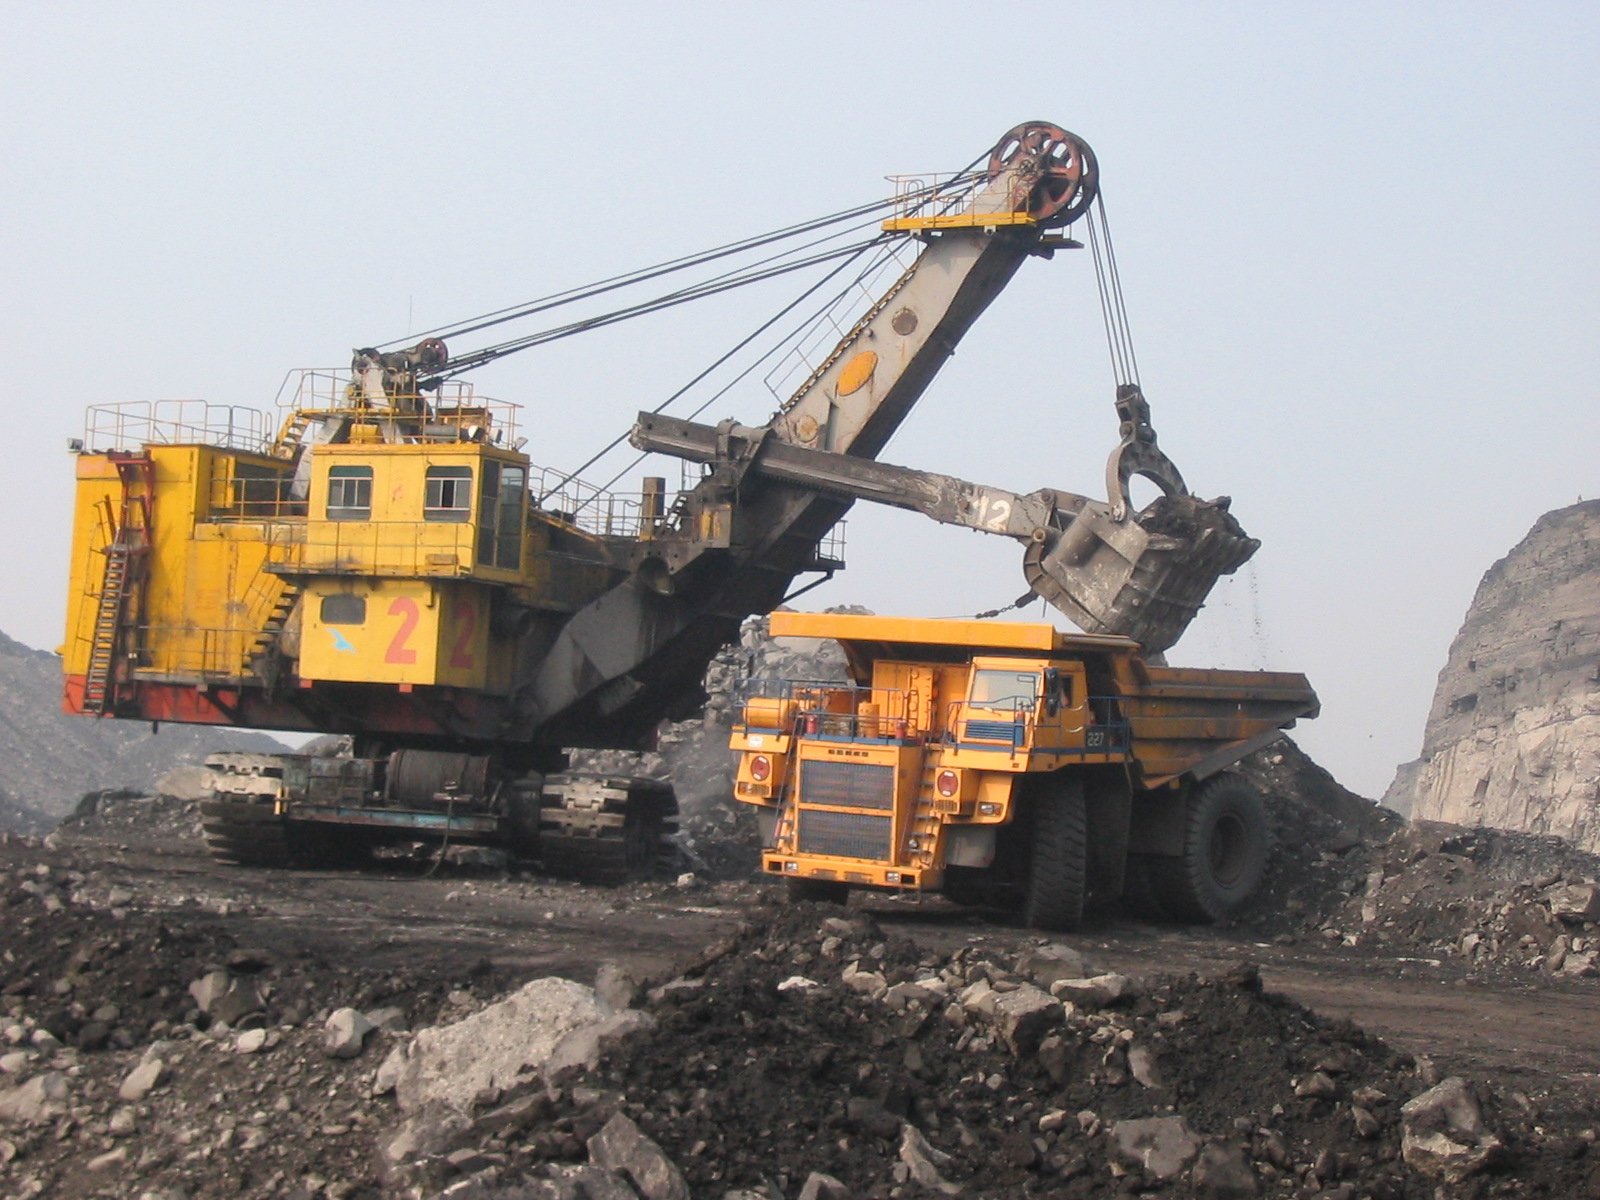
\includegraphics[width=.6\linewidth]{img/Excavator} \\
		\tiny{originally posted to Flickr by FAndrey at http://flickr.com/photos/43301444@N06/4141786255}
	\end{figure}

	\begin{itemize}
		\item{Goal: \textbf{Optimization of model parameters}}
		\item{Models of technical system = Physical properties + Control properties}
	\end{itemize}
\end{frame}

\begin{frame}
	\frametitle{Problem Setting: Schematic Illustration}
	\begin{figure}[bth]
		\centering
		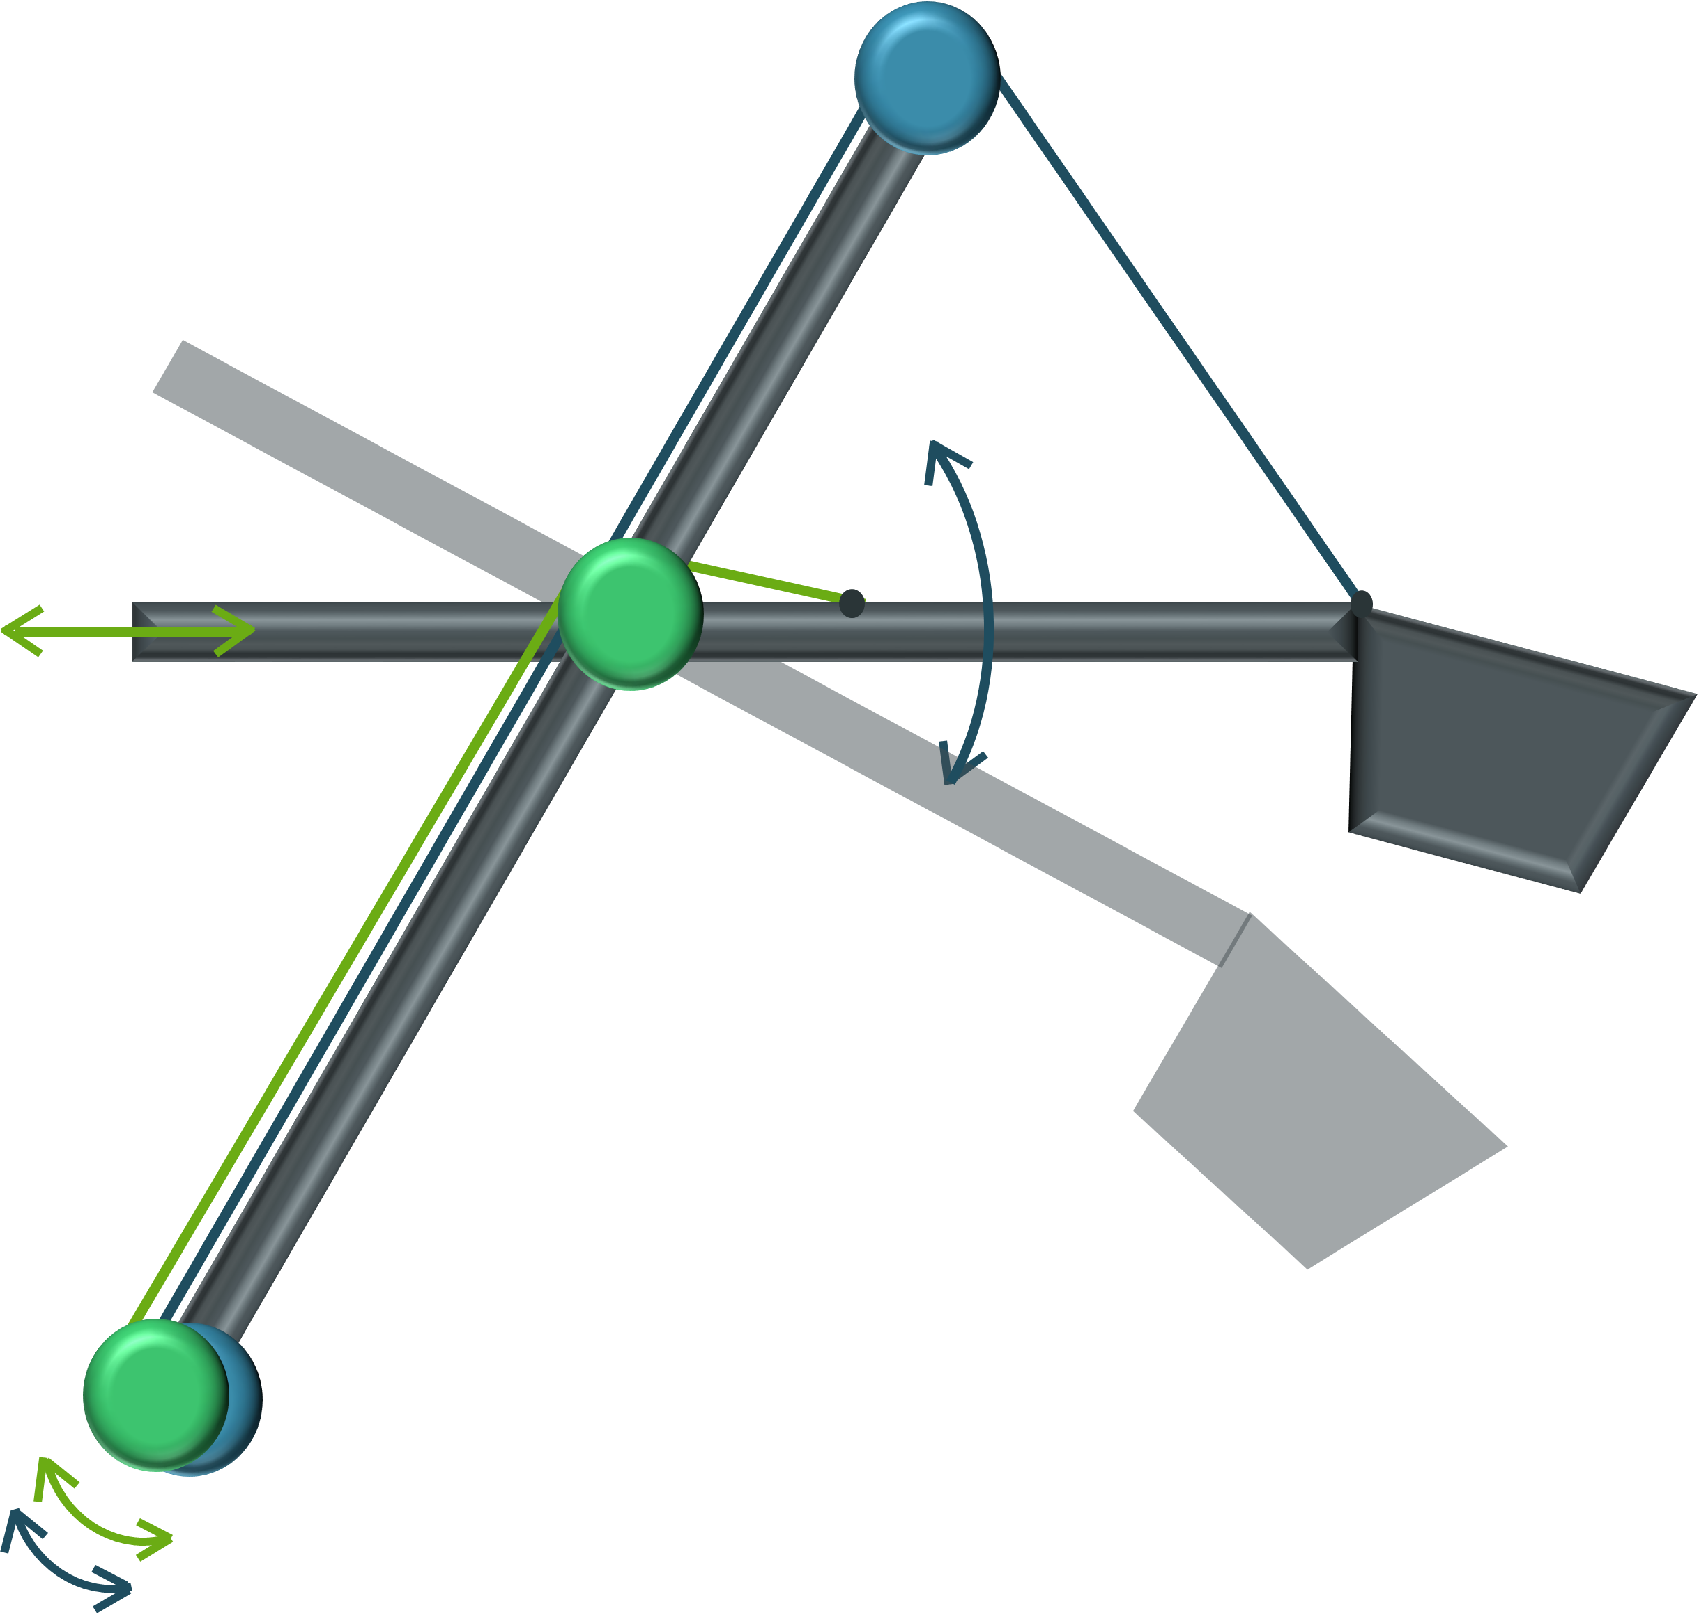
\includegraphics[width=.5\linewidth]{img/Problem_1}
	\end{figure}
\end{frame}

%\begin{frame}
%	\frametitle{Problem Setting}
%	\begin{figure}[bth]
%		\centering
%		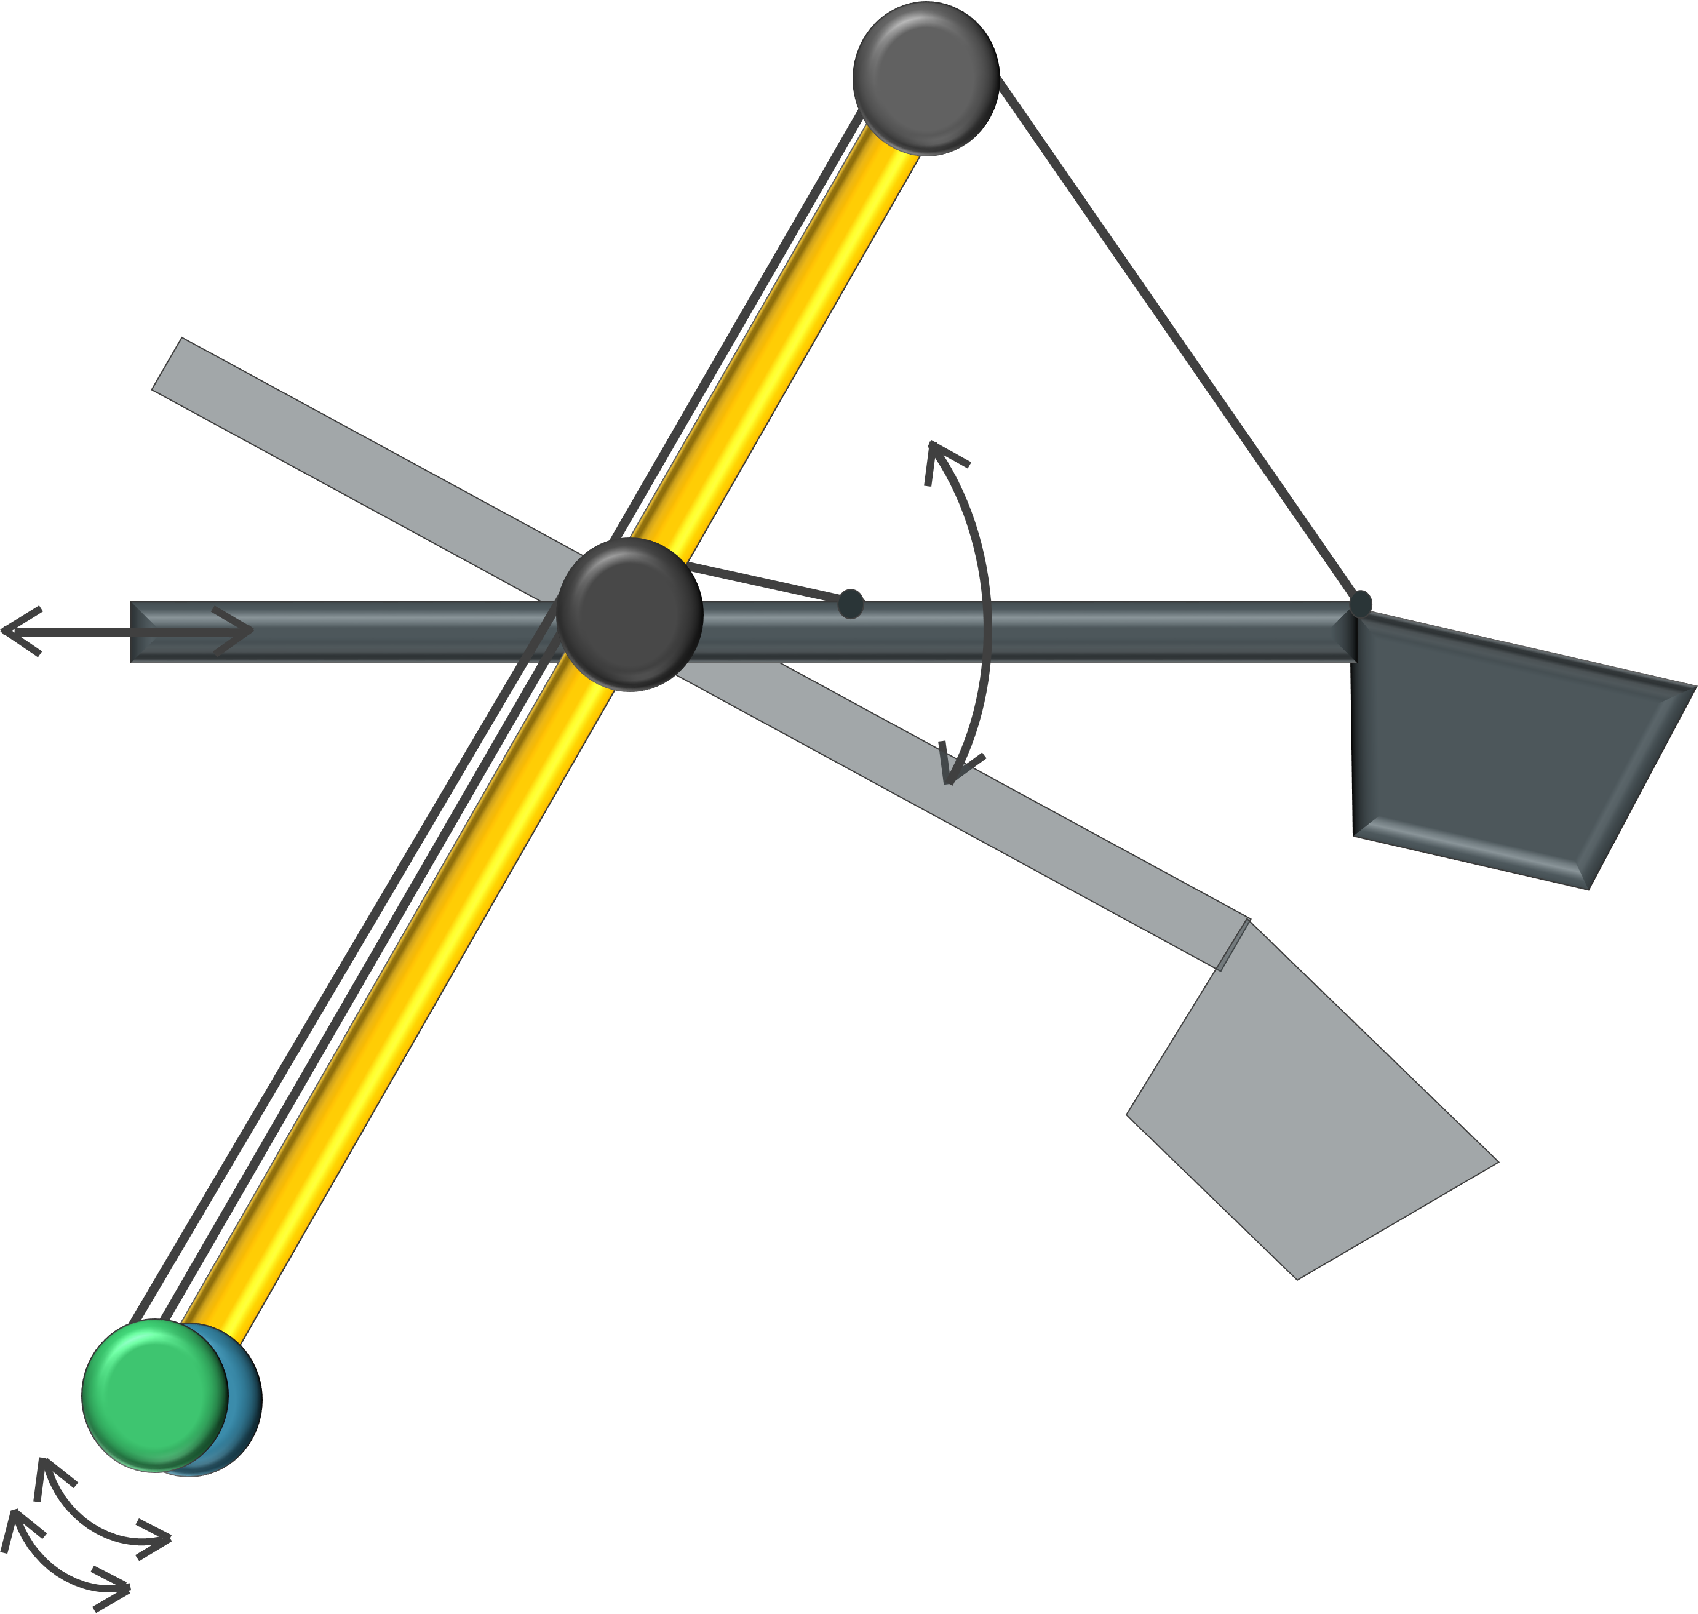
\includegraphics[width=.4\linewidth]{img/Problem_2}
%	\end{figure}
%	\begin{itemize}
%		\item{Arm element fixed to the base}
%		\item{Cannot be moved w.r.t. the base}
%	\end{itemize}
%\end{frame}

%\begin{frame}
%	\frametitle{Problem Setting (include videos)}
%	\begin{figure}[bth]
%		\centering
%		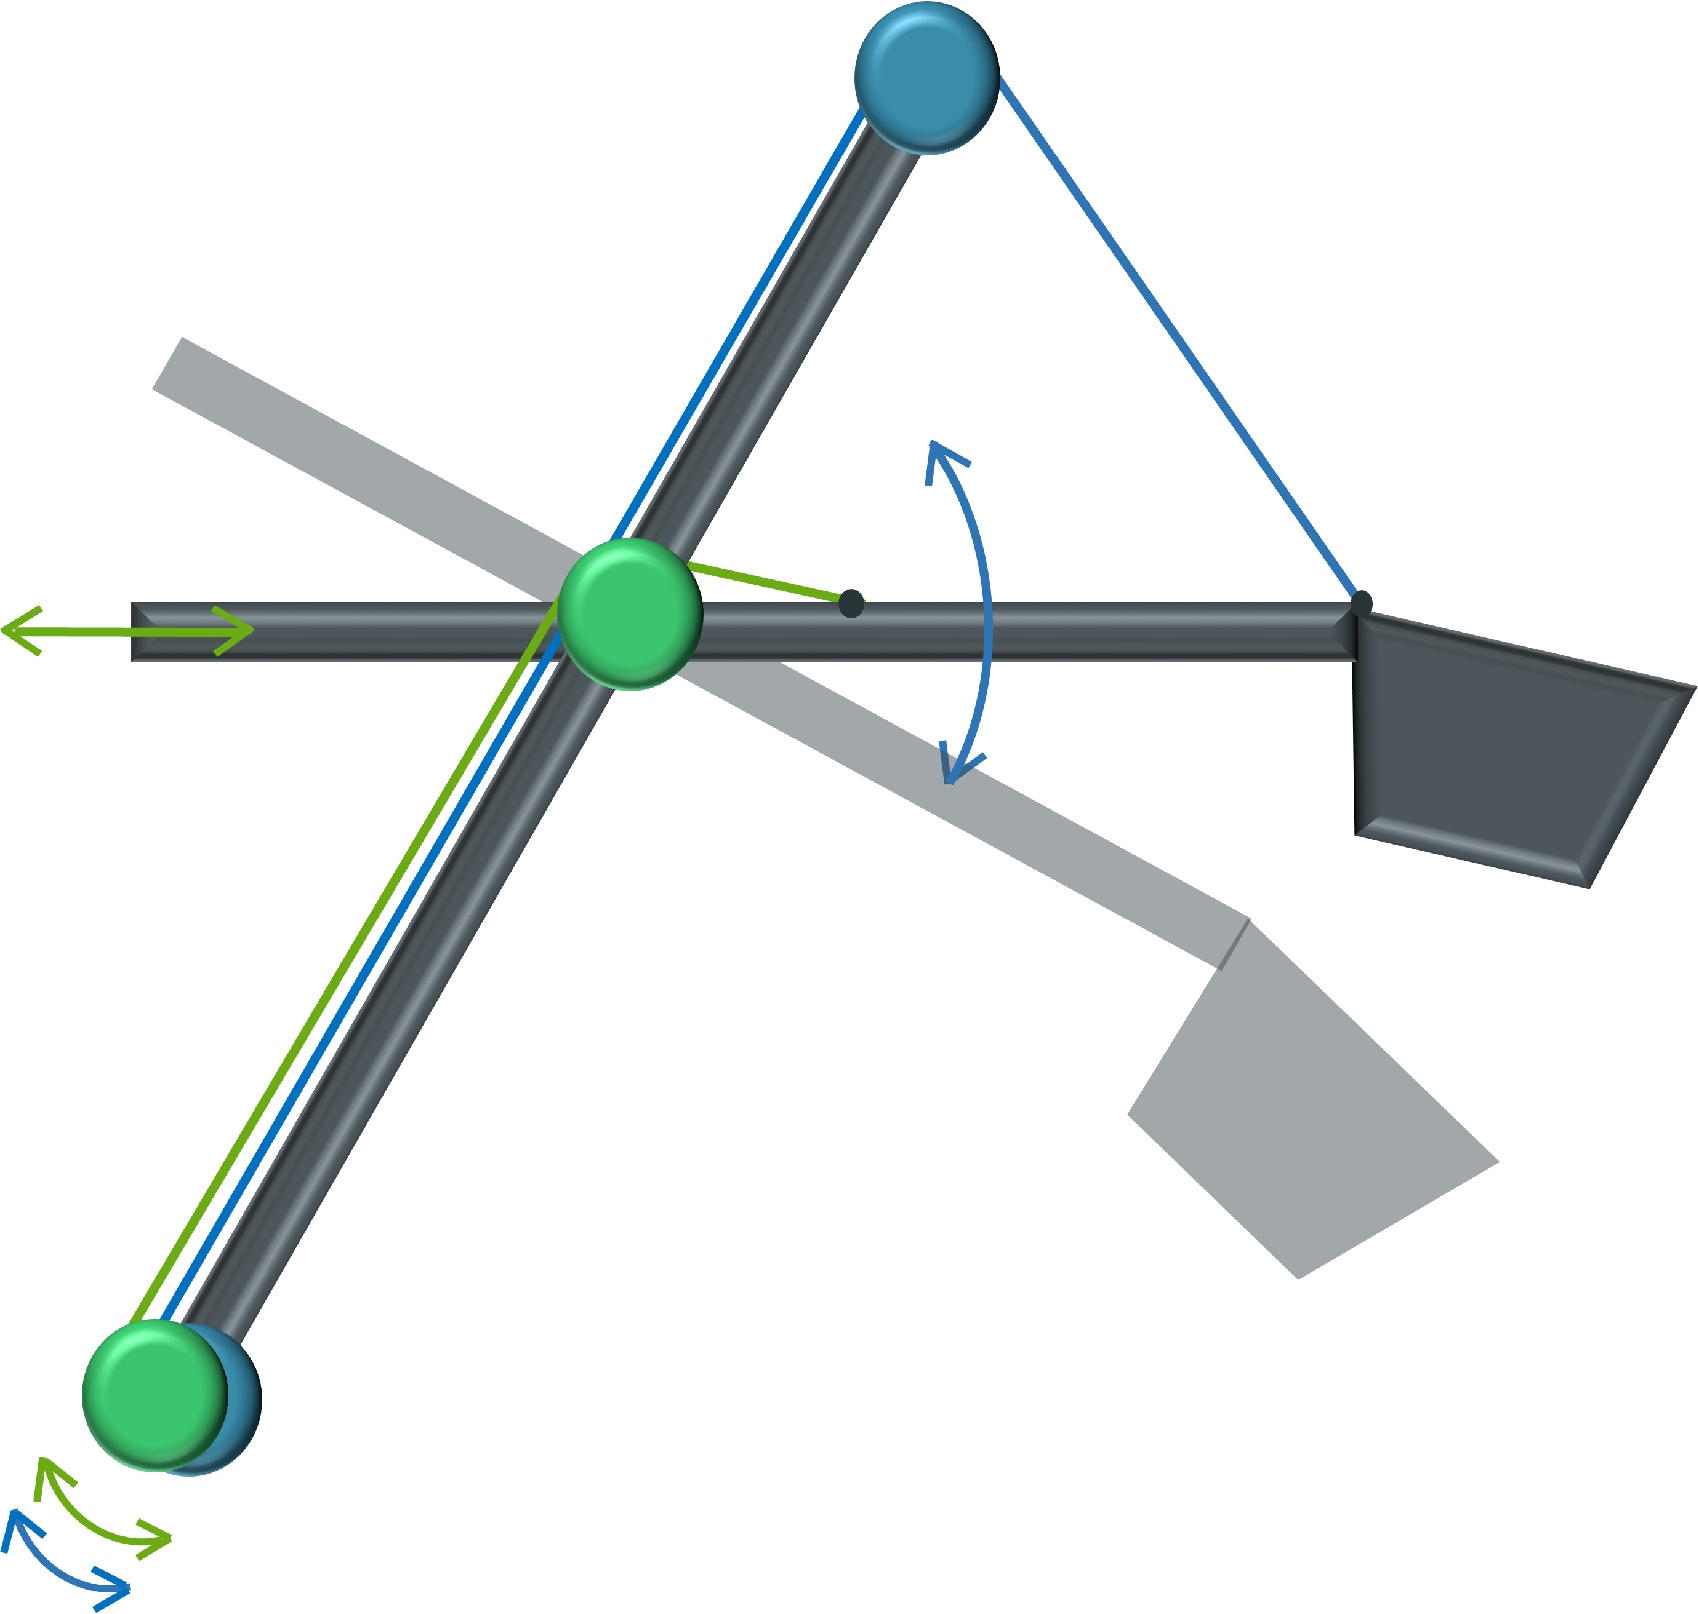
\includegraphics[width=.4\linewidth]{img/Problem_3}
%	\end{figure}
%	\centering
%	\begin{itemize}
%		\item{\makebox[1.5cm][l]{\textcolor[rgb]{0,0.69,0.32}{Green:}} Shovel motion \textbf{back} and \textbf{forth}}
%		\item{\makebox[1.5cm][l]{\textcolor[rgb]{0.18,0.46,0.71}{Blue:}} Shovel motion \textbf{up} and \textbf{down}} \\
%	\end{itemize}
%\end{frame}

\begin{frame}
	\frametitle{Problem Setting}
\centering
\includemedia[
  label      = AA,
  width      = 80mm,
  height     = 50mm,
  activate   = pageopen,
  addresource= videos/ArmMovement.mp4,
  flashvars={flv=videos/ArmMovement.mp4 & autoplay=1 & loop=1}
]{}{player_flv_maxi.swf}
\end{frame}





\begin{frame}
    \frametitle{Procedure}
    \onslide<1->
    \begin{columns}[onlytextwidth]
        \begin{column}{0.4\textwidth}
            \begin{block}{\centering{Physical Model}}
                \begin{itemize}
                    \item{Rope properties}
                    \item{Lagrange Formalism}
                \end{itemize}
            \end{block}
            
            \centering
            $\Downarrow$

            
            \begin{block}{\centering{Parameter Identification}}
            \centering{Discretization + Optimization}
            \end{block}
        \end{column}
        
    \onslide<2>
        
        \begin{column}{0.065\textwidth}
        \textbf{and}
        \end{column}
        
        \begin{column}{0.4\textwidth}
            \begin{exampleblock}{\centering{Blackbox Model}}
                \begin{itemize}
                    \item{Realistic model}
                    \item{Confidential information}
                \end{itemize}
            \end{exampleblock}
            
            \centering
            $\Downarrow$
            
            \begin{exampleblock}{\centering{Parameter Identification}}
            \centering{Derivative-free optimization}
            \end{exampleblock}
        \end{column}
    \end{columns}
\end{frame}





\begin{frame}
\setbeamertemplate{blocks}[rounded][shadow=false]
    \frametitle{Physical Modeling}
    \vspace{0.3cm}
		\large\textbf{Why?}
		\vspace{1cm}
		\begin{columns}
			\column{.3\textwidth}
				\centering
		    	\begin{block}{}
		    	    \begin{center}
		    	    \vskip 4mm
					{\large Building an accurate model}
					\vskip 3mm
					\hspace*\fill
					\end{center}
				\end{block}
			\column{.1\textwidth}
				\centering
				\Huge{$\Rightarrow$}
			\column{.3\textwidth}
				\centering
				\begin{block}{}
				    \begin{center}
				    \vskip 2mm
					Good description of the effects of control and motion
					%\vskip
					\hspace*\fill
					\end{center}
				\end{block}
		\end{columns}
	\vspace{0.5cm}
\end{frame}
	
	
\begin{frame}
    \frametitle{Physical Modeling Cont'd}
    \vspace{-0.3cm}
    \large\textbf{How?}
    \vspace{1cm}
	    \begin{columns}
	    \column{0.45\textwidth}
	    \onslide<1->
		To consider:
		\vspace{0.25cm}
		\begin{itemize}
			\item{Friction in cable reels}
			\item{Potential/Kinetic energy}
			\item{etc}
		\end{itemize}
		
		\onslide<2>
		\column{0.1\textwidth}
		    \Huge{$\rightarrow$}
		\column{0.35\textwidth}
		\large\textcolor{red}{Lagrange Formalism}\newline
		\centering{(ODE)}
	\end{columns}
\end{frame}


\begin{frame}
	\frametitle{Which color do we want to use?}
	\begin{tcolorbox}[width=\linewidth,colback={TUMblue}]
		TUMblue
	\end{tcolorbox}
	\begin{tcolorbox}[width=\linewidth,colback={TUMblue1}]
		TUMblue1
	\end{tcolorbox}
	\begin{tcolorbox}[width=\linewidth,colback={TUMblue2}]
		TUMblue2
	\end{tcolorbox}
	\begin{tcolorbox}[width=\linewidth,colback={TUMblue3}]
		TUMblue3
	\end{tcolorbox}
	\begin{tcolorbox}[width=\linewidth,colback={TUMblue4}]
		TUMblue4
	\end{tcolorbox}
	\begin{tcolorbox}[width=\linewidth,colback={TUMblue5}]
		TUMblue5
	\end{tcolorbox}
\end{frame}











\begin{frame}
\setbeamertemplate{blocks}[rounded][shadow=false]
	\frametitle{Parameter Identification}
	\onslide<1->
		\large\textbf{What are parameters?}
		\vspace{0.2cm}
		\begin{itemize}
			\item{Friction coefficients}
			\item{Mass}
			\item{Inertia}
		\end{itemize}
	\vspace{0.5cm}
	\onslide<2>
		\large\textbf{Why?}
		\begin{columns}
			\column{.3\textwidth}
				\centering
		    	\begin{block}{}
		    	    \begin{center}
		    	    \vskip 4mm
					 Accurate and realistic parameters
					\vskip 3mm
					\hspace*\fill
					\end{center}
				\end{block}
			\column{.1\textwidth}
				\centering
				\Huge{$\Rightarrow$}
			\column{.3\textwidth}
				\centering
				\begin{block}{}
				    \begin{center}
				    \vskip 2mm
					Better prediction and planning of motion
					%\vskip
					\hspace*\fill
					\end{center}
				\end{block}
		\end{columns}
	\vspace{0.5cm}
\end{frame}
		


   


		
		
\begin{frame}
    \frametitle{Parameter Identification Two Ways}
%    \vspace{0.2cm}
    \textbf{Two independent models acquired,}\newline
    \textbf{two different computational approaches.}
    \vspace{1cm}
    \begin{columns}[onlytextwidth]
        \begin{column}{0.4\textwidth}
            \begin{block}{\centering{Physical Model}}
%                \begin{itemize}
%                   \item{Rope properties}
%                    \item{Lagrange Formalism}
%                \end{itemize}
            \end{block}
            
            \centering
            $\Downarrow$
            
            \begin{block}{\centering{Parameter Identification}}
%            \centering{Discretization}
            \end{block}
        \end{column}
        
        \begin{column}{0.065\textwidth}
        \textbf{and}
        \end{column}
        
        \begin{column}{0.4\textwidth}
            \begin{exampleblock}{\centering{Blackbox Model}}
%                \begin{itemize}
%                    \item{Realistic model}
%                    \item{Confidential information}
%                \end{itemize}
            \end{exampleblock}
            
            \centering
            $\Downarrow$
            
            \begin{exampleblock}{\centering{Parameter Identification}}
%            \centering{Derivative-free optimization}
            \end{exampleblock}
        \end{column}
    \end{columns}
\end{frame}		
		

\begin{frame}
    \frametitle{Parameter Identification: Physical Model}
    \vspace{-1cm}
    \onslide<1->
    \begin{columns}[onlytextwidth]
        \begin{column}{0.5\textwidth}
            \begin{block}{\centering{Own Physical Model}}
                
                    \centering{Lagrange Formalism}
%                    \small{{\begin{align*}
%	                        &A(x,p)
%	                \begin{pmatrix} 
%	                \ddot{s} \\ \ddot{\theta} \\
%	                \end{pmatrix}
%	                = b(x,u,p)
%                   \end{align*}}}
%            \vspace{-0.3cm}   
            \end{block}
            \vspace{-0.1cm}
            
            \centering
            $\Downarrow$
            
            \begin{block}{\centering{Parameter Identification}}
            Discretization
            \small{\begin{align*}
                \min_{p} & & \frac{1}{2} \| \bar{x} - x(p) \|^2 & & \\
            \end{align*}}
            \vspace{-1cm}
            \end{block}
            \vspace{-1.5cm}
        \end{column}
    
    \onslide<2>
    \begin{column}{0.45\textwidth}
        \begin{itemize}
            \vspace{0.6cm}
            \item{Information for calibration available}
            \vspace{0.5cm}
            \item{Runge-Kutta method}
            \vspace{0.5cm}
            \item{Parameter computation for}\newline{a given control and motion}
        \end{itemize}
    \end{column}    
    \end{columns}
\end{frame}        
        
        
        
        
        
        
        
        
\begin{frame}        
    \frametitle{Parameter Identification: Blackbox Model}
    
    \onslide<2>
    \begin{columns}[onlytextwidth]
        \begin{column}{0.5\textwidth}
        \begin{itemize}
        	\vspace{-1.5cm}
            \item{Almost no information available}
            \vspace{0.65cm}
            \item{Derivative-free optimization}
            \vspace{0.65cm}
            \item{Only a few parameters studied}
        \end{itemize}
        \end{column}
    
    
    
    \onslide<1->
    \begin{column}{0.45\textwidth}
            \begin{exampleblock}{\centering{Siemens Blackbox Model}}
                \begin{itemize}
                
                \item{\textbf{Input}: Control}
                \item{\textbf{Output}: Motion}
                \end{itemize}
            \end{exampleblock}
            
            \centering
            $\Downarrow$
            
            \begin{exampleblock}{\centering{Parameter Identification}}
            Particle Swarm, Pattern Search, Genetic Algorithm, ...
            \end{exampleblock}
        \end{column}
      \end{columns}
\end{frame}



\begin{frame}
	\frametitle{Visualization: Simulink}
	\vspace{-5cm}
	\begin{figure}[t]
	\centering
		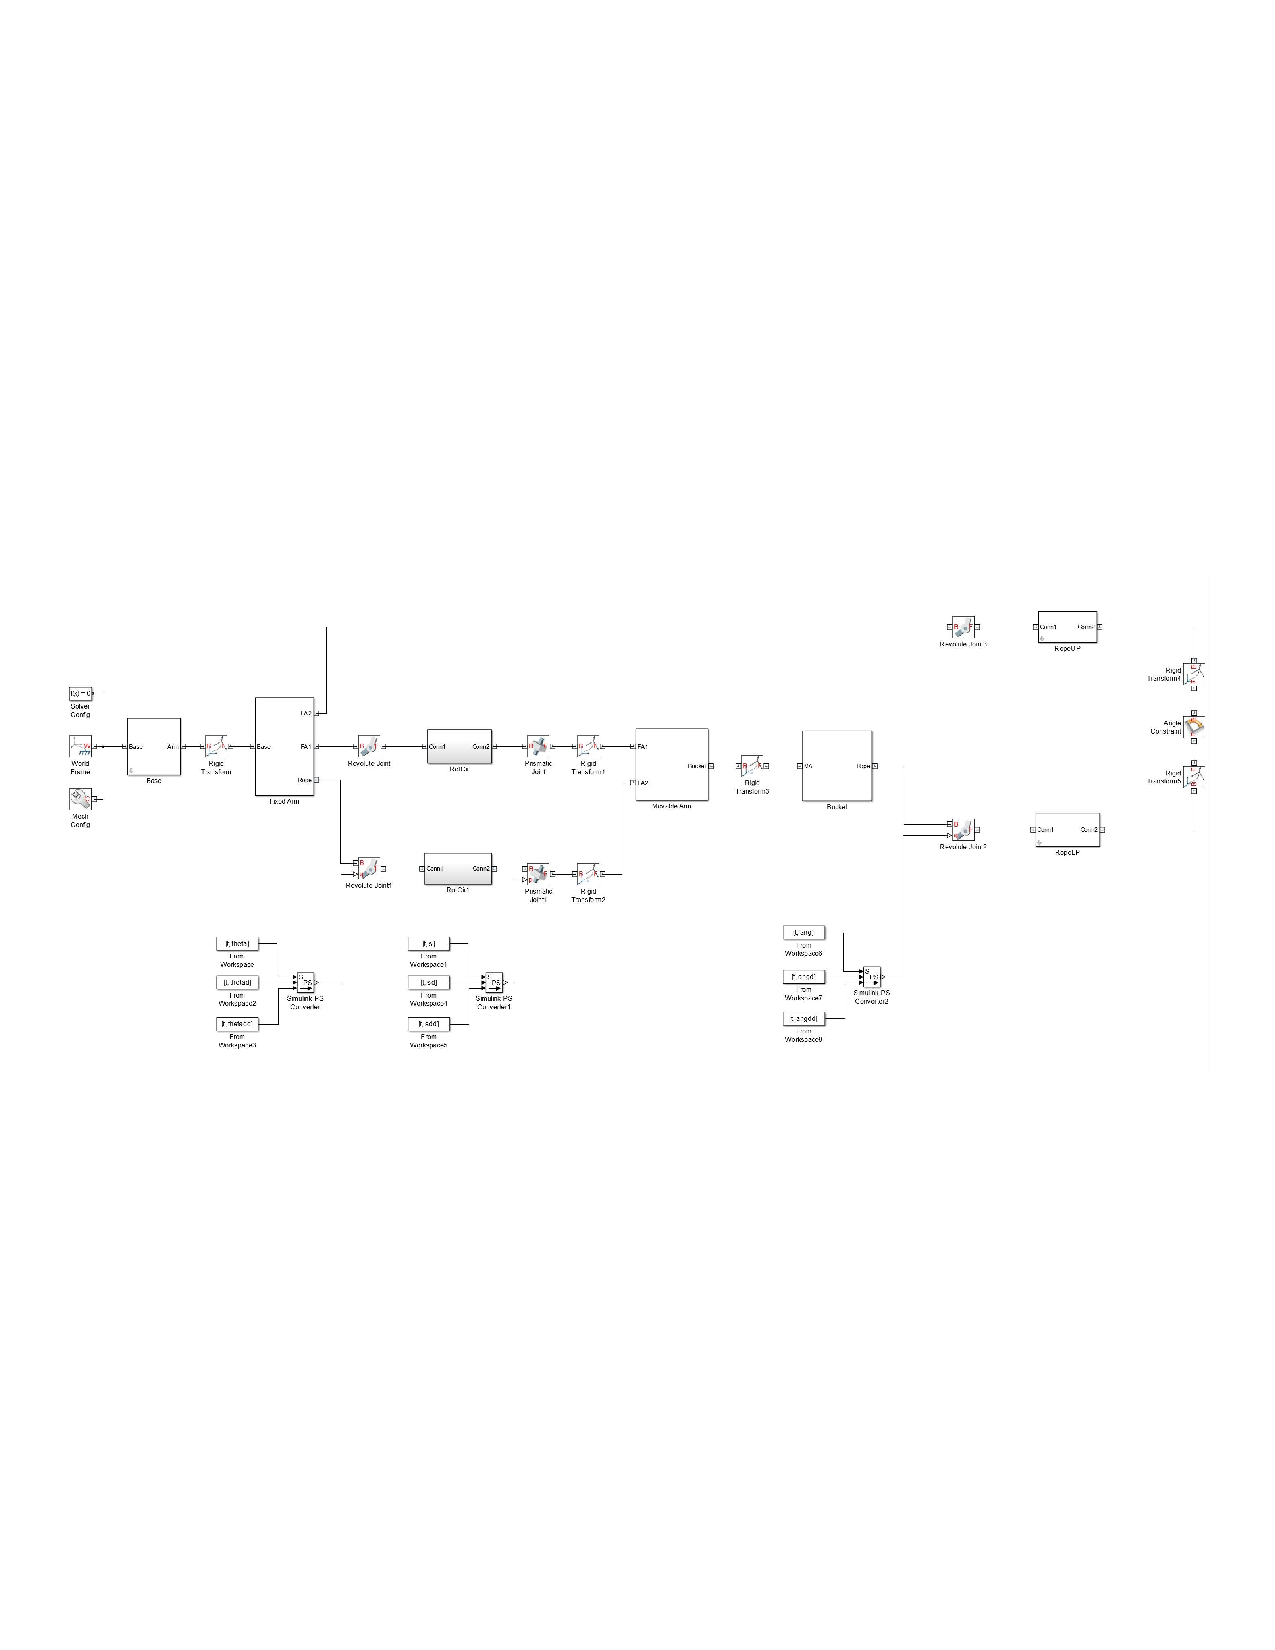
\includegraphics[width=1\linewidth, height=1.2\linewidth]{img/Simulink_Screenshot1}
	\end{figure}
	
	
\end{frame}







\begin{frame}[t]
\frametitle{Visualization Example}

Same parameters, different load weights
\vspace{0.5cm}

\begin{columns}
\begin{column}{0.45\textwidth}


\includemedia[
  label      = AA,
  width      = 50mm,
  height     = 50mm,
  activate   = pageopen,
  addresource= videos/traj_x_095p.mp4,
  flashvars={flv=videos/traj_x_095p.mp4 & autoplay=1 & loop=1}
]{}{player_flv_maxi.swf}
\end{column}


\begin{column}{0.055\textwidth}
	\textbf{vs}
\end{column}


\begin{column}{0.4\textwidth}
\includemedia[
  label      = BB,
  width      = 50mm,
  height     = 50mm,
  activate   = pageopen,
  addresource= videos/traj_x_105p.mp4,
  flashvars={flv=videos/traj_x_105p.mp4 & autoplay=1 & loop =1}
]{}{player_flv_maxi.swf}
\end{column}

\end{columns}

\end{frame}
   




\section{Physical Model}

\begin{frame}
	\frametitle{Lagrange Formalism}
	\onslide<1->
	Method to describe dynamics of an accelerated system\\
	\begin{small}
	\begin{tabular}{ll}
		 & \\
		T & kinetic energy\\
		V & potentials\\
		F & non-conservative external forces\\
		r & points of actions of forces F\\ %position vector
		q & free variables\\
		Q & generalized forces\\ \\
	\end{tabular}
	\end{small}
	
	\onslide<2>
	\begin{align*}
	&\frac{d}{dt}\left(\frac{\partial T}{\partial \dot{q}_i}\right) -
	\frac{\partial T}{\partial q_i} +
	\frac{\partial V}{\partial q_i}
	= Q_i \\
	& Q = \left(\frac{\partial r}{\partial q}\right)^T F\\
	\end{align*}
		
\end{frame}	

\begin{frame}
	\frametitle{Physical Model of Excavator}
	
	%left, bottom, right, top
	%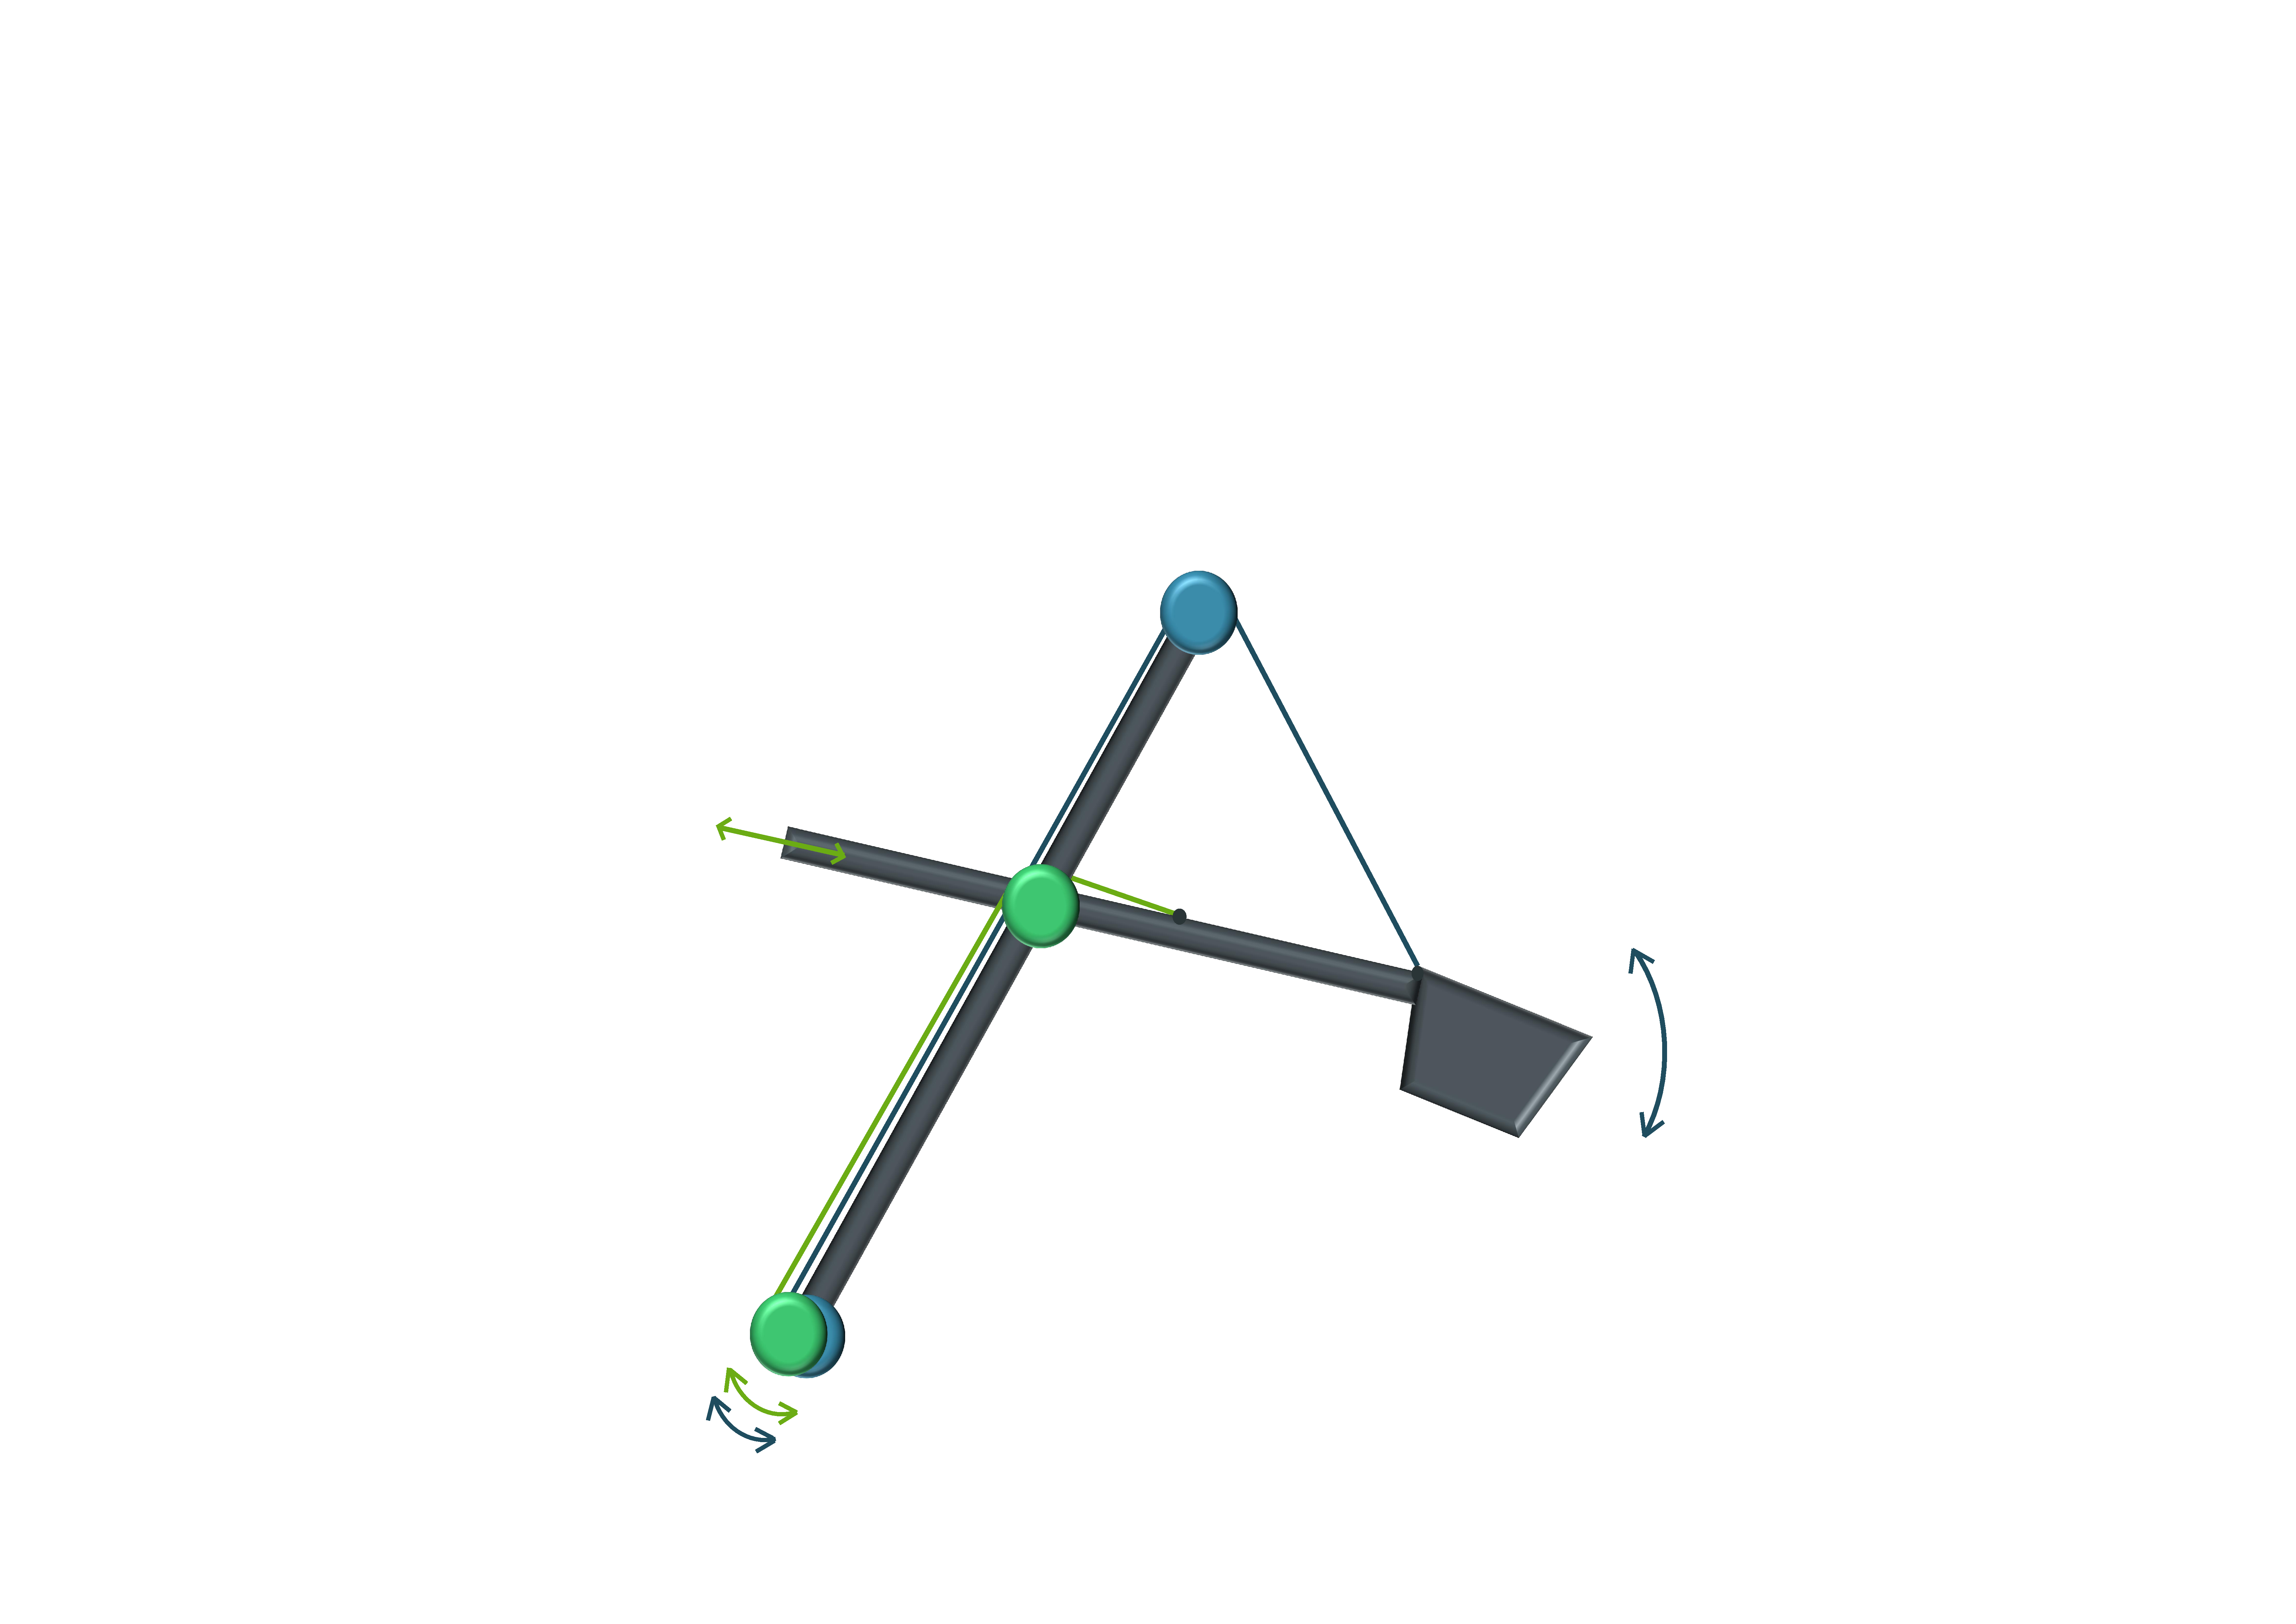
\includegraphics[trim=22cm 5cm 2cm 23cm, clip=true, width=\linewidth]{img/Excavator_Only}
	
	\begin{columns}
		\column{.6\linewidth}
			\centering
			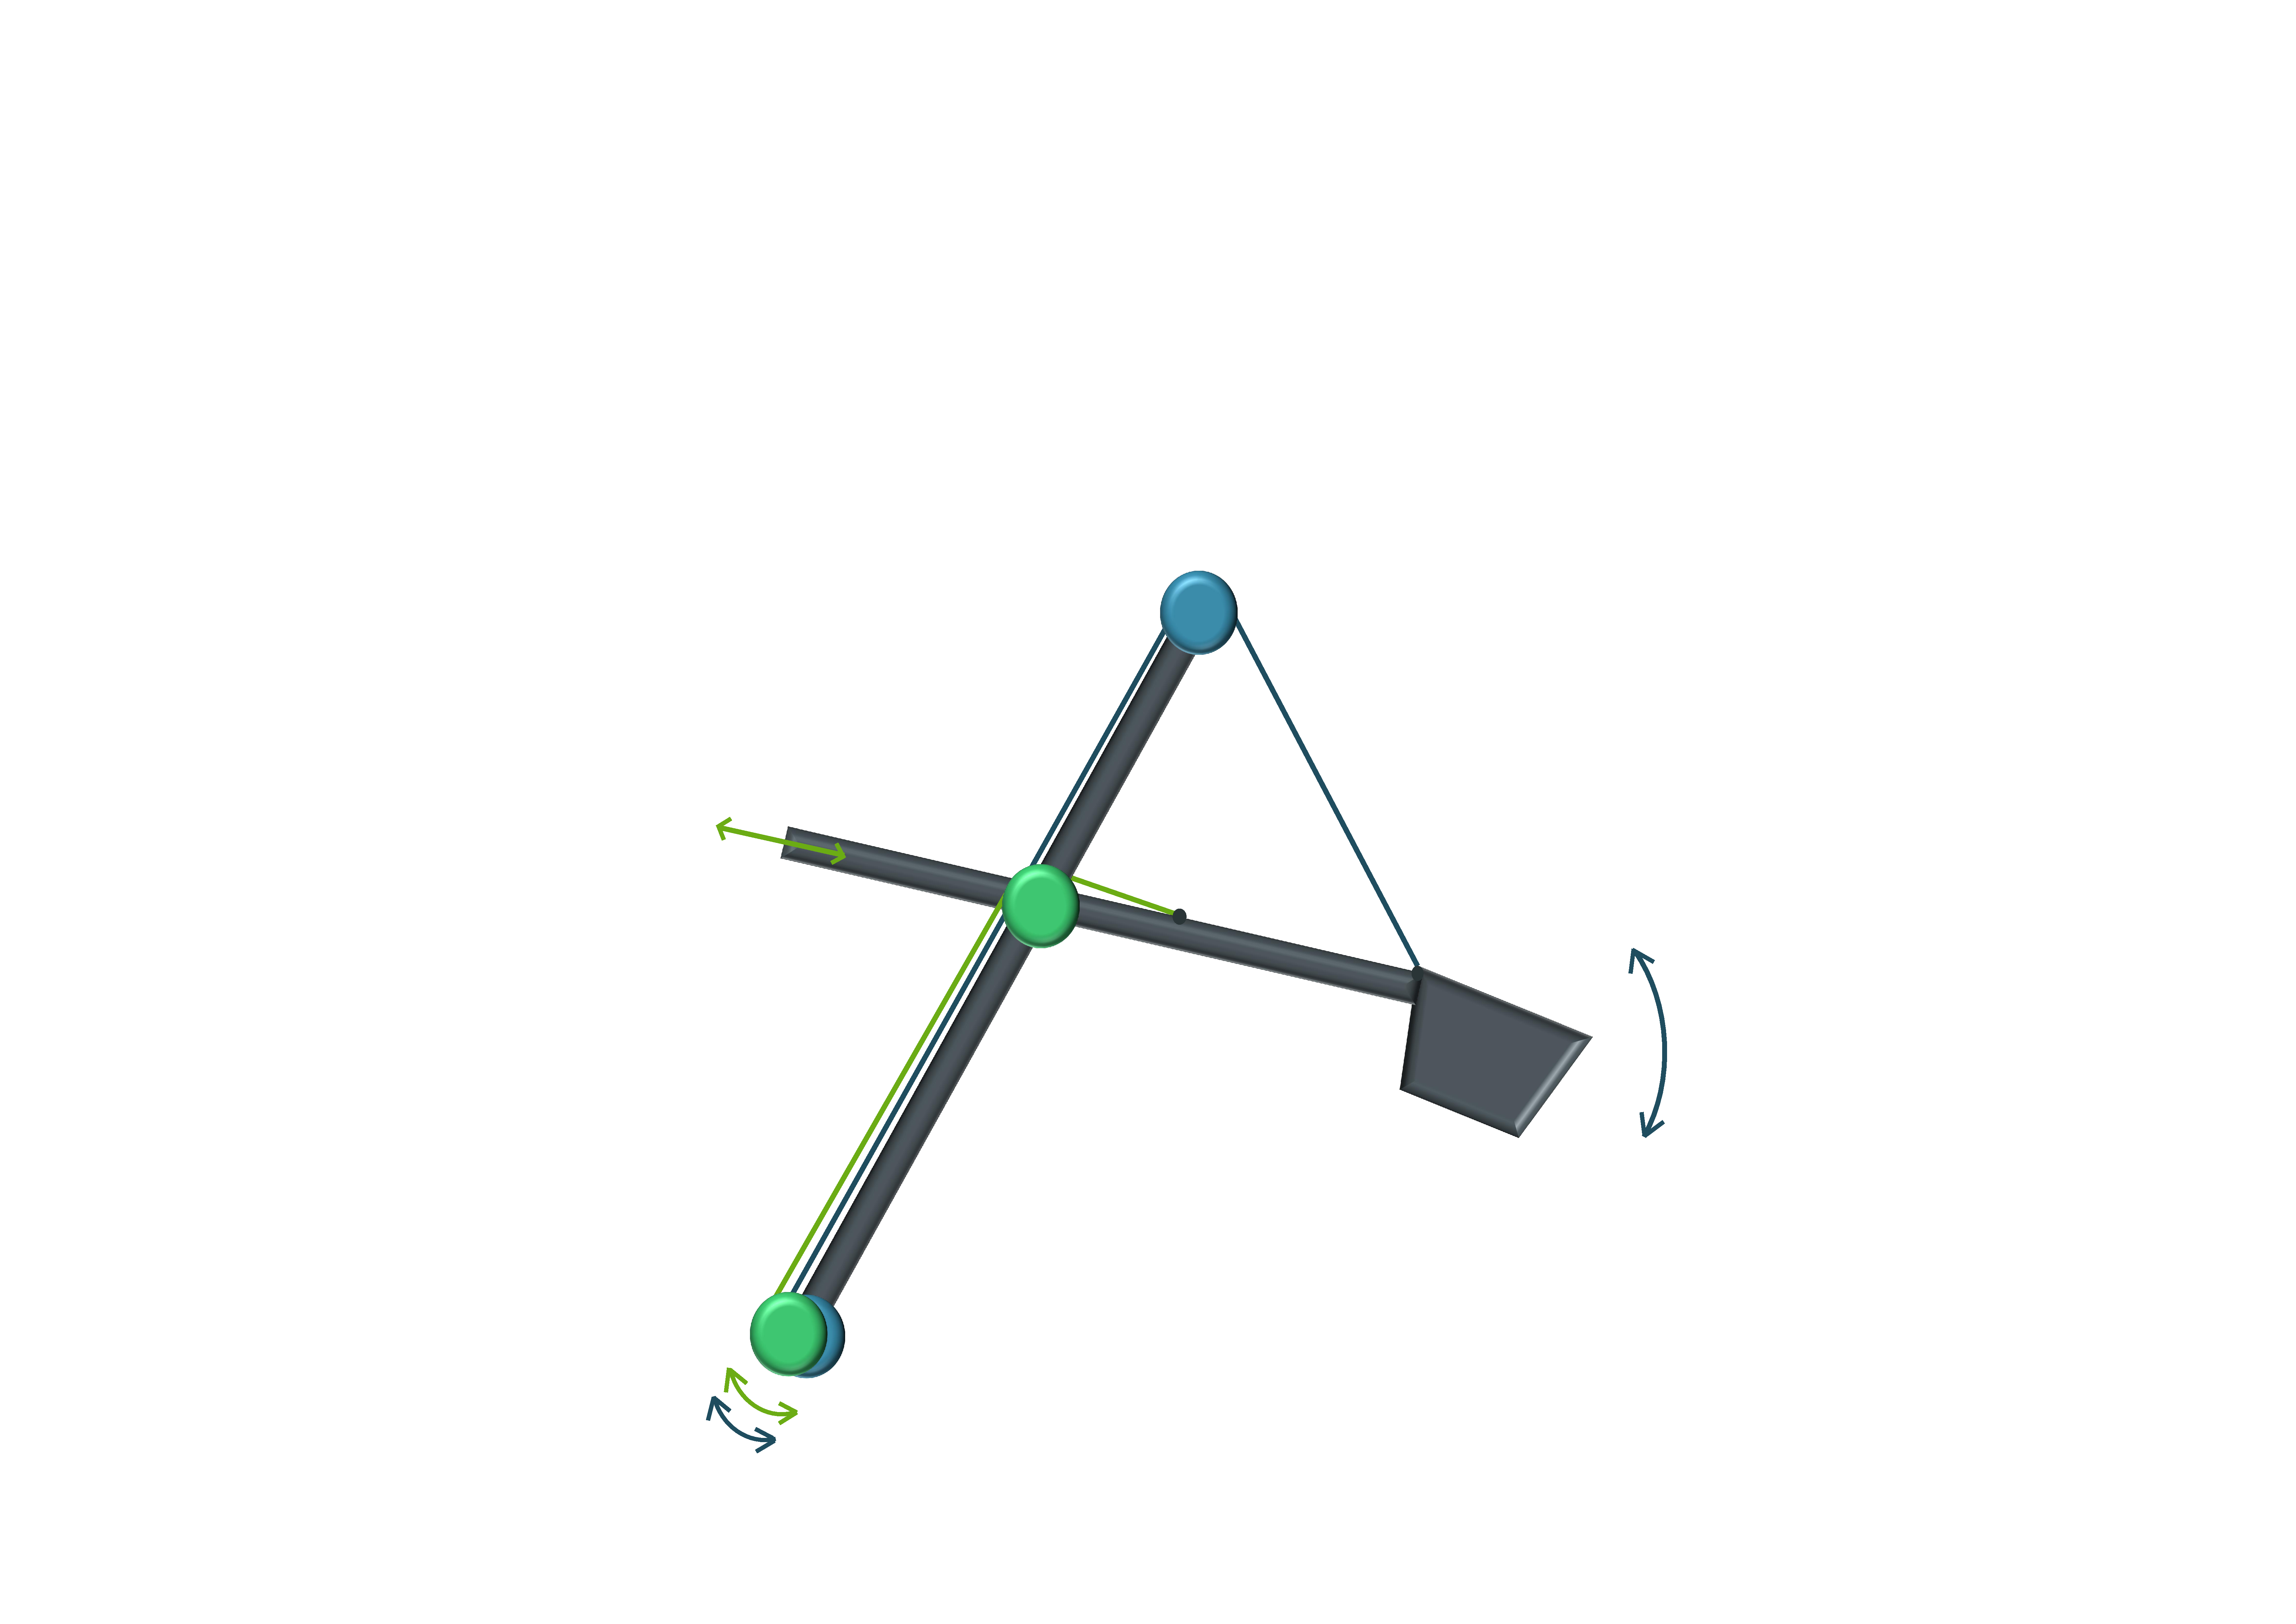
\includegraphics[trim=30cm 5cm 30cm 23cm, clip=true, width=\linewidth]{img/Excavator_Only}
		\column{.4\linewidth}
	\end{columns}
	
\end{frame}

\begin{frame}
	\frametitle{Physical Model of Excavator}
	
	%	invariant under transformation of coordinates $\rightarrow$ appropriate choice of 	coordinate system
	
	%first fix coordinate system $\rightarrow$ consider positions vectors, coordinates of mass points,... in this system\\
	
	%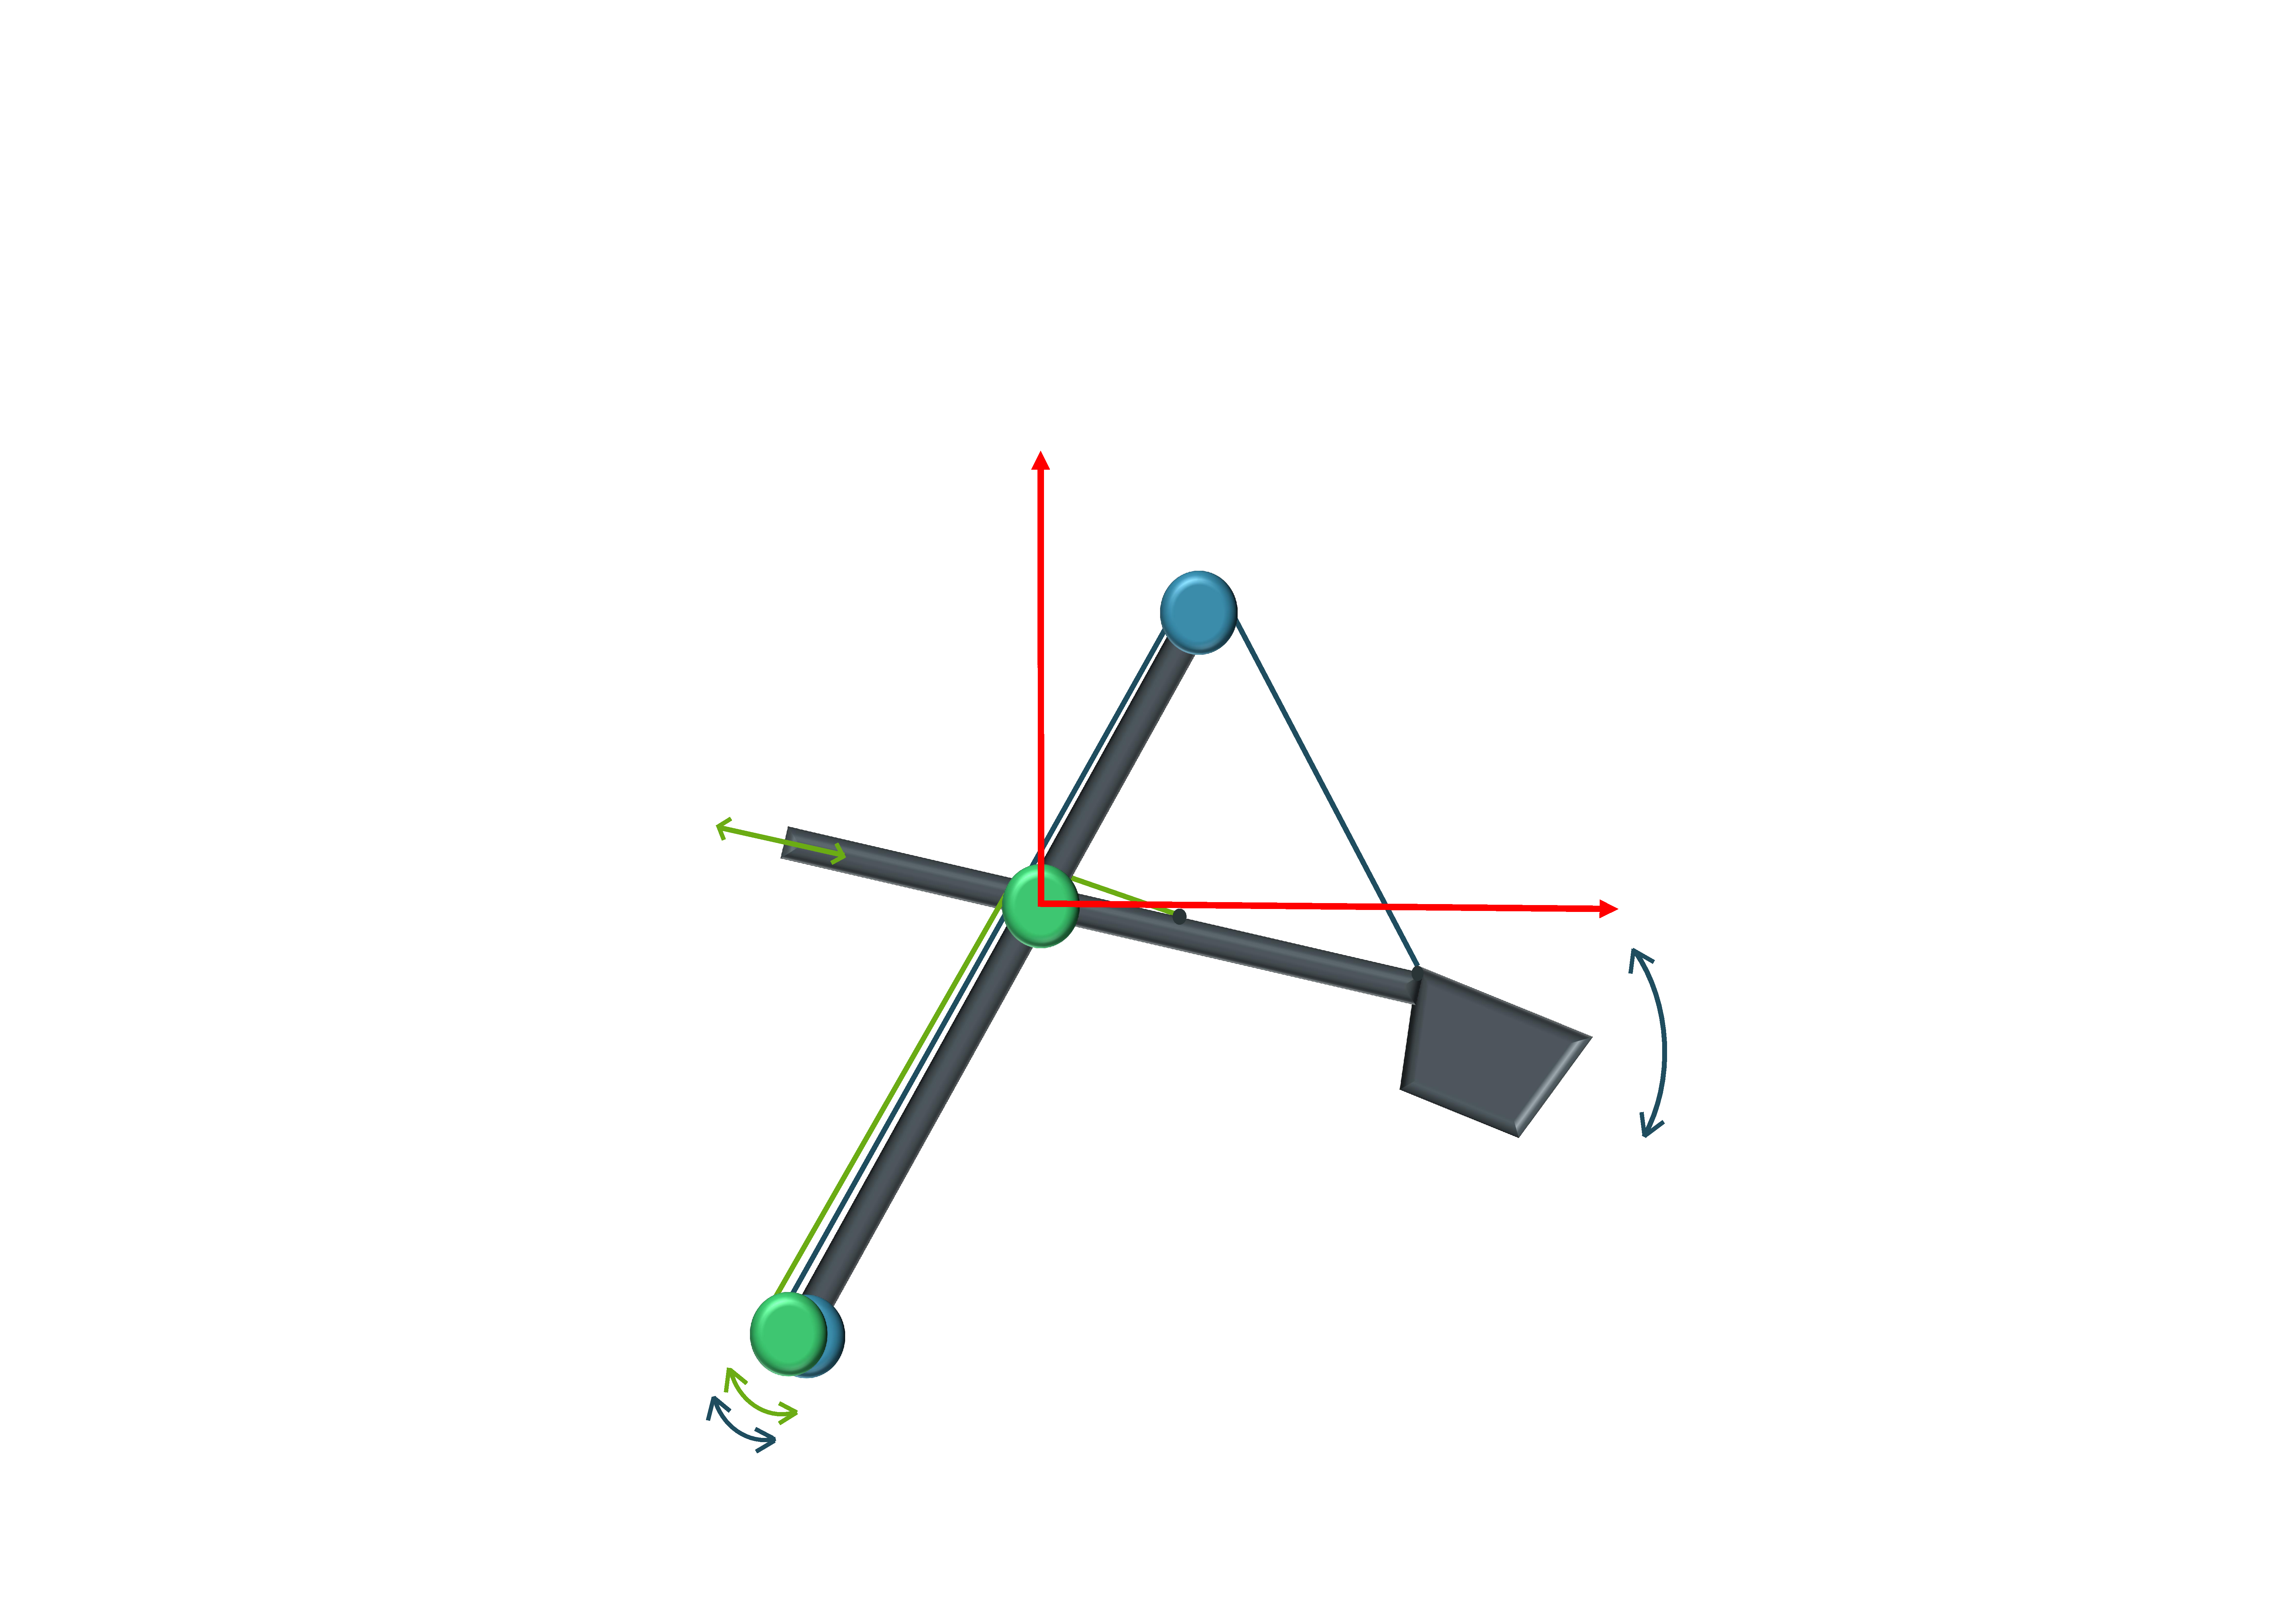
\includegraphics[trim=22cm 5cm 2cm 23cm, clip=true, width=\linewidth]{img/Excavator_coordinates2}
	
	\begin{columns}
		\column{.6\linewidth}
			\centering
			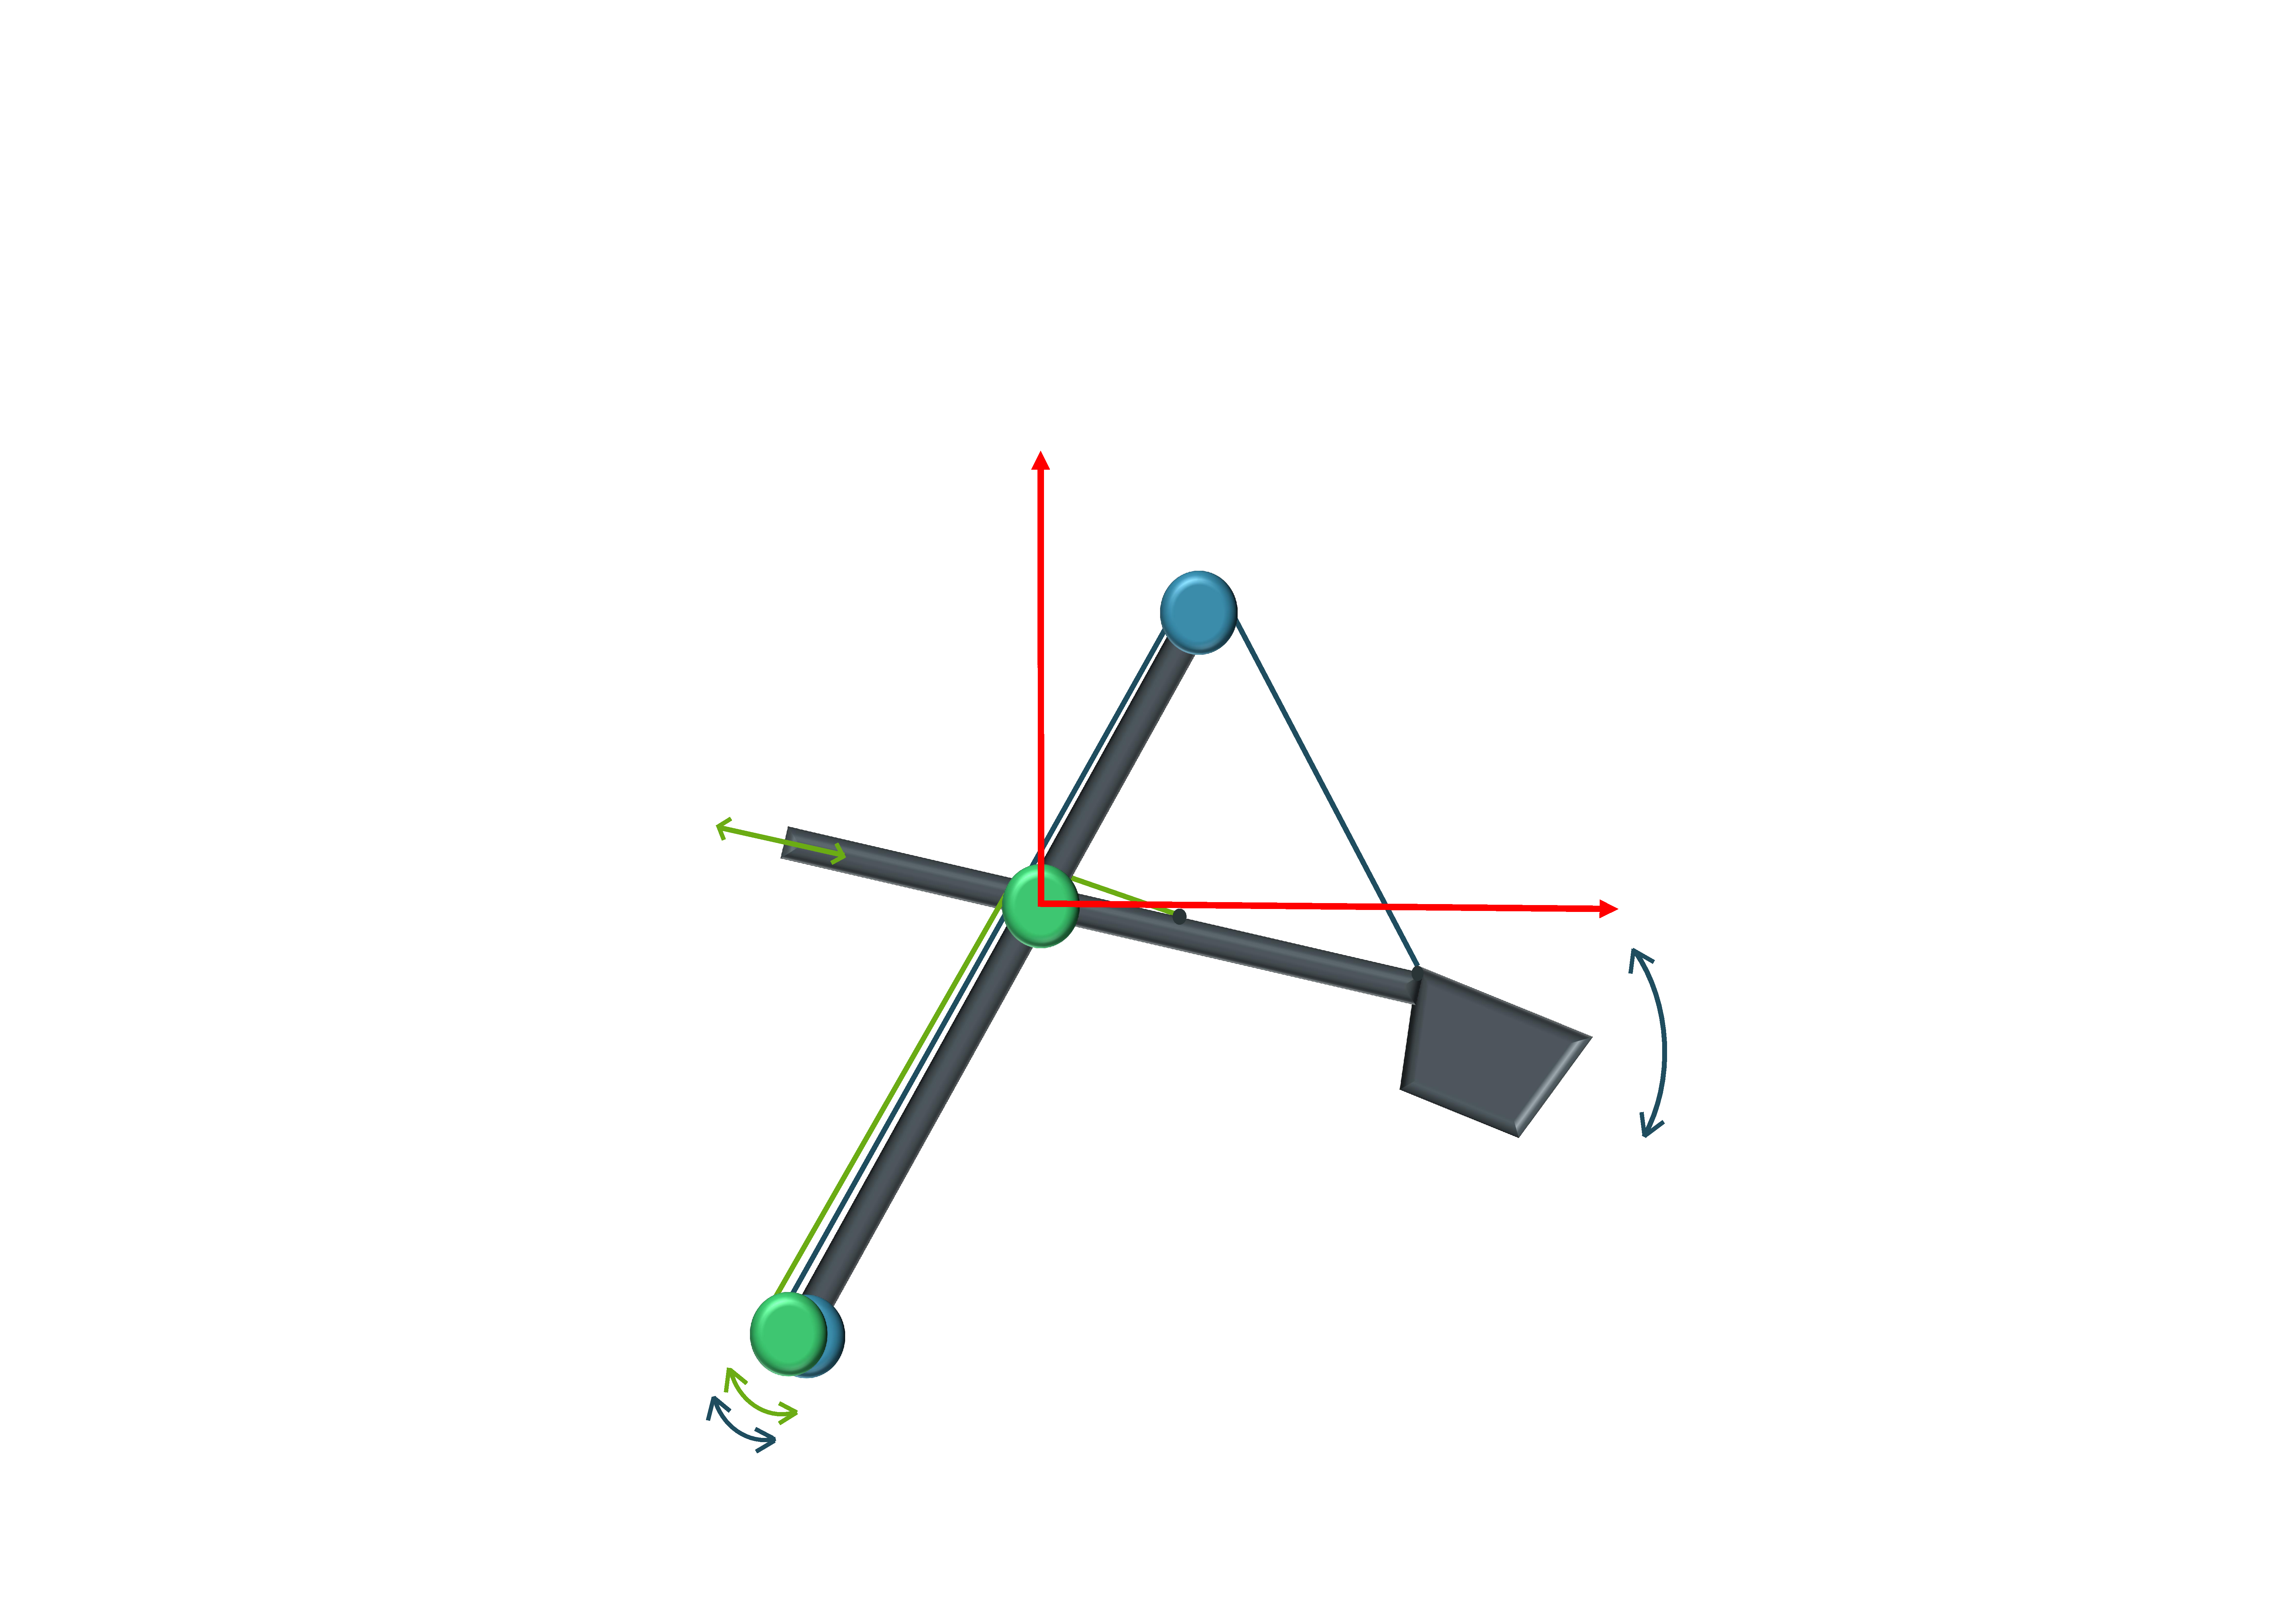
\includegraphics[trim=30cm 5cm 30cm 23cm, clip=true, width=\linewidth]{img/Excavator_coordinates2}
		\column{.4\linewidth}
			coordinate system
	\end{columns}
	
\end{frame}

\begin{frame}
	\frametitle{Physical Model of Excavator}
	
	%think of degrees of freedom $\rightarrow$ angle and length side arm $\rightarrow$ forces in the system will depend on excavator configuration and therefore on $s$ and $\theta$\\
	
	%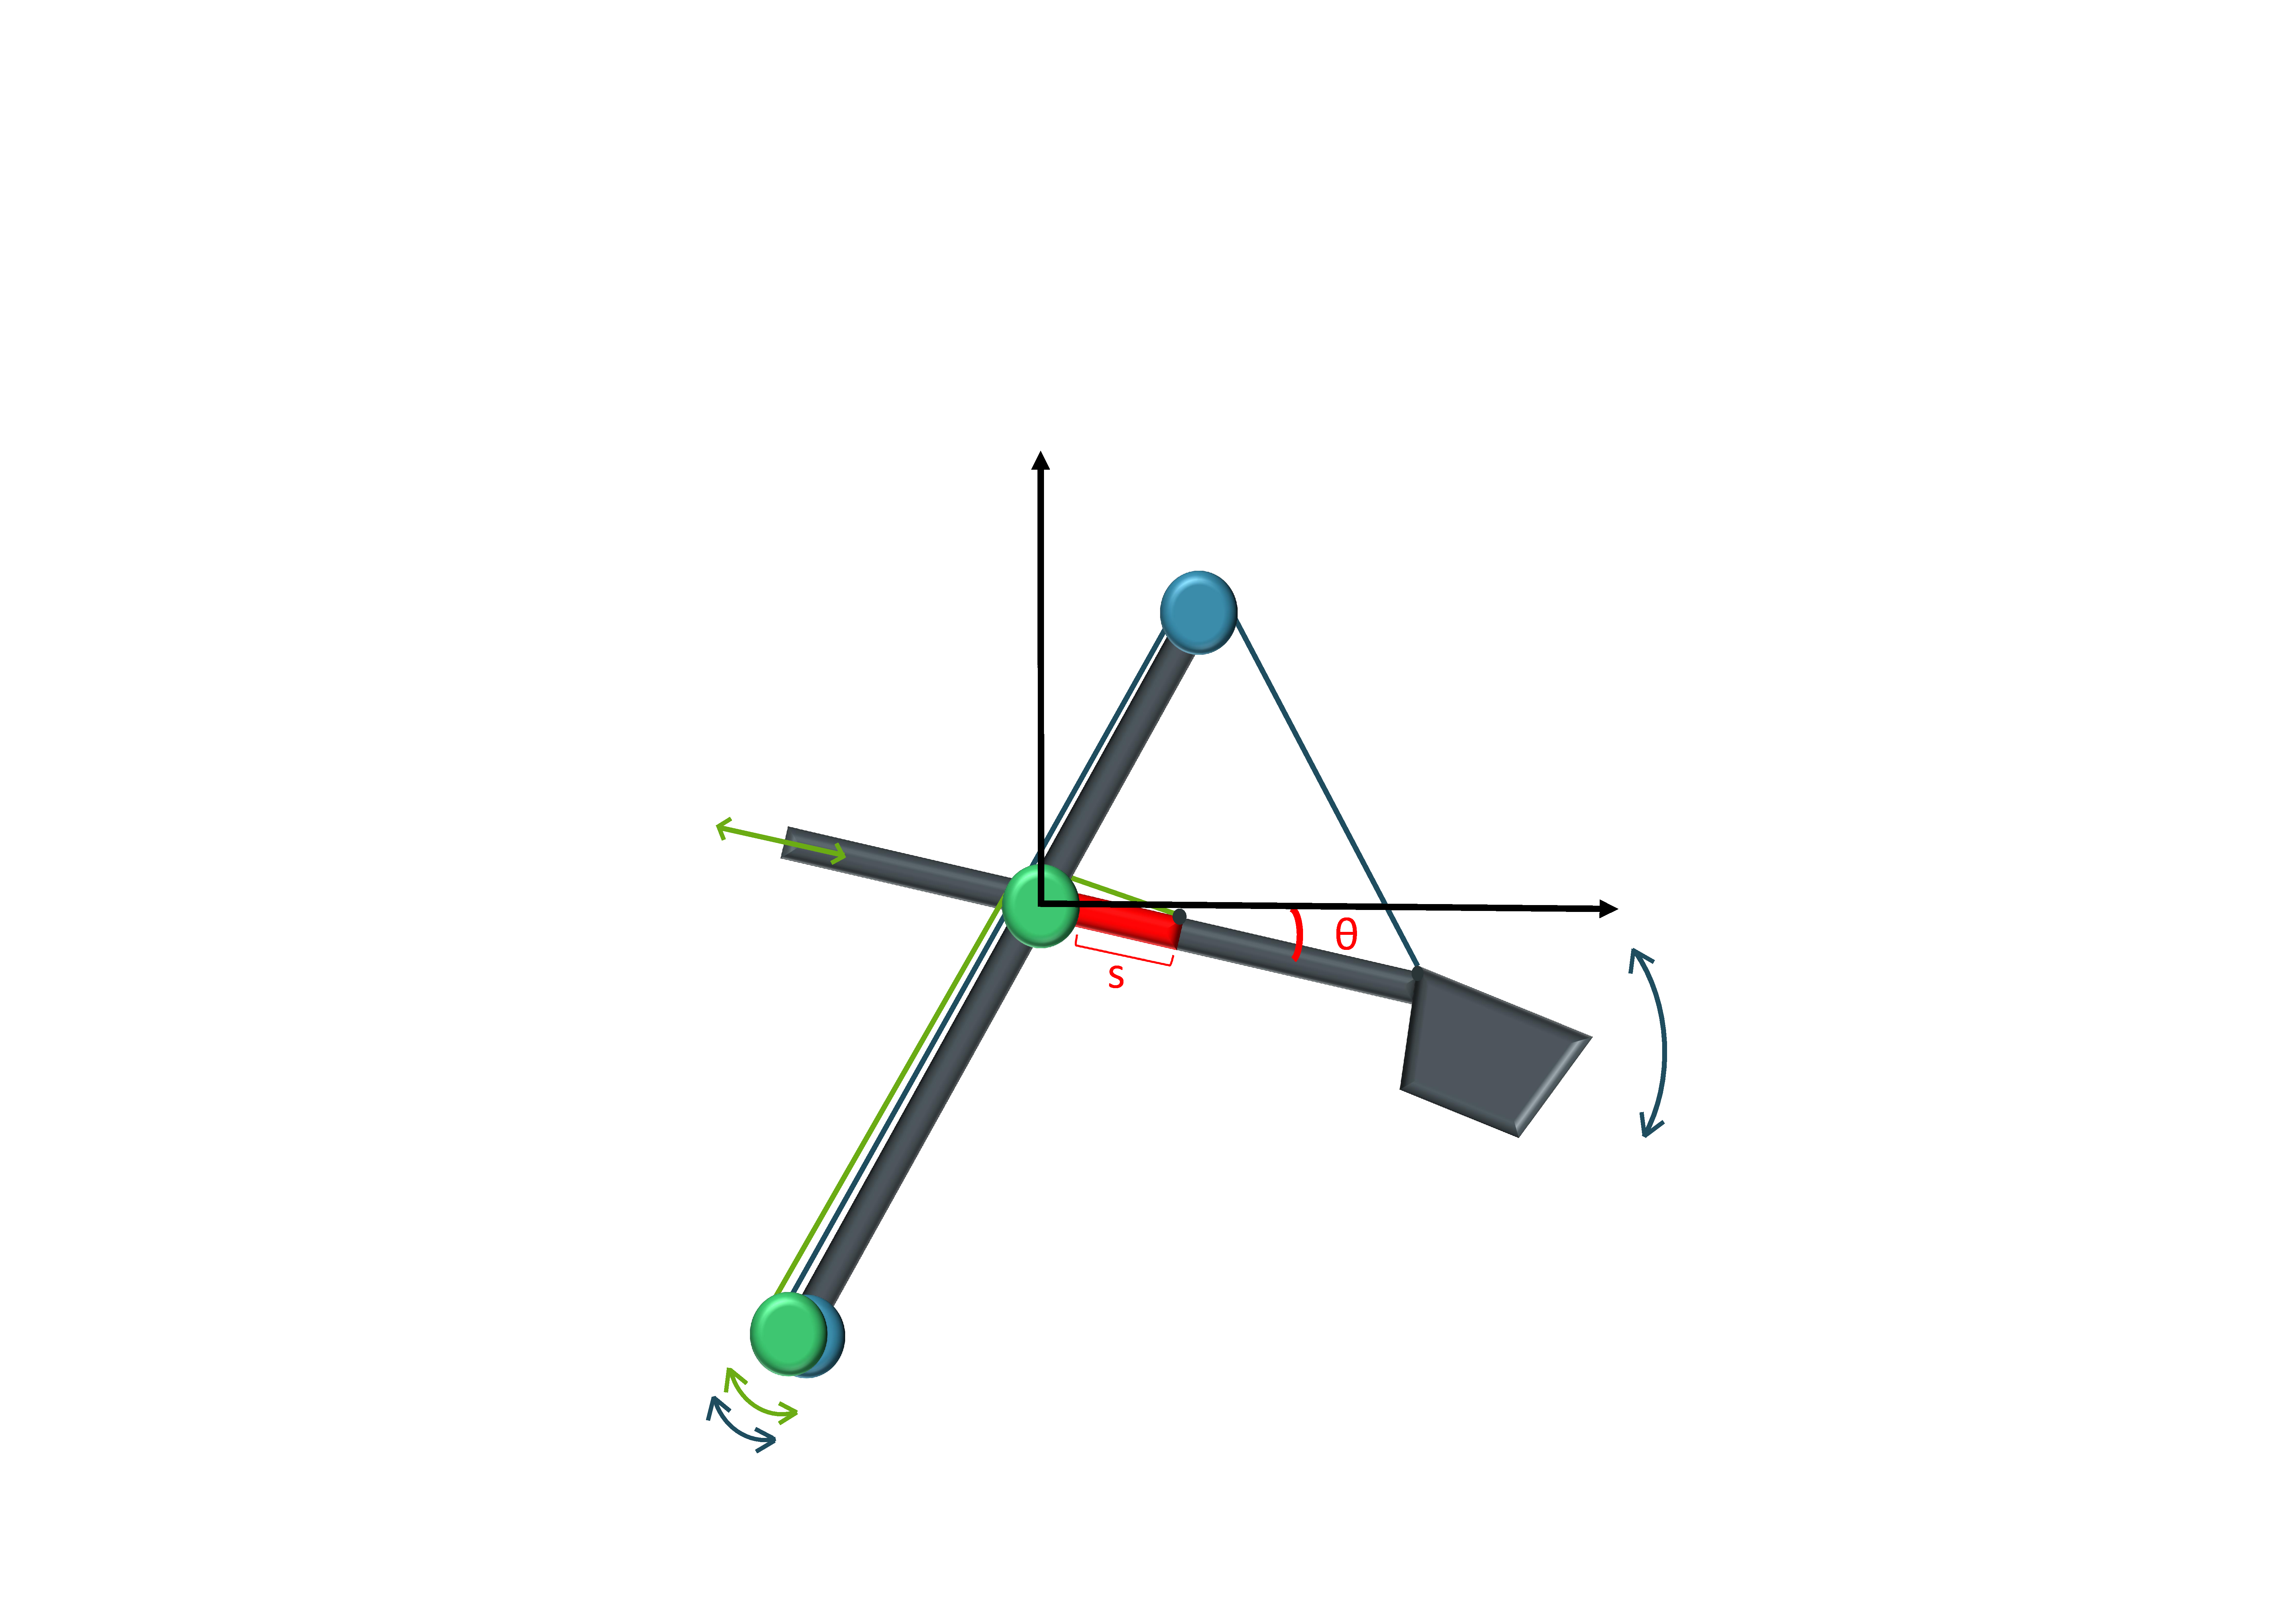
\includegraphics[trim=22cm 5cm 2cm 23cm, clip=true, width=\linewidth]{img/Excavator_dof2}
	
	\begin{columns}
		\column{.6\linewidth}
			\centering
			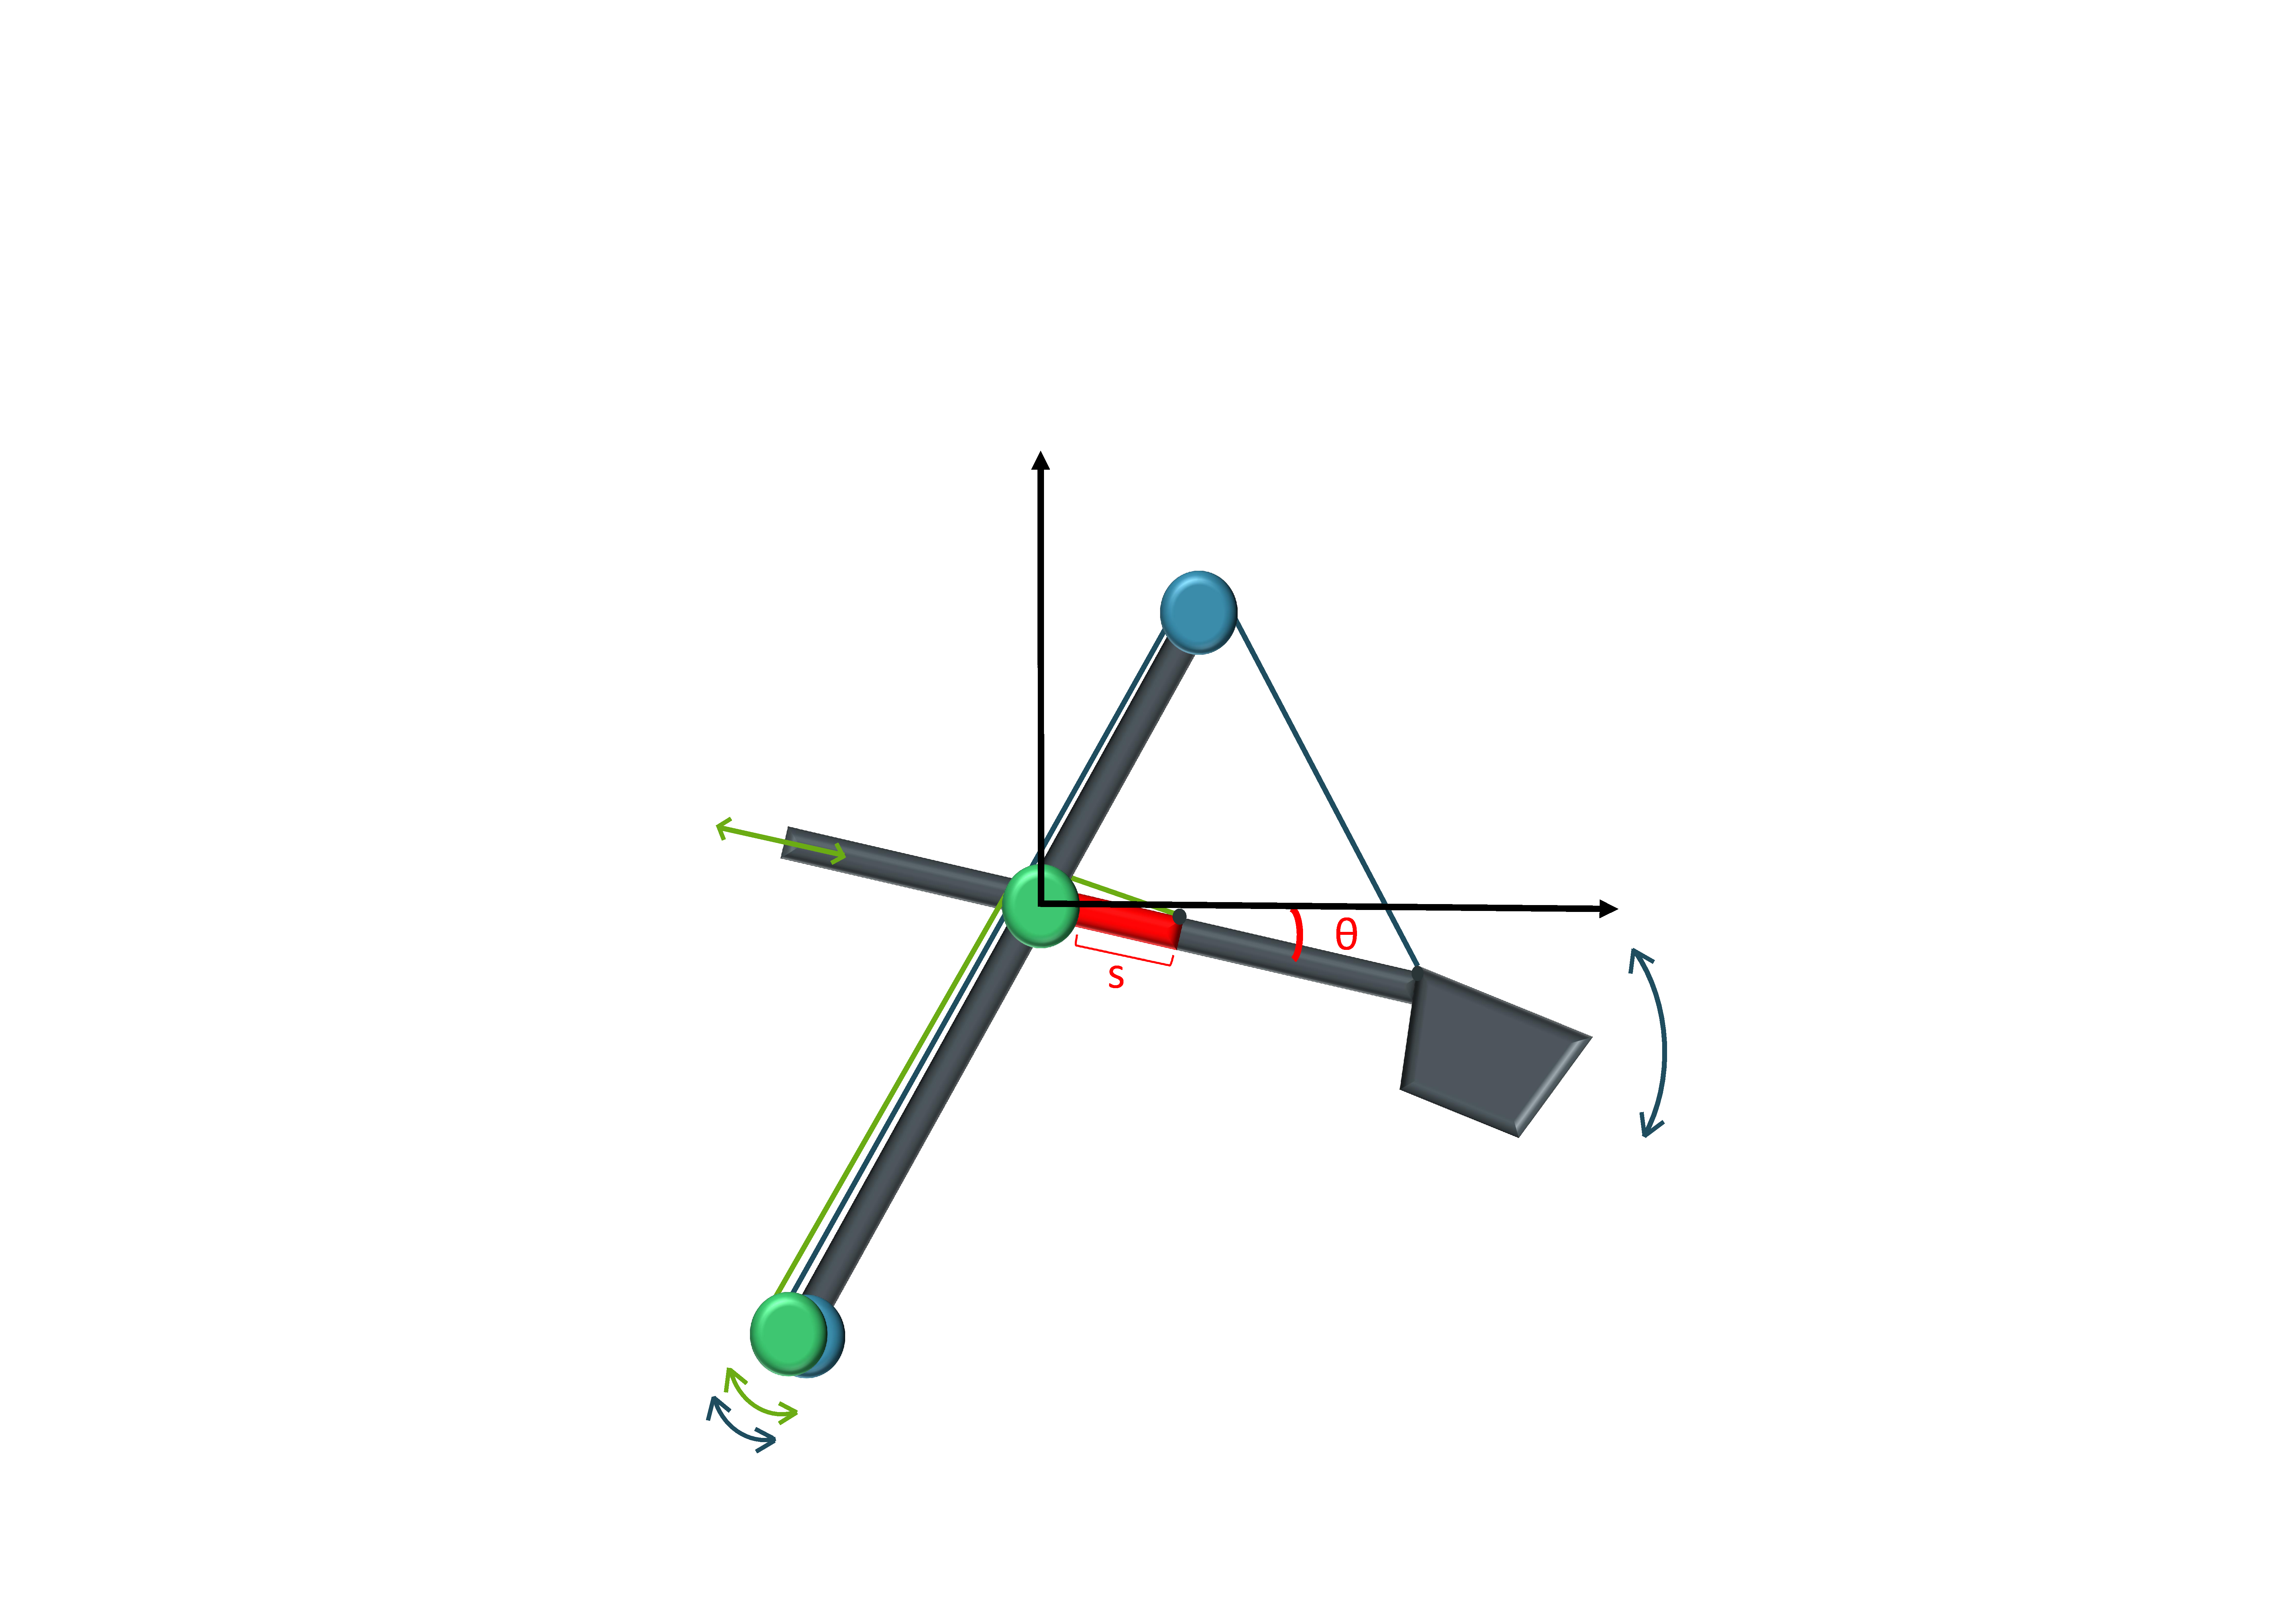
\includegraphics[trim=30cm 5cm 30cm 23cm, clip=true, width=\linewidth]{img/Excavator_dof2}
		\column{.4\linewidth}
			degrees of freedom
			\begin{itemize}
				\item{length $s$}
				\item{tilt angle $\theta$}
			\end{itemize}
	\end{columns}
	
	% s distance between attachment point and upper cable reel of green pulley
	
\end{frame}

\begin{frame}
	\frametitle{Physical Model of Excavator}
	
	%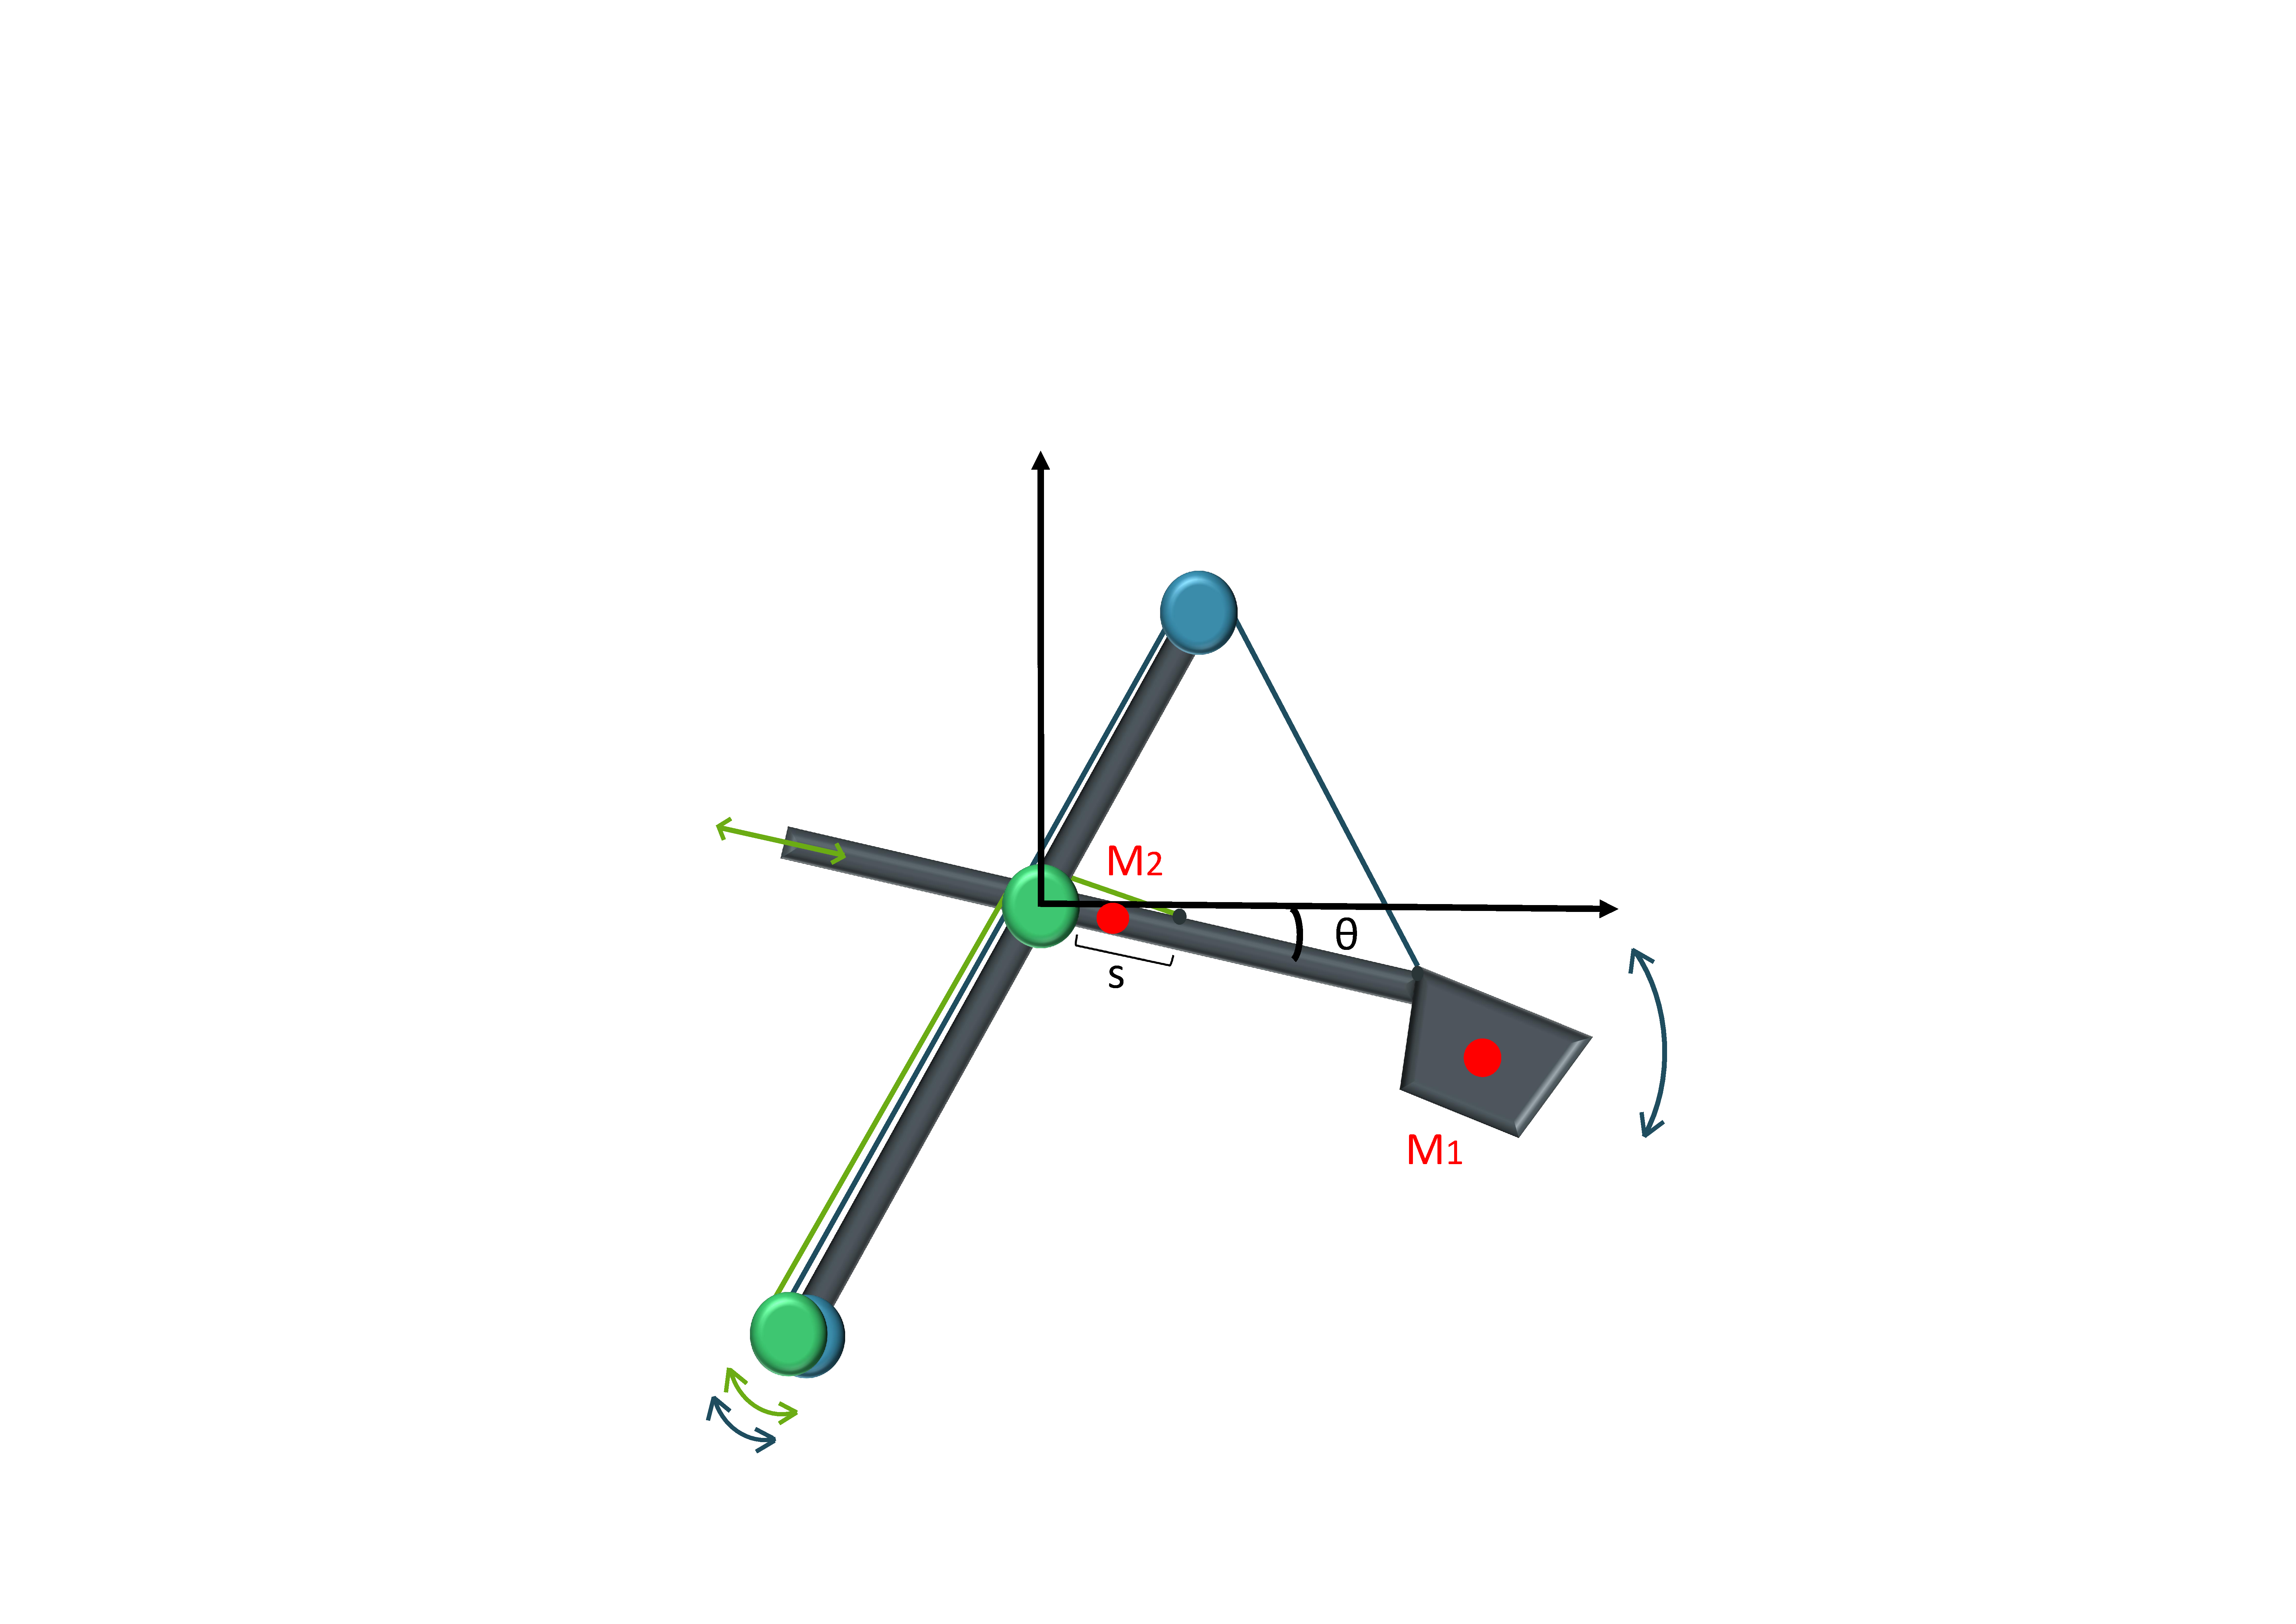
\includegraphics[trim=22cm 5cm 2cm 23cm, clip=true, width=\linewidth]{img/Excavator_mass2}
	
	\begin{columns}
		\column{.6\linewidth}
			\centering
			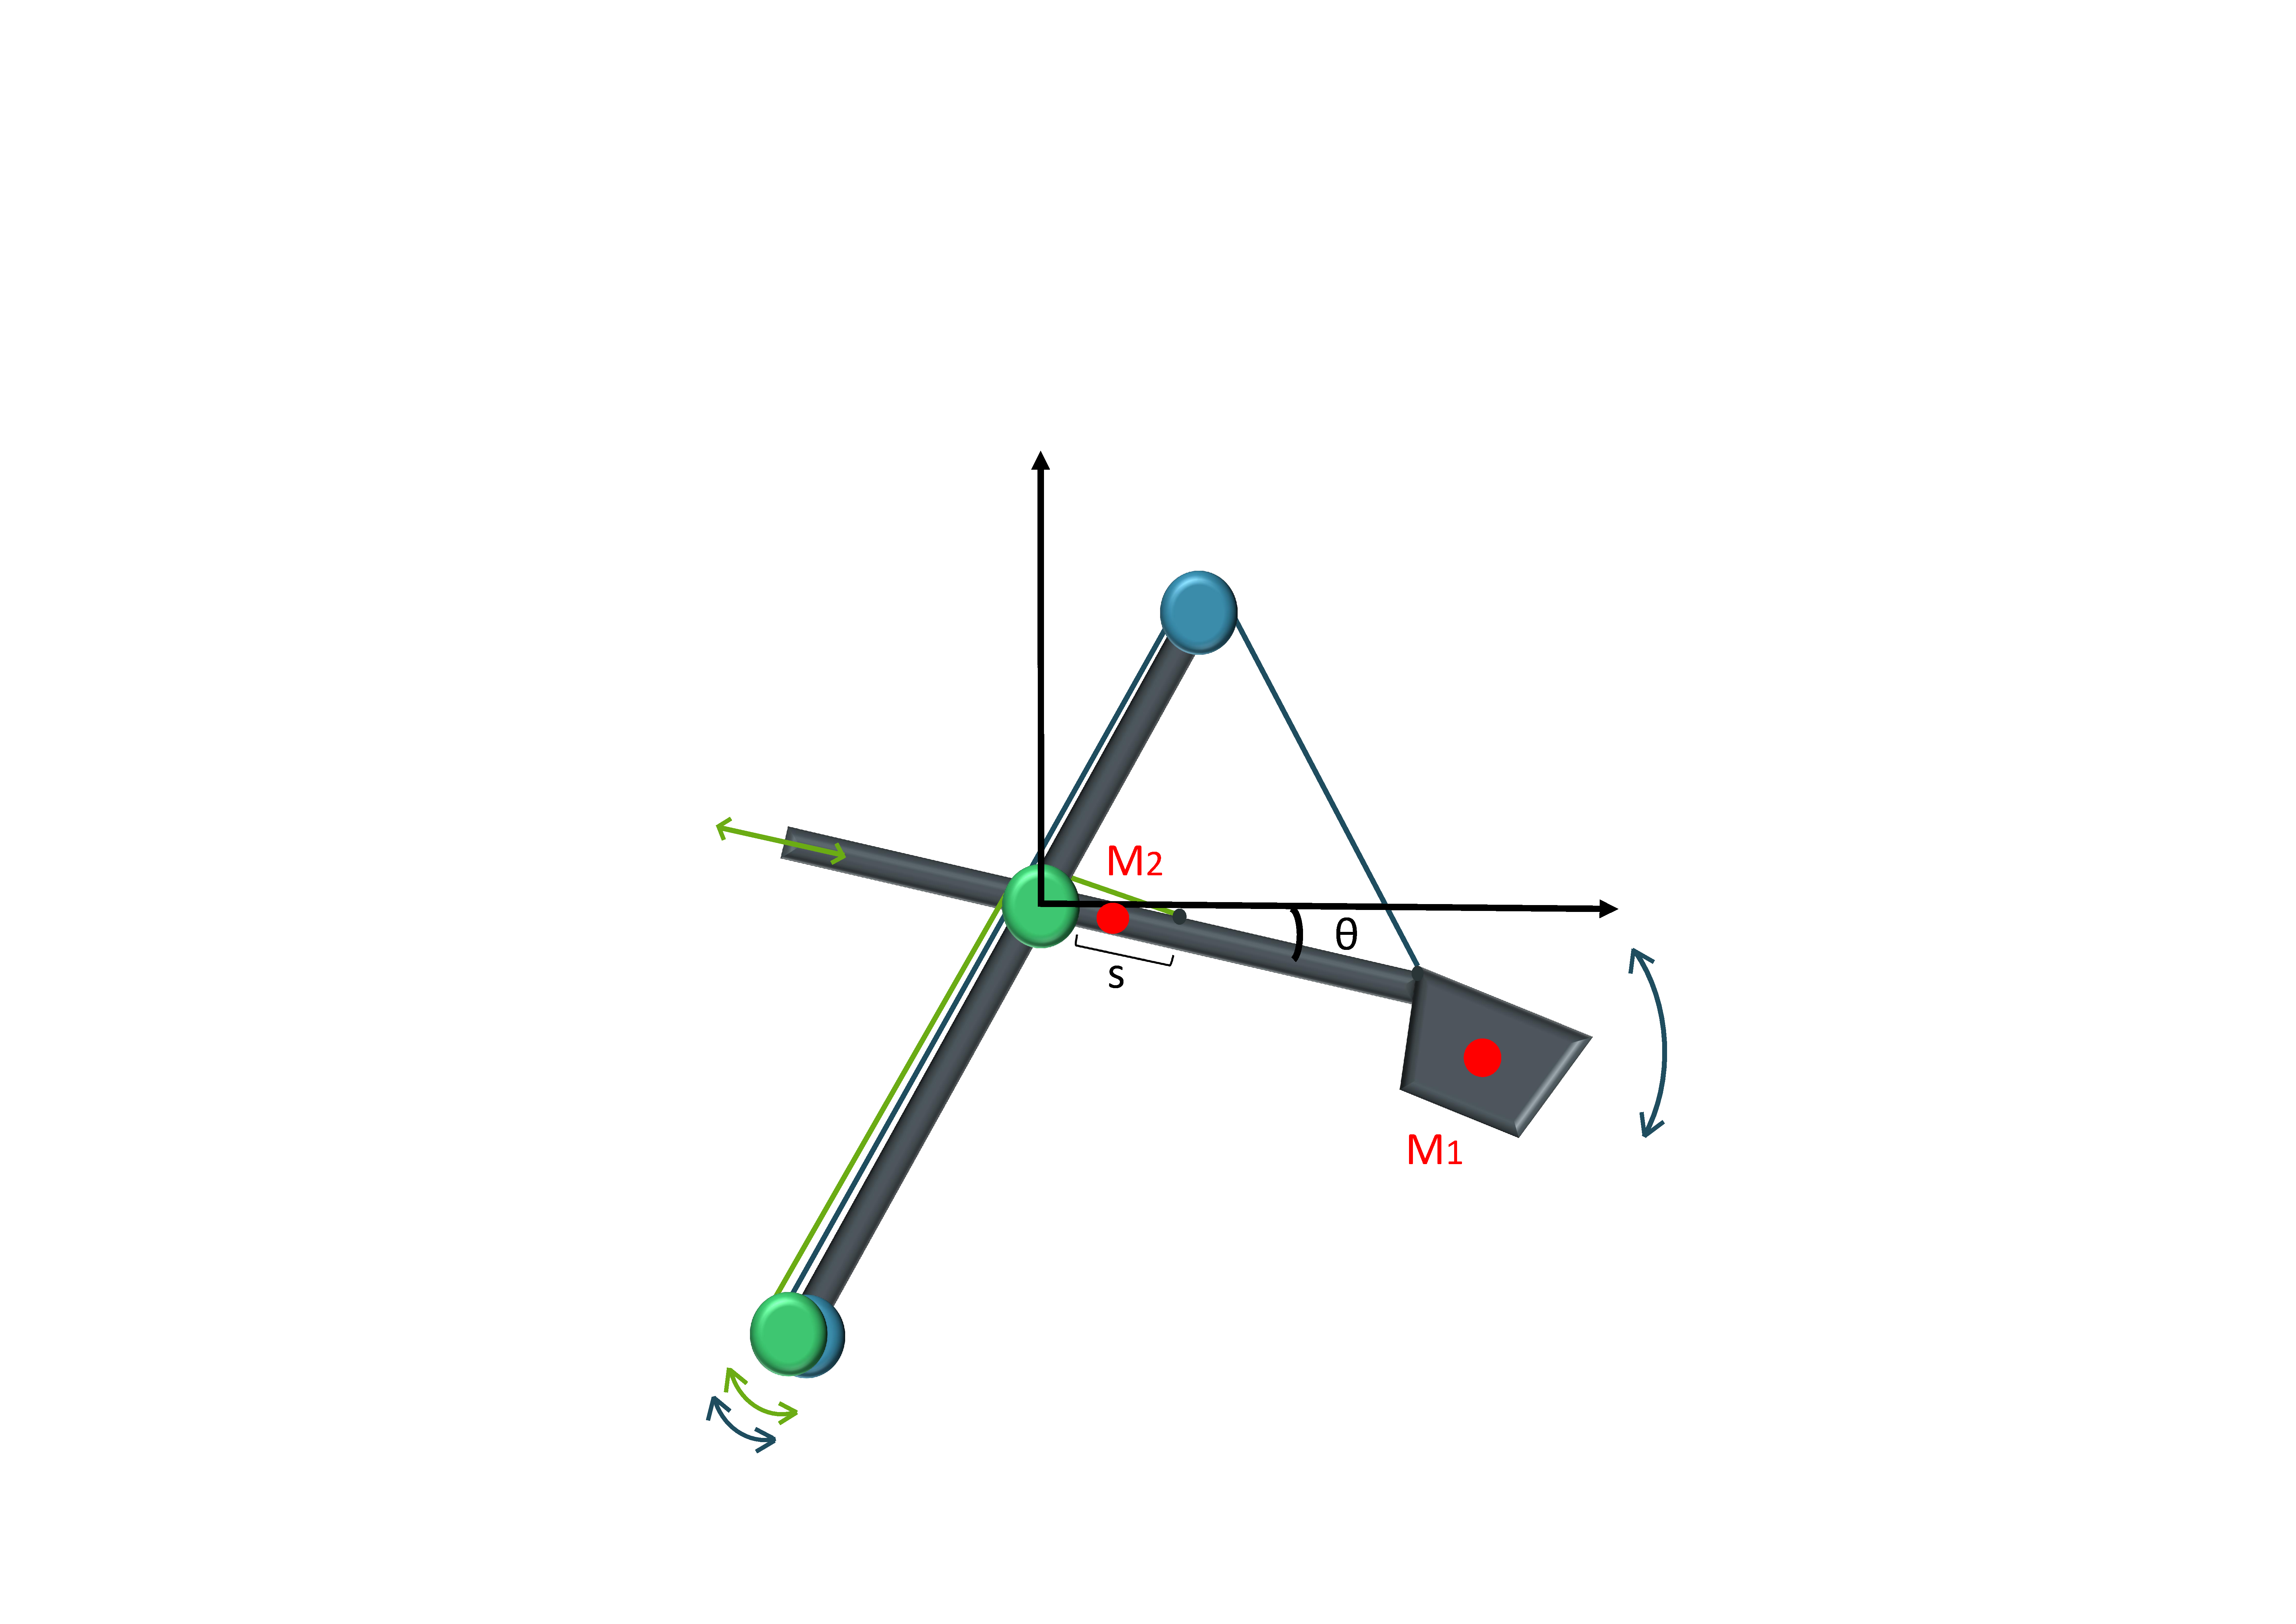
\includegraphics[trim=30cm 5cm 30cm 23cm, clip=true, width=\linewidth]{img/Excavator_mass2}
		\column{.4\linewidth}
			movable centers of gravity of
			\begin{itemize}
				\item{shovel $M_1$}
				\item{arm $M_2$}
			\end{itemize}
	\end{columns}
	
\end{frame}

\begin{frame}
	\frametitle{Physical Model of Excavator}
	
	%where are the point masses? only consider point masses which can be moved i.e. depend on configuration $\rightarrow$ derivative wrt degrees of freedom\\
	%shovel and center of mass of side arm\\
	%other arm is fixed and cant be moved
	
	Assumptions to the model:\\
	$ $ \\
	\begin{itemize}
		\item no mass for the ropes
		\item shovel as point mass % attached on the side arm
		\item no slack/friction between ropes and cable reels
		% ropes and cable reel move with same velocity
		% only bearing friction (friction within cable reels)
	\end{itemize}
	
\end{frame}

%\begin{frame}
	%\frametitle{Kinetic Energy T}
	%
	%Example: energies of $M_2$ 
	%\begin{align*}
		%&E_{\text{kin},M_2} = \frac{1}{2}\ M_2\ \| 
		%v_{O,M_2}(s,\theta,\dot{s},\dot{\theta}) \|^2 \\
		%&E_{\text{rot},M_2} = \frac{1}{2}\ I_{M_2}(s)\ \dot{\theta}^2 \\
	%\end{align*}
	%
	%all kinetic energies:
	%\begin{align*}
	%T\ =\ \ & E_{\text{kin},M_1} + E_{\text{kin},M_2} + E_{\text{rot},M_2}  \\
	%& + E_{\text{rot},B_1} + E_{\text{rot},B_2} + E_{\text{rot},P_1} + E_{\text{rot},P_2} \\
	%\end{align*}
%\end{frame}

%\begin{frame}
	%\frametitle{Potential V}
	%
	%Example: potential of $M_2$
	%\begin{align*}
		%& V_{M_2} = M_2\ g\ h(s,\theta) \\
	%\end{align*}
	%
	%all potentials:
	%\begin{align*}
		%& V = V_{M_1} + V_{M_2} \\
	%\end{align*}
%\end{frame}

%\begin{frame}
	%\frametitle{Involved Forces}
	%\begin{figure}[bth]
	  %\begin{center}
	    %%left, bottom, right, top
	    %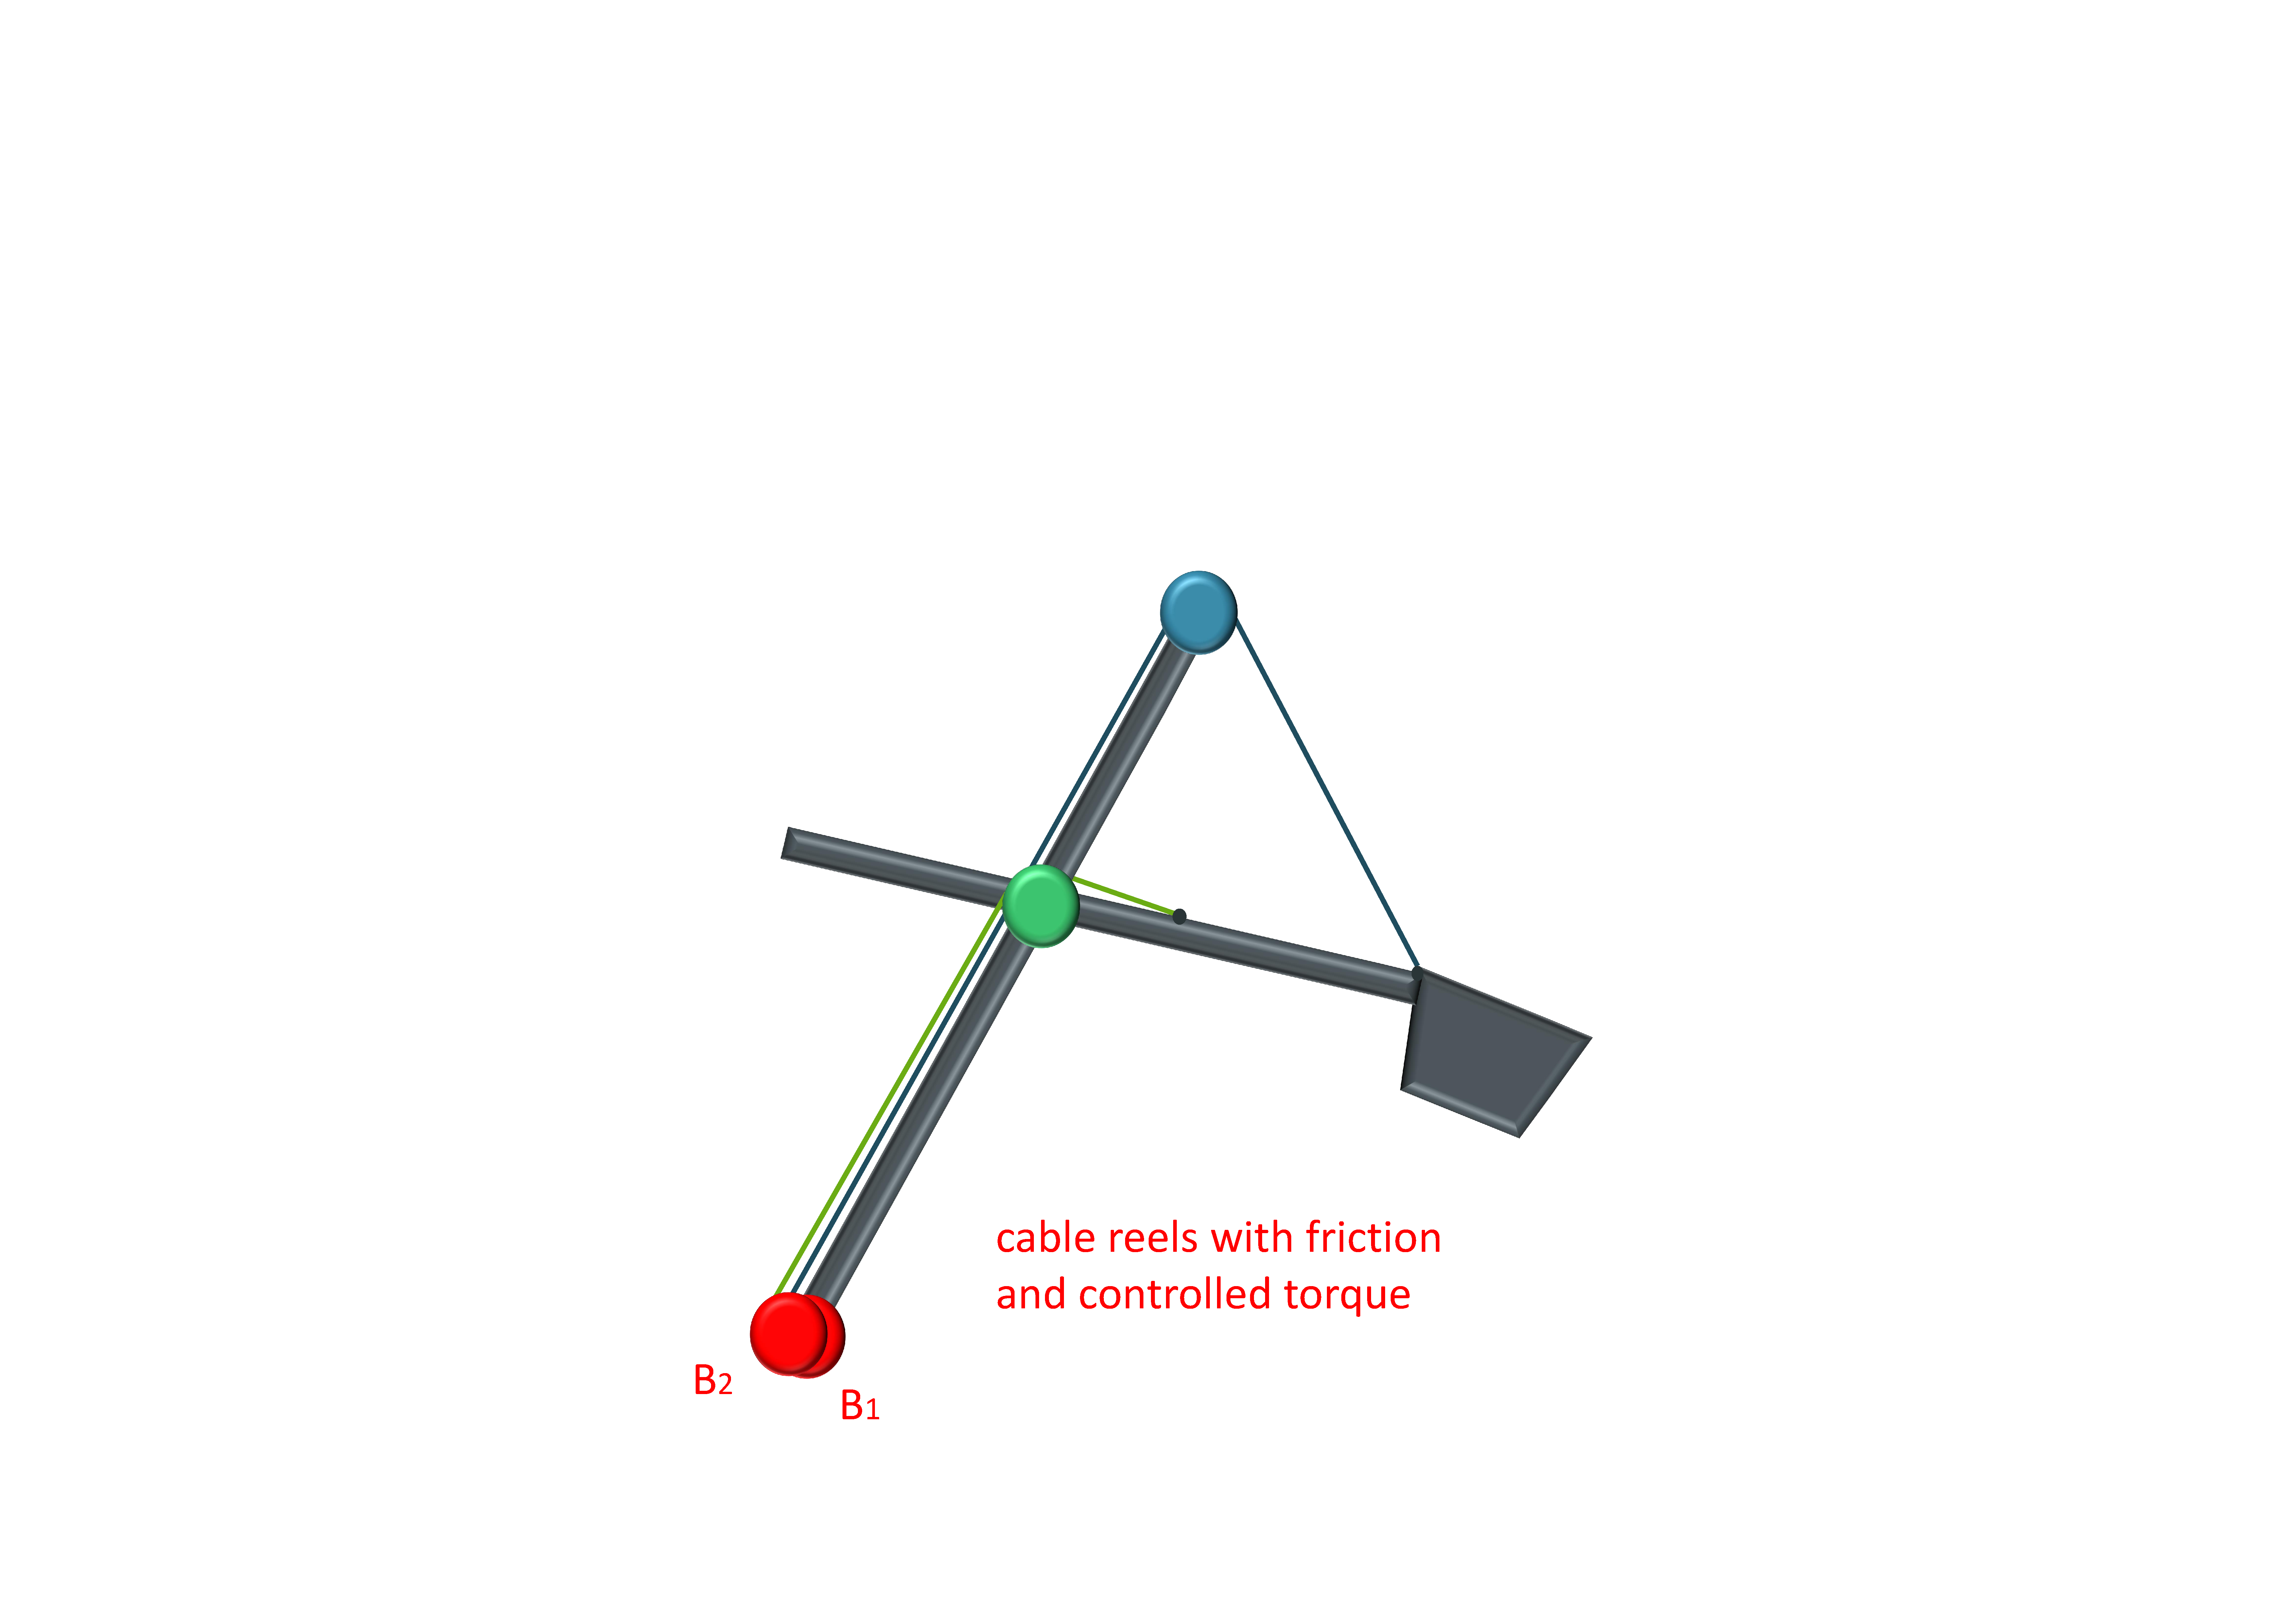
\includegraphics[trim=22cm 5cm 2cm 24cm, clip=true, 
	    %width=\linewidth]{img/Excavator_Only1}
	  %\end{center}
	%\end{figure}
%\end{frame}

\begin{frame}
	\frametitle{Kinetic Energy}
	\begin{columns}
		\column{.6\linewidth}
			\centering
			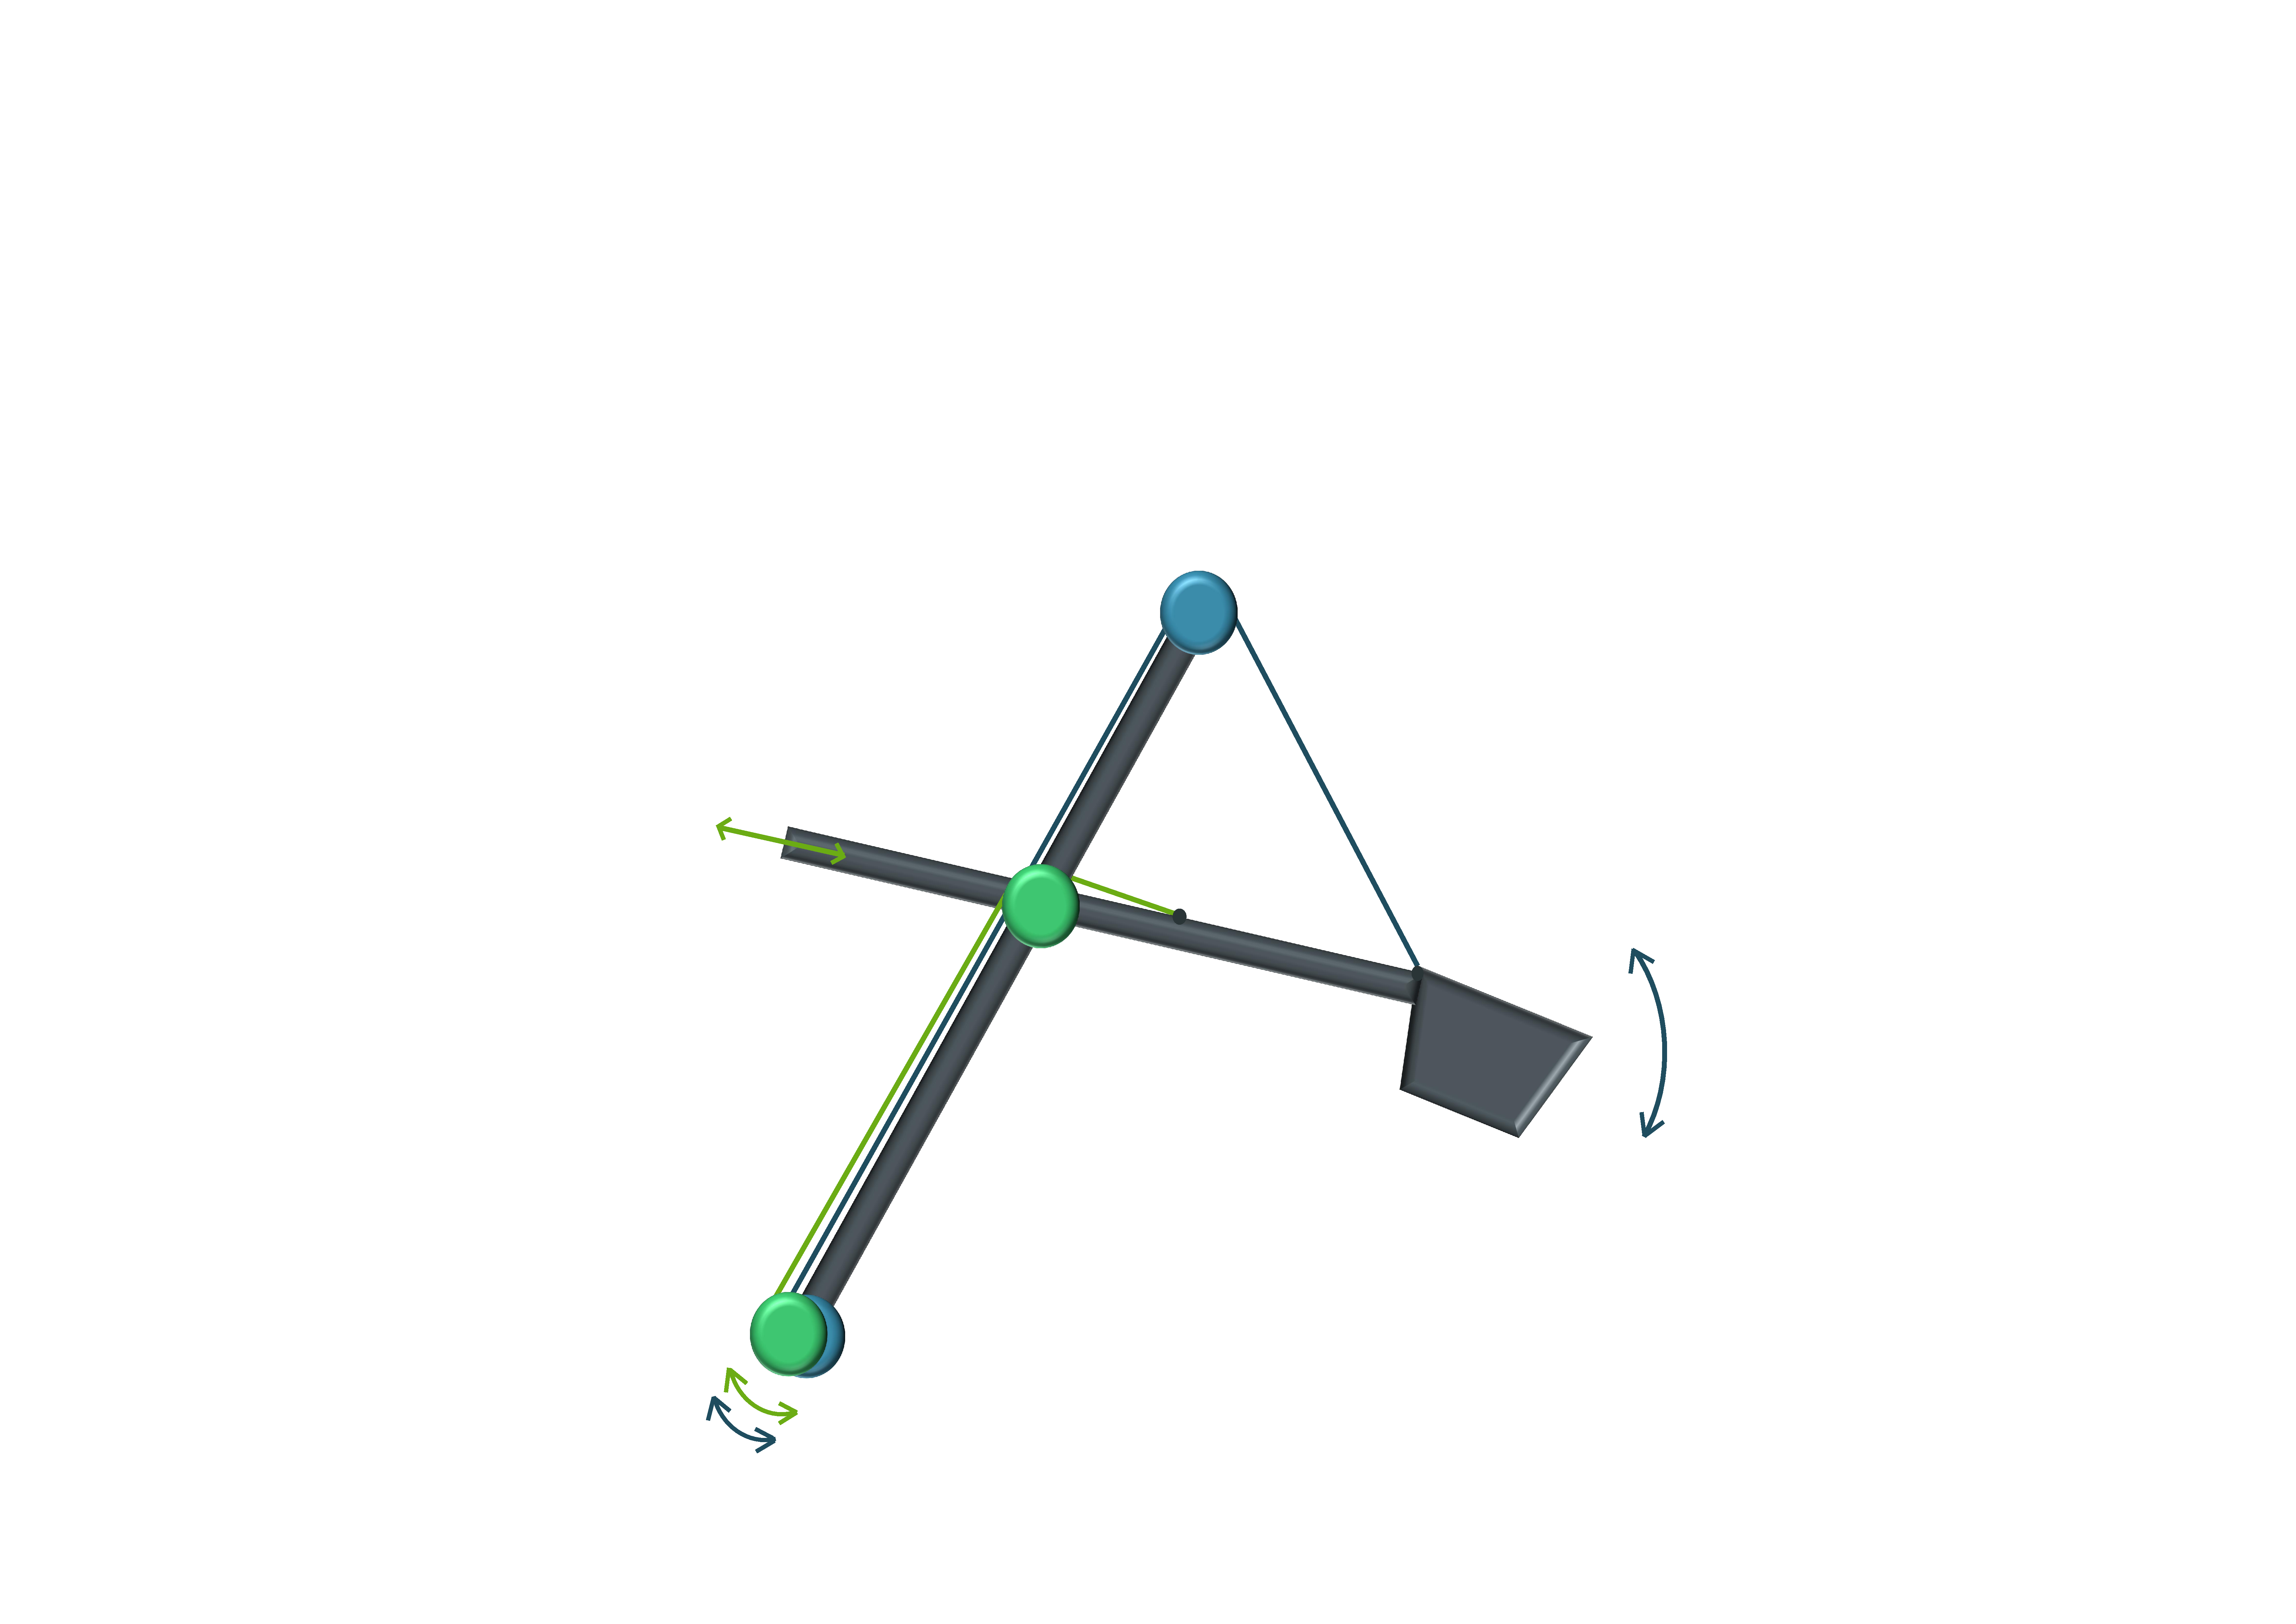
\includegraphics[trim=30cm 5cm 30cm 23cm, clip=true, width=\linewidth]{img/Excavator_Only}
		\column{.4\linewidth}
			\begin{itemize}
				\item{movement of mass}
				\item{rotation of cable reel}
			\end{itemize}
	\end{columns}
\end{frame}

%\begin{frame}
	%\frametitle{Involved Forces}
	%\begin{figure}[bth]
	  %\begin{center}
	    %%left, bottom, right, top
	    %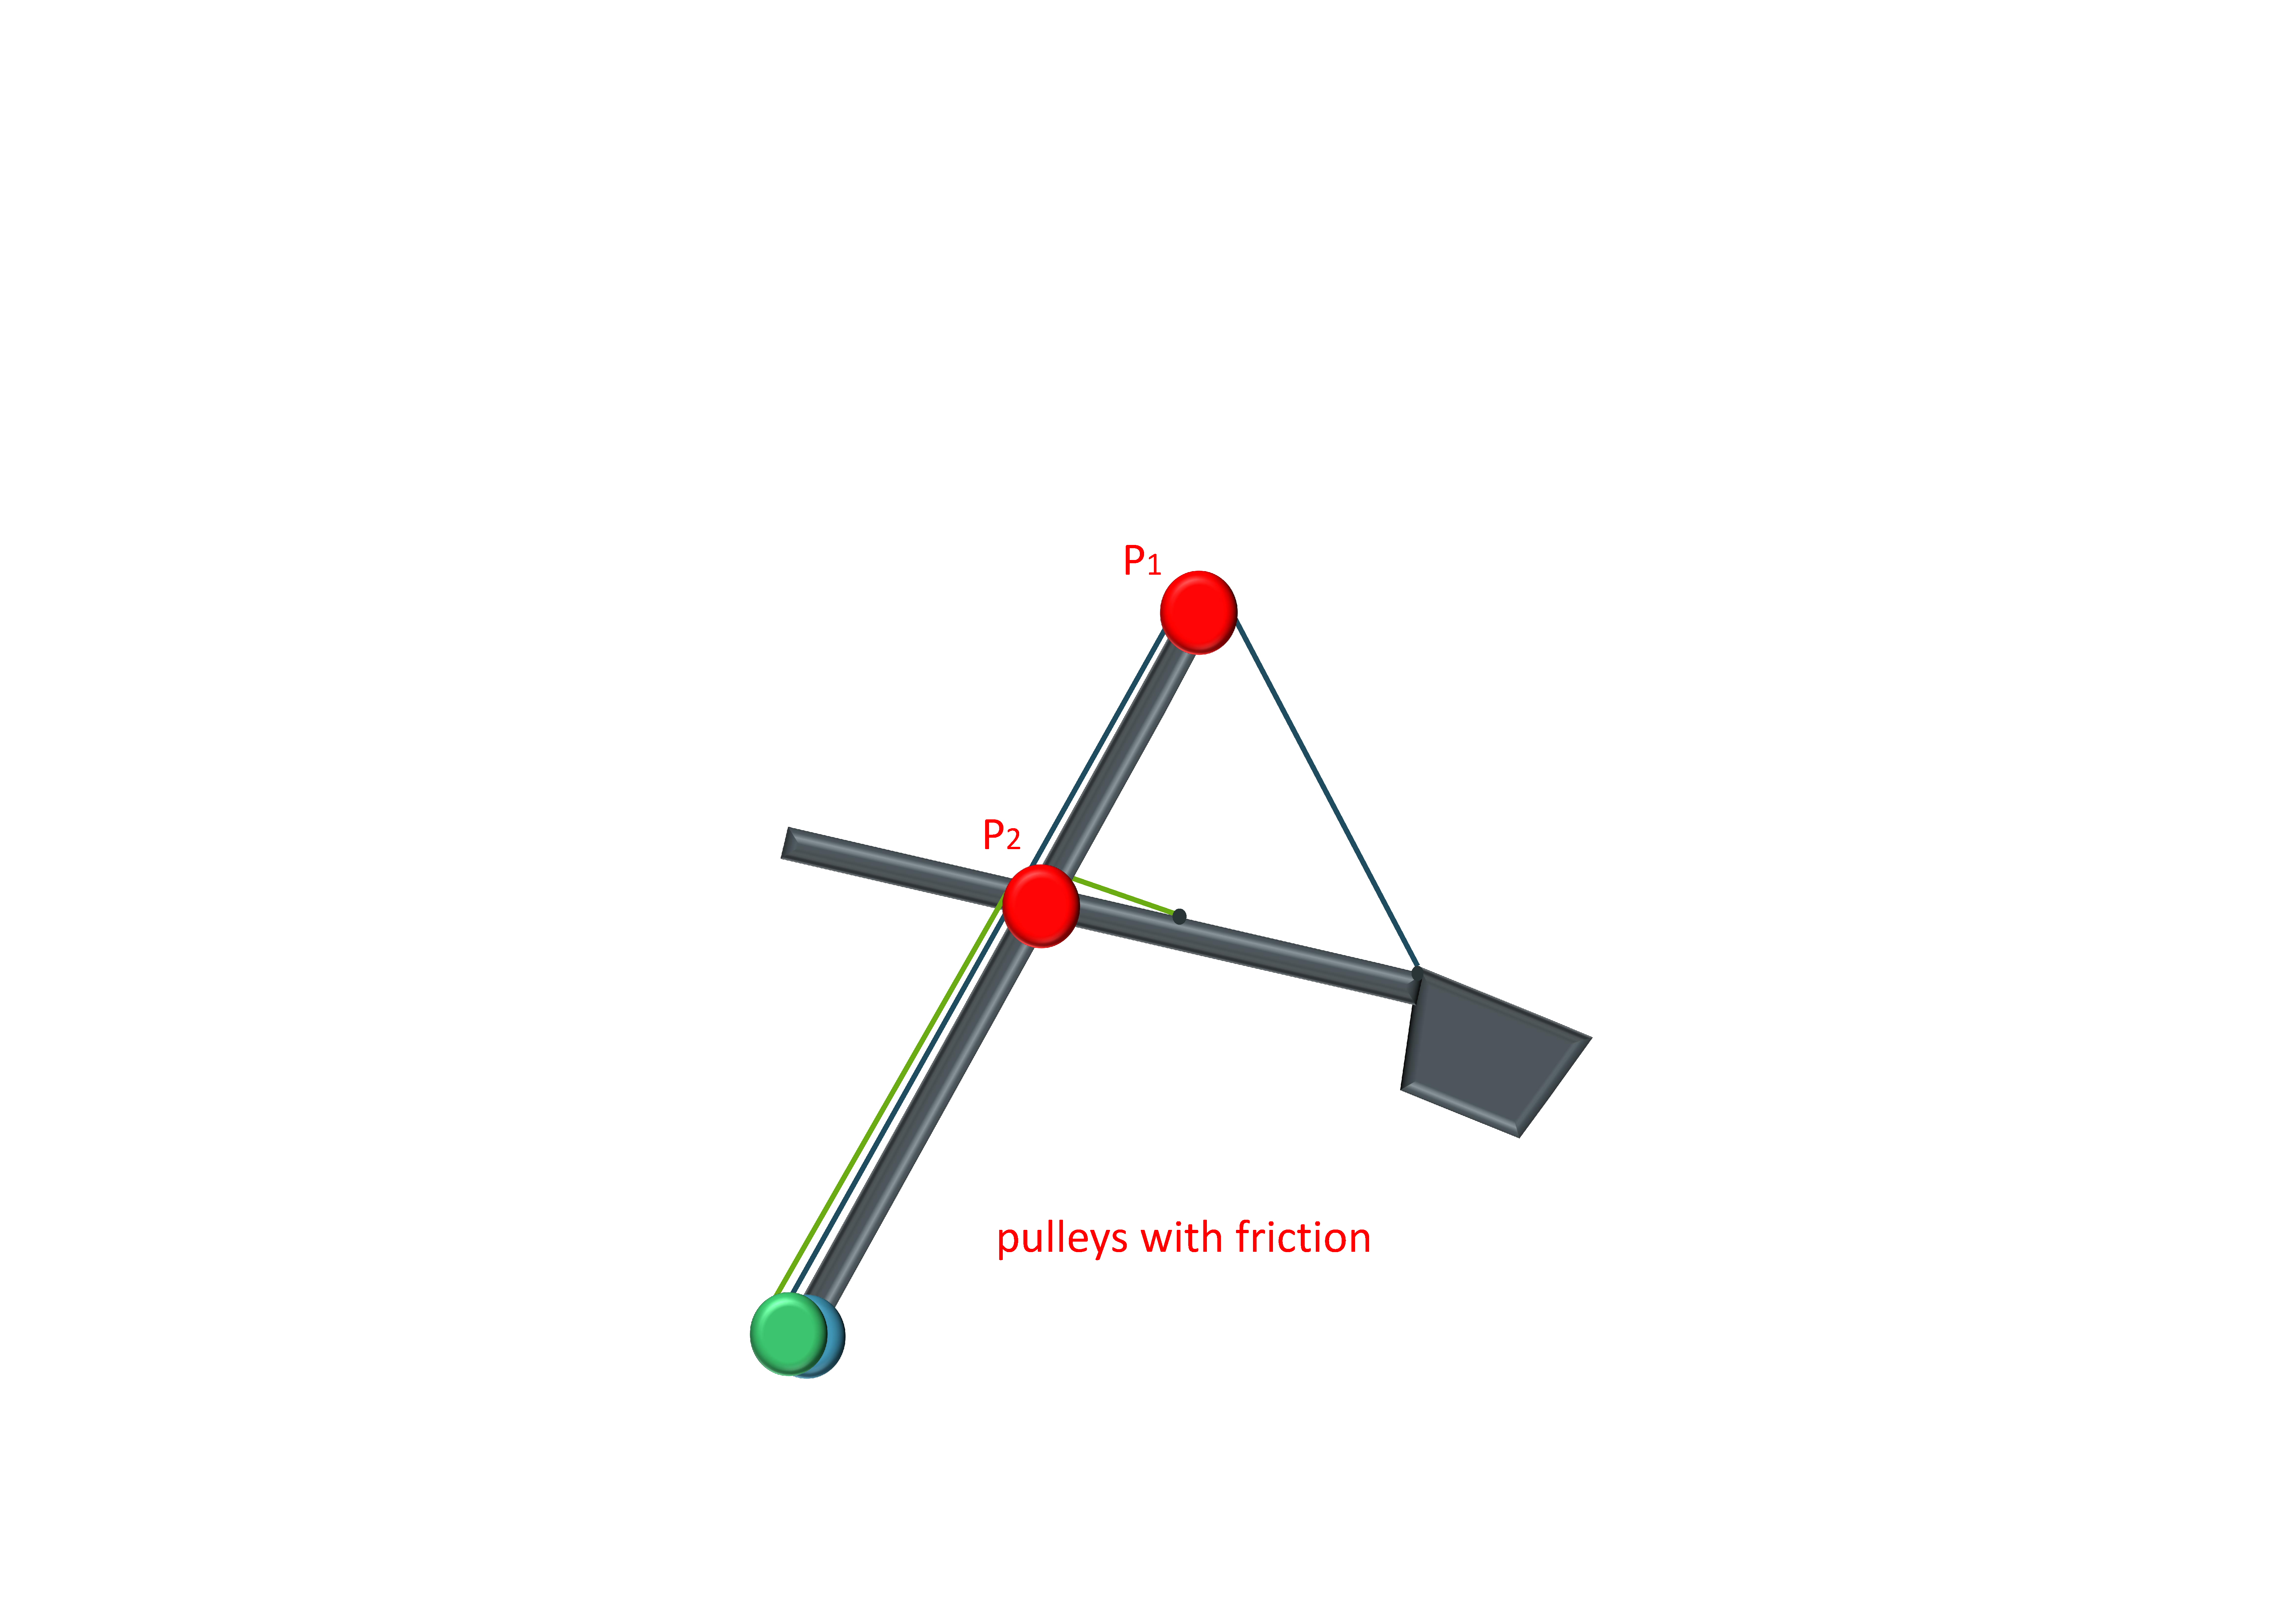
\includegraphics[trim=22cm 5cm 2cm 24cm, clip=true, 
	    %width=\linewidth]{img/Excavator_Only2}
	  %\end{center}
	%\end{figure}
%\end{frame}

\begin{frame}
	\frametitle{Potential Energy}
	\begin{columns}
		\column{.6\linewidth}
			\centering
			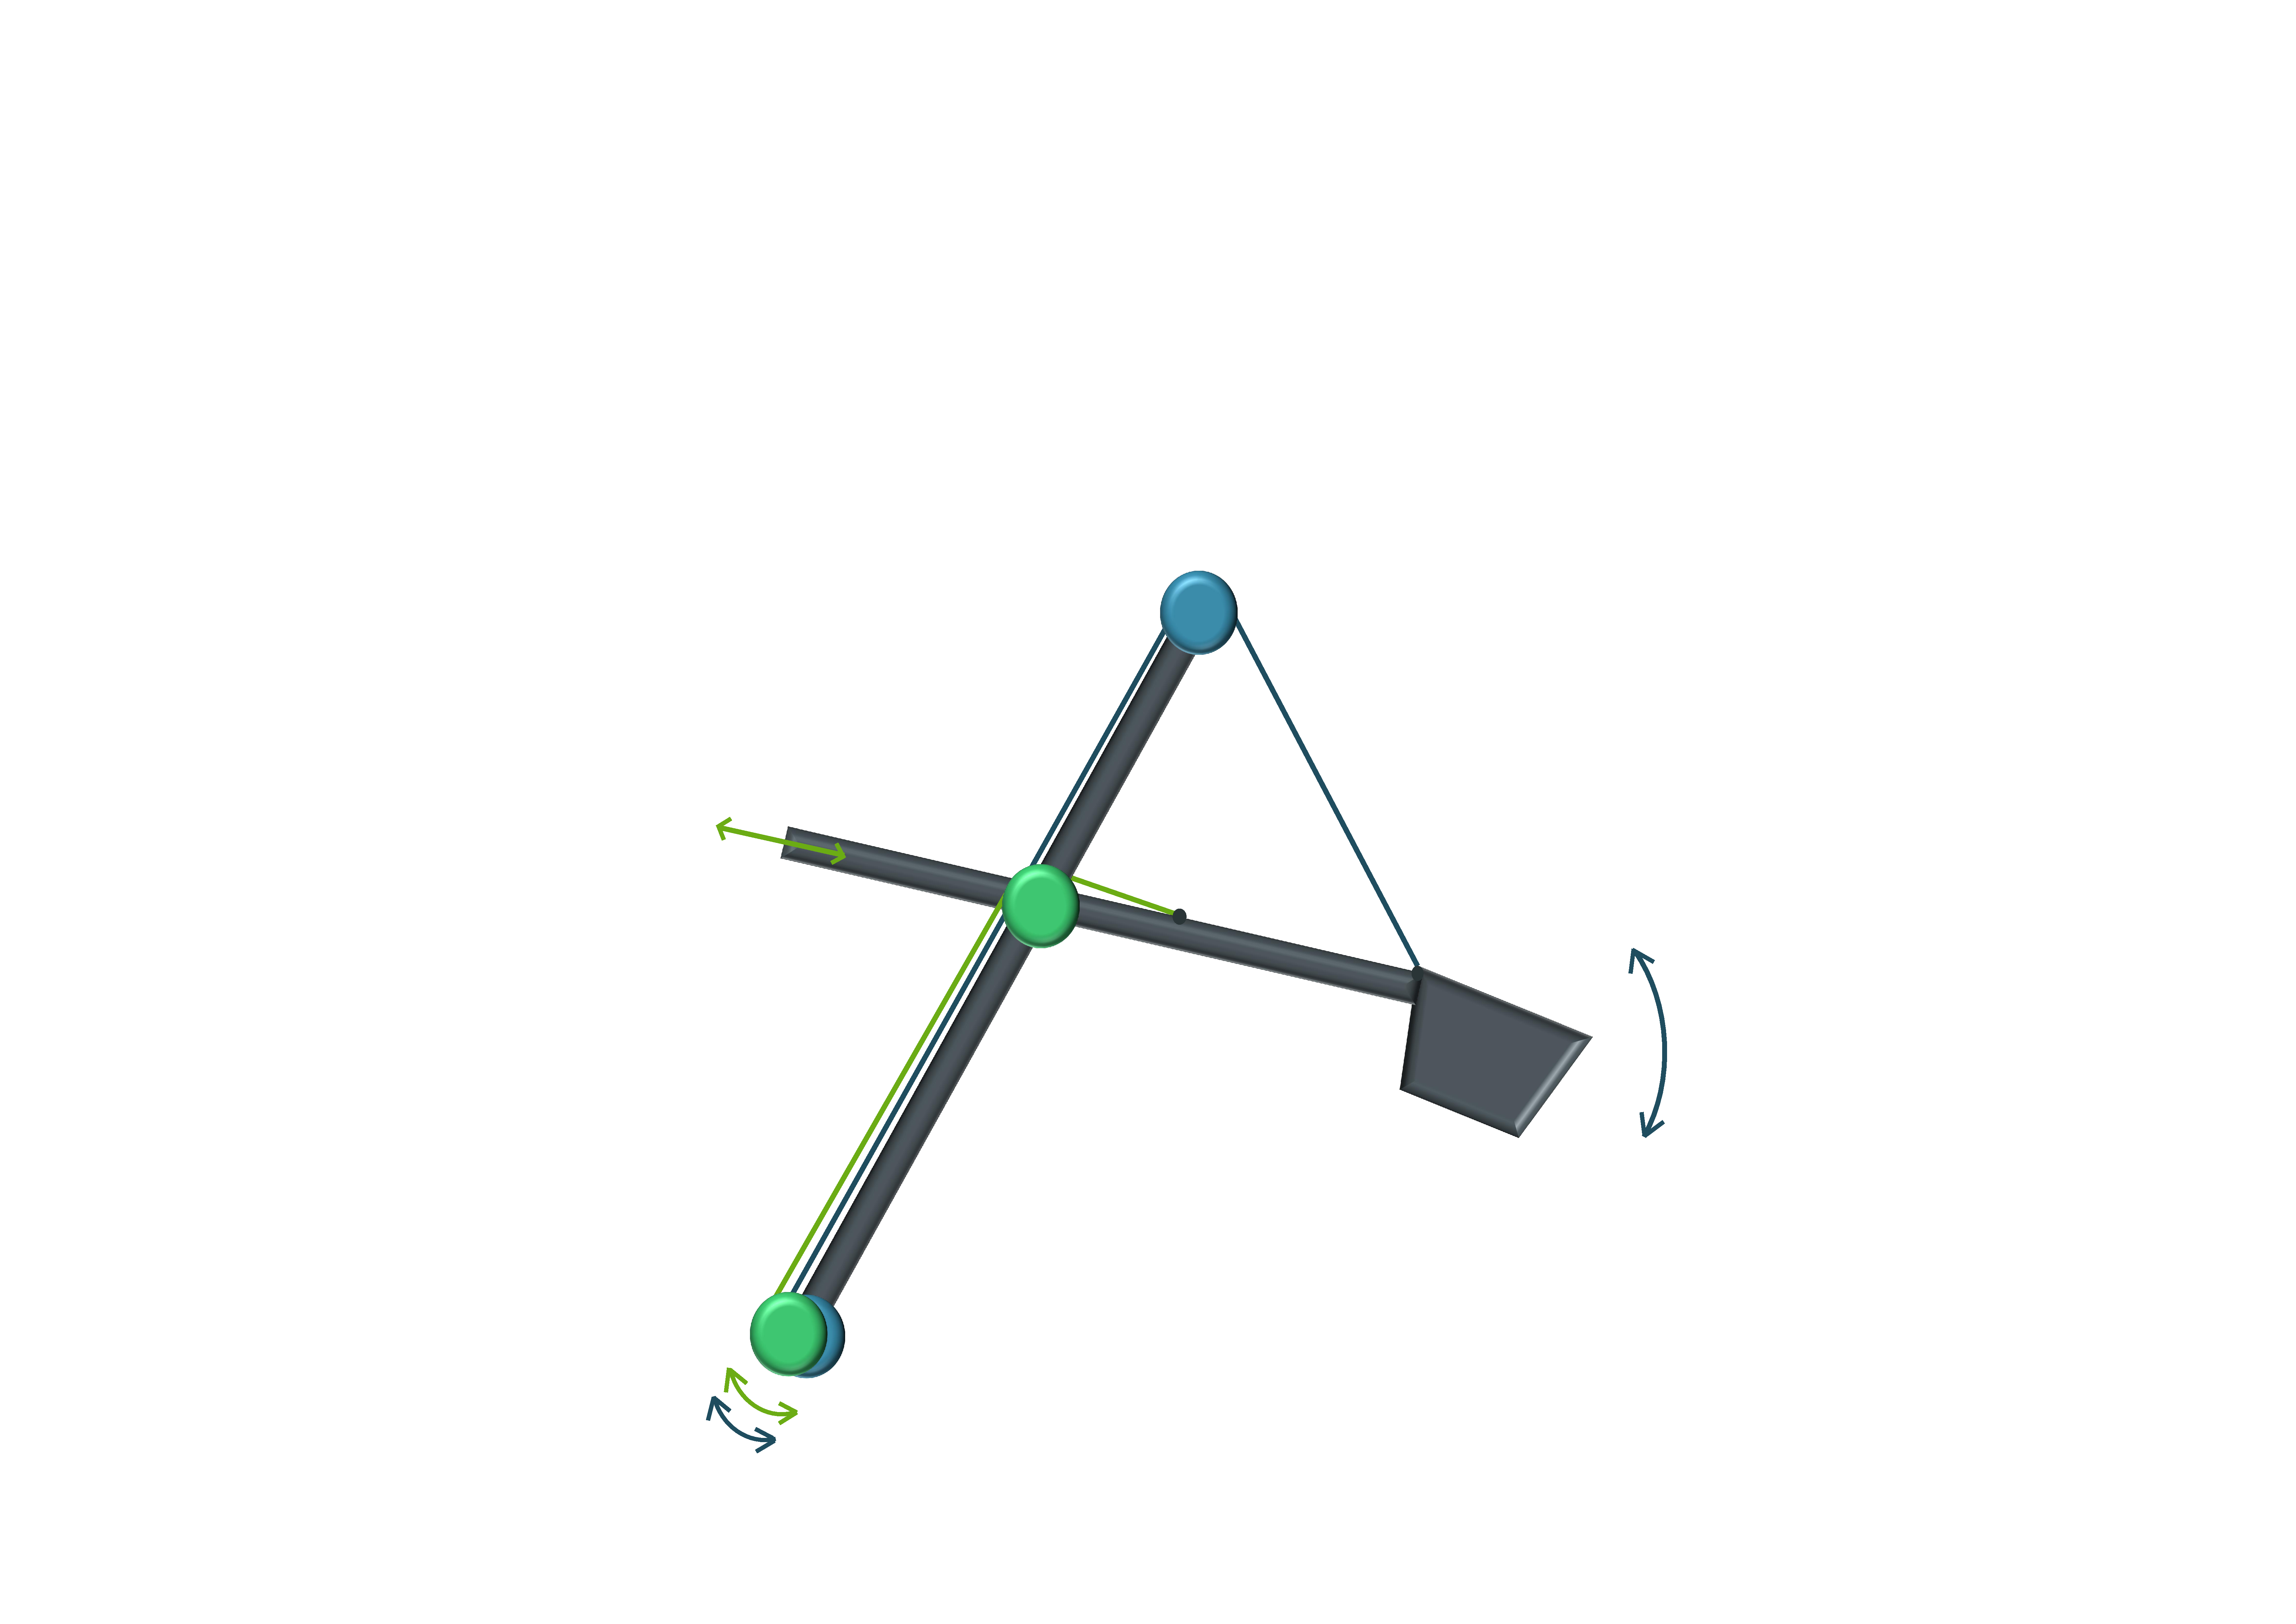
\includegraphics[trim=30cm 5cm 30cm 23cm, clip=true, width=\linewidth]{img/Excavator_Only}
		\column{.4\linewidth}
			gravitational potential energy
	\end{columns}
\end{frame}

%\begin{frame}
	%\frametitle{Involved Forces}
	%\begin{figure}[bth]
	  %\begin{center}
	    %%left, bottom, right, top
	    %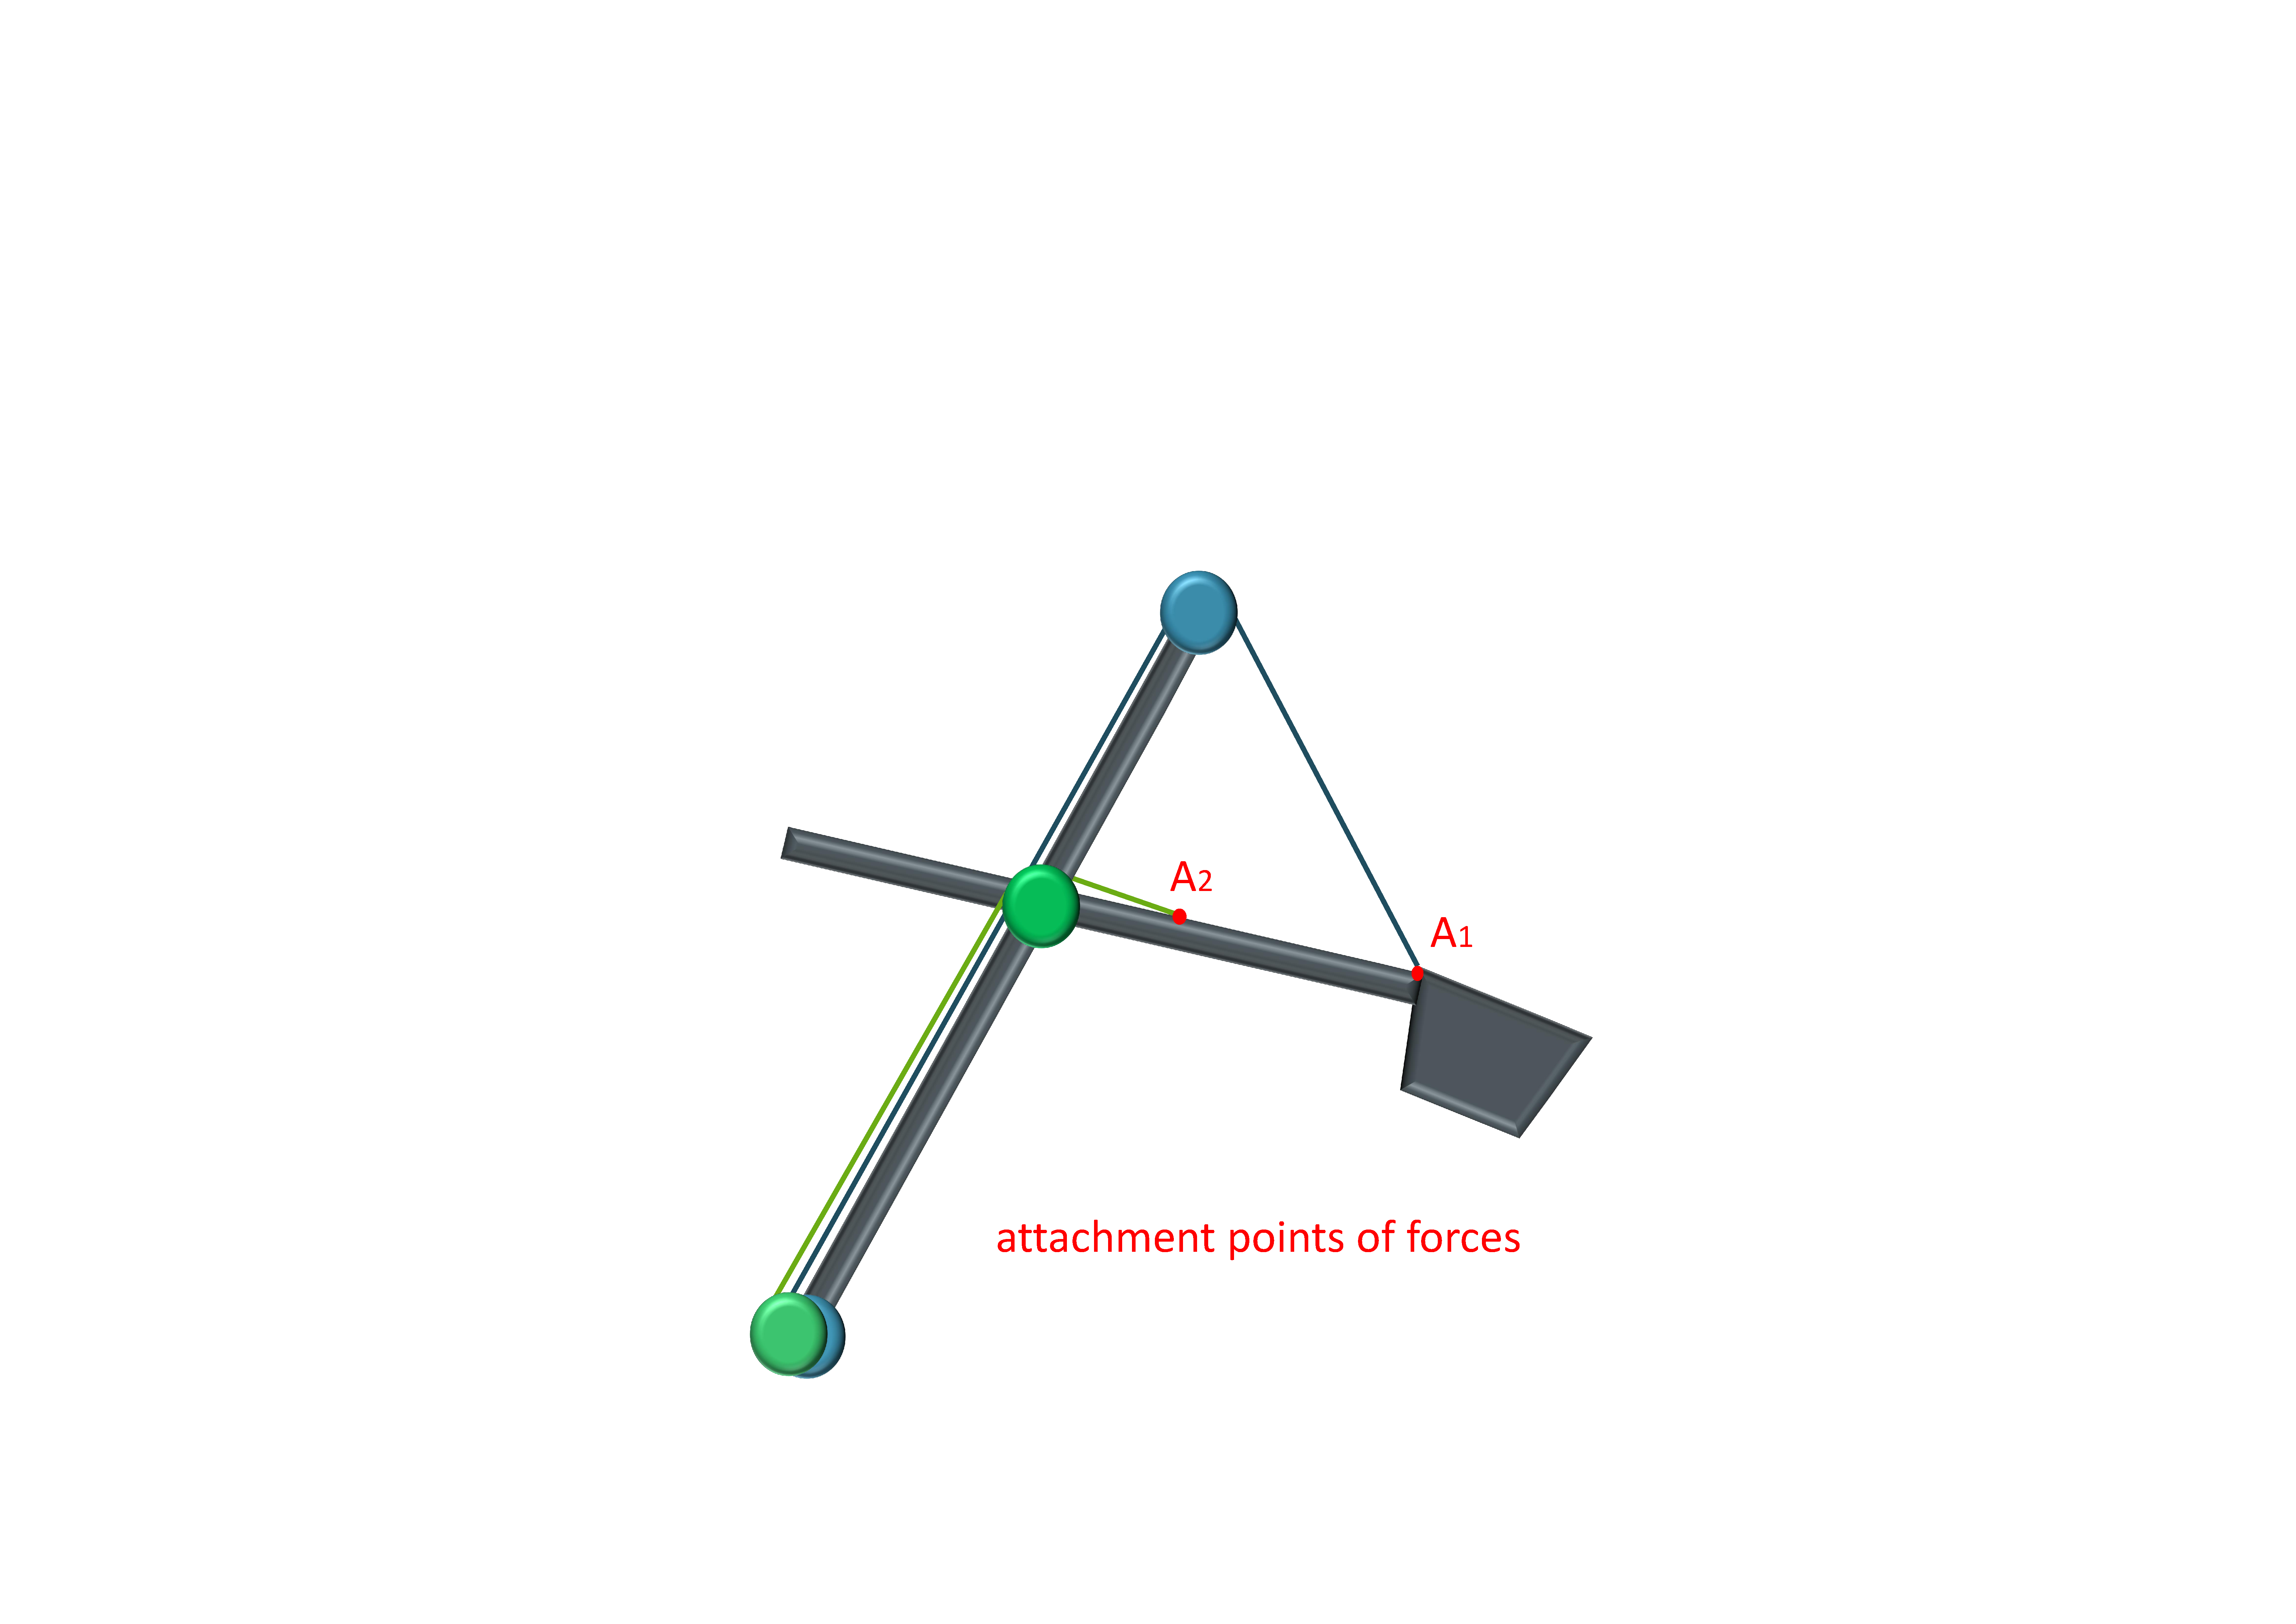
\includegraphics[trim=22cm 5cm 2cm 24cm, clip=true, 
	    %width=\linewidth]{img/Excavator_Only3}
	  %\end{center}
	%\end{figure}
%\end{frame}

\begin{frame}
	\frametitle{Generalized Forces}
	\begin{columns}
		\column{.6\linewidth}
			\centering
			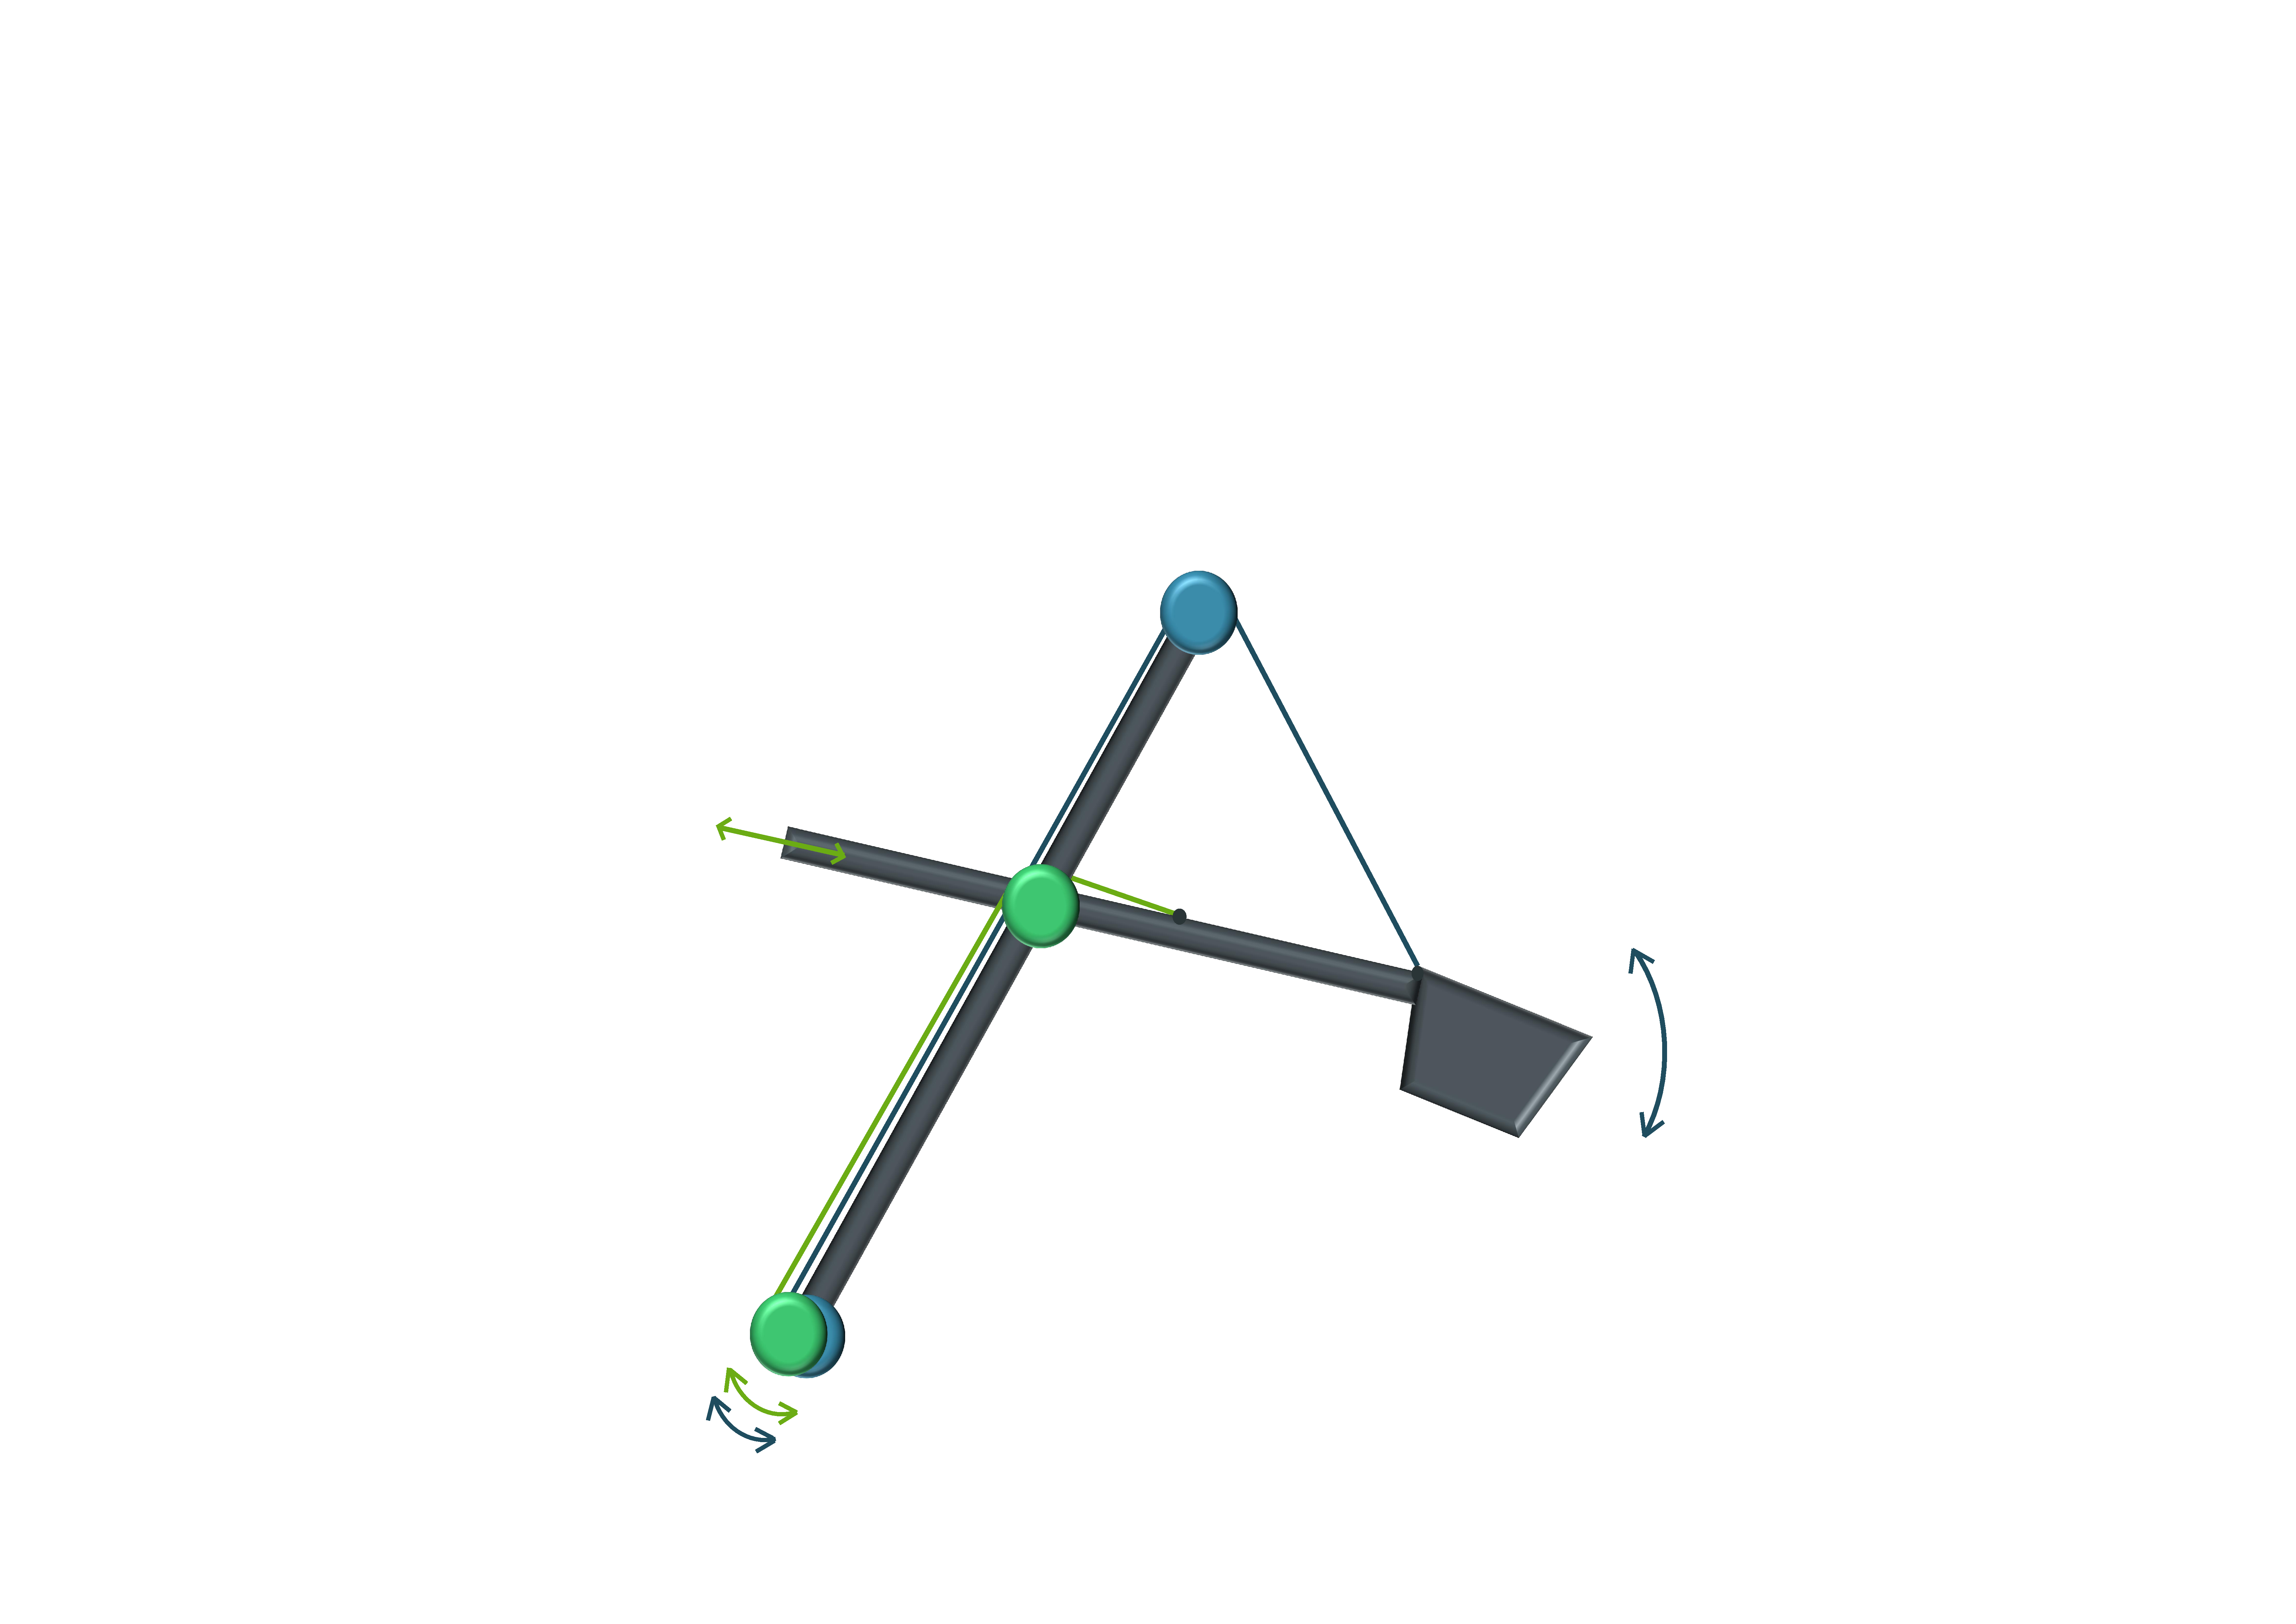
\includegraphics[trim=30cm 5cm 30cm 23cm, clip=true, width=\linewidth]{img/Excavator_Only}
		\column{.4\linewidth}
			\begin{itemize}
				\item{torque on cable reel}
				\item{friction of cable reel}
			\end{itemize}
	\end{columns}
\end{frame}

%\begin{frame}
	%\frametitle{Generalized Forces Q}
	%
	%Example: force at $A_2$:
	%\begin{align*}
	  %&F_{A_2} = \left[ \frac{\tau_{B_2}}{r_{B_2}} - \mu_{B_2} 
	  %\frac{\dot{s}}{r_{B_2}} - \mu_{P_2} \frac{\dot{s}}{r_{P_2}} \right]
	  %\left(
	  %\begin{matrix}
	    %\cos(\theta) \\
	    %\sin(\theta) \\
	  %\end{matrix}
	  %\right) \\
	%\end{align*}
	%
	%all generalized forces:
	%\begin{align*}
	  %&Q_s = \left( \frac{\partial r_{A_1}}{\partial s} \right)^T F_{A_1} 
	  %+ \left( \frac{\partial r_{A_2}}{\partial s} \right)^T F_{A_2} \\
	  %&Q_{\theta} = \left( \frac{\partial r_{A_1}}{\partial \theta} 
	  %\right)^T F_{A_1} + \left( \frac{\partial r_{A_2}}{\partial \theta} 
	  %\right)^T F_{A_2} \\
	%\end{align*}
%\end{frame}

%\begin{frame}
	%\frametitle{Parameters}
	%
	%\begin{tabular}{ll}
	  %& \\
	  %masses & $M_1$, $M_2$ \\
	  %&\\
	  %inertia of pulleys & $I_{B_1}$, $I_{B_2}$, $I_{P_1}$, $I_{P_2}$ \\
	  %&\\
	  %friction coefficients & $\mu_{B_1}$, $\mu_{B_2}$, $\mu_{P_1}$, 
	  %$\mu_{P_2}$  \\
	%\end{tabular}
%\end{frame}

\begin{frame}
	\frametitle{Lagrange Formalism}
	
	\begin{align*}
	  &\frac{d}{dt}\left(\frac{\partial T}{\partial \dot{s}}\right) -
	  \frac{\partial T}{\partial s} +
	  \frac{\partial V}{\partial s}
	  = Q_s \\
	  &{}\\
	  &\frac{d}{dt}\left(\frac{\partial T}{\partial \dot{\theta}}\right) -
	  \frac{\partial T}{\partial \theta} +
	  \frac{\partial V}{\partial \theta}
	  = Q_{\theta} \\
	\end{align*}
\end{frame}

\begin{frame}[c]
	\frametitle{Resulting ODE}
	
	Second order ODE from Lagrange Formalism:
	\begin{align*}
	  &A(x,p)
	  \begin{pmatrix} 
	    \ddot{s} \\ \ddot{\theta} \\
	  \end{pmatrix}
	  = b(x,u,p)
	\end{align*}
	
	Transformed into first order ODE:
	\begin{align*}
	  &\frac{d}{dt}
	  \begin{pmatrix}
	  s \\ \theta \\ \dot{s} \\ \dot{\theta}
	  \end{pmatrix}
	  =
	  \begin{pmatrix}
	    \dot{s} \\ \dot{\theta} \\ A^{-1}(x,p)b(x,u,p) \\
	  \end{pmatrix} 
	  = f(x,u,p) \\
	\end{align*}
	
	\vspace{-1.0cm}
	
	\begin{tabular}{ll}
	  & \\
	  state & $ x = (s,\theta,\dot{s},\dot{\theta})^T $ \\
	  control & $ u = (\tau_1,\tau_2)^T $ \\
	  parameters & $ p = (p_1,...,p_k)^T $ \\
	\end{tabular}
\end{frame}

\begin{frame}
	\frametitle{Discretization of the ODE}
	
	%Discretize time interval:
	%\begin{align*}
	  %&[0,T] = [t_0,t_1] \cup \ldots \cup [t_{m-1},t_m] \\
	%\end{align*}
	
	Discretize time interval:
	\begin{align*}
	  &[0,T] \rightarrow \left\{ 0=t_0, t_1, \dots, t_{m-1}, t_{m}=T 
\right\} \\
	\end{align*}
	
	Discretize state and control:
	\begin{align*}
	  &x_n = x(t_n) \\
	  &u_n = u(t_n) \\
	\end{align*}
	
\end{frame}

\begin{frame}
	
	\frametitle{Discretization of the ODE}
	
% 	Solve ODE for every time step $h_n=t_{n+1}-t_n$ (Explicit Euler):
	Explicit Euler for every time step $h_n=t_{n+1}-t_n$:
	\begin{align*}
	  &x_{n+1} \approx \tilde{x}_{n+1} = x_n + h_n f(x_n,u_n,p) \\
	\end{align*}
	
	Discrete constraint:
	\begin{align*}
	  &0 = x_{n+1} - \tilde{x}_{n+1} \quad \forall n = 0,\ldots,m-1
	\end{align*}

	
\end{frame}

\begin{frame}
	\frametitle{Discretization of the ODE}
	
	\begin{figure}[bth]
	  \begin{center}
	    %left, bottom, right, top
	    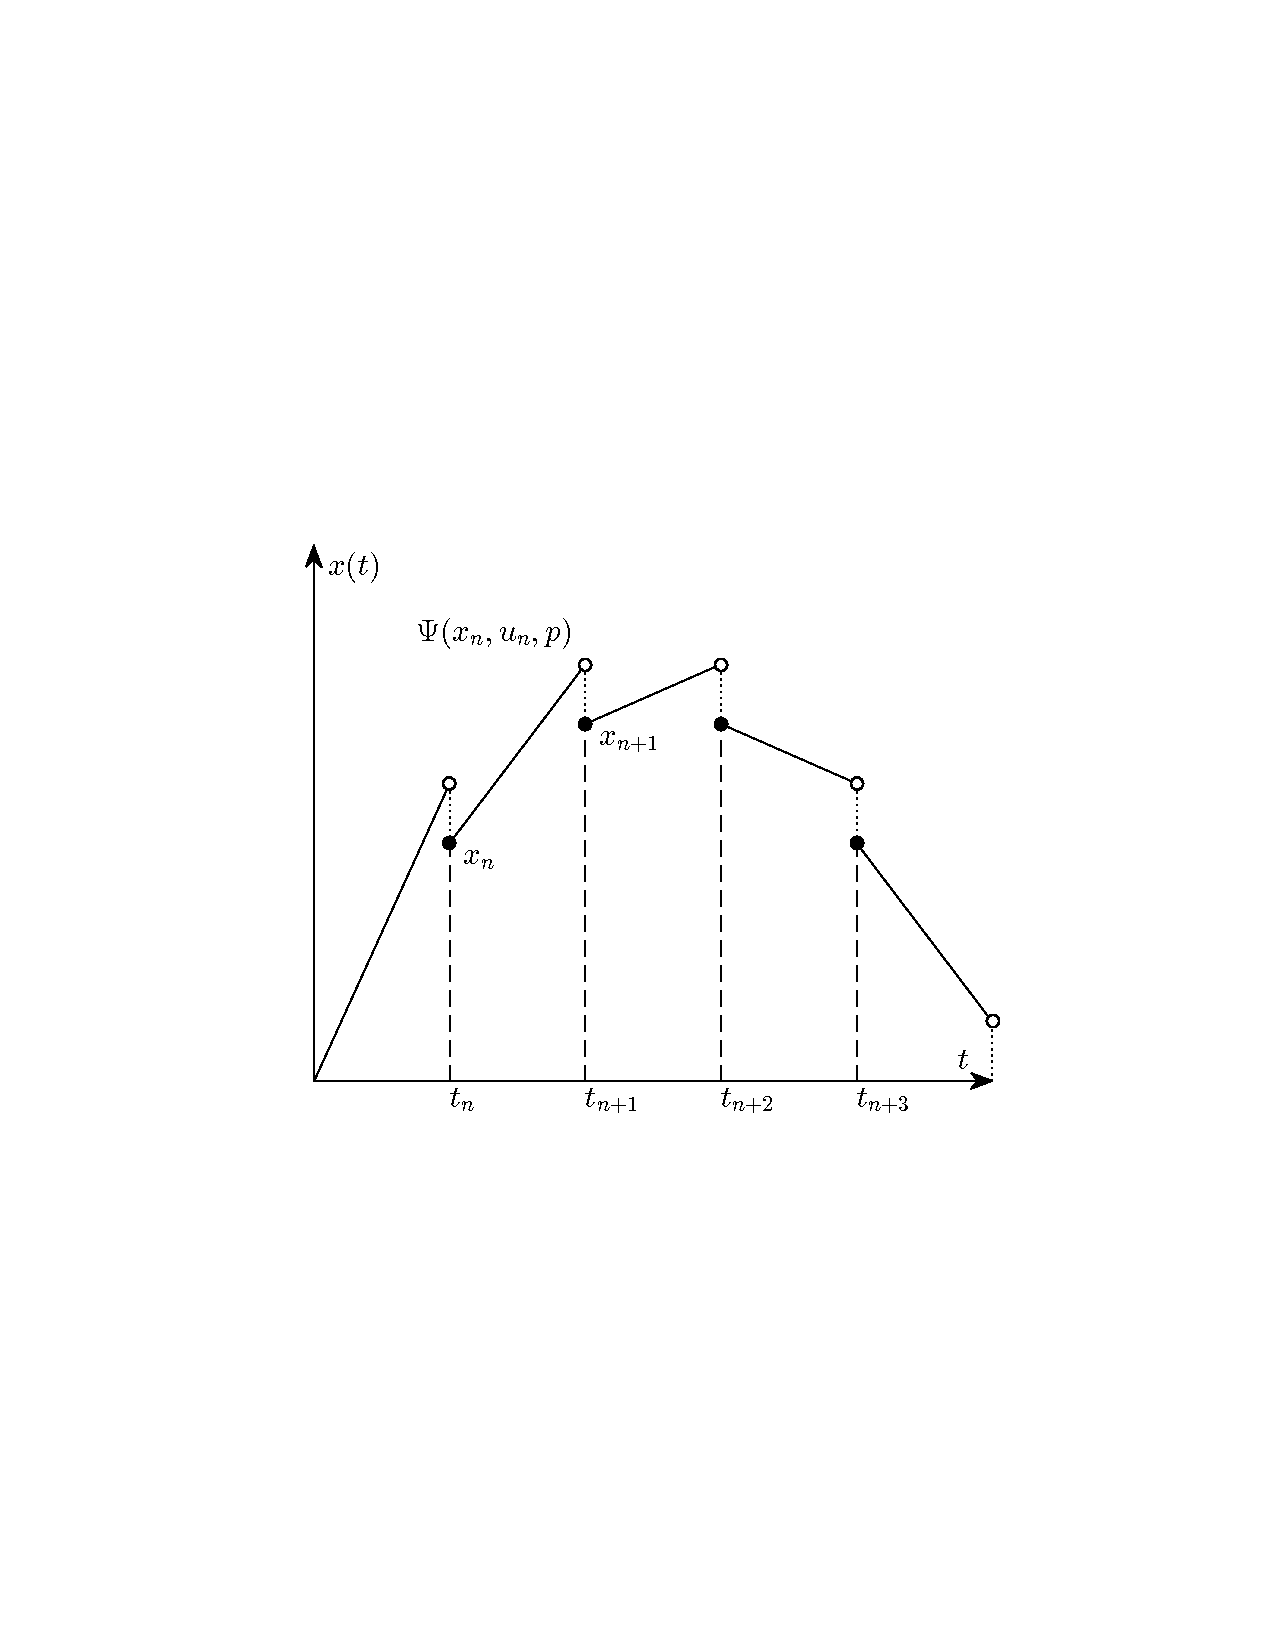
\includegraphics[trim=1cm 5cm 0cm 8cm, clip=true, 
	    width=\linewidth]{img/multShootPlot}
	  \end{center}
	\end{figure}
\end{frame}




%\section{Visualization}

\begin{frame}[c]
	\frametitle{Visualization}
	\begin{itemize}
		\item{MatLab/Simulink}
		\vspace{0.5cm}
		\item{verification of system's behaviors by simulating the motions for characteristic inputs}
	\end{itemize}
\end{frame}


\section{Parameter Identification: Physical Model}

\begin{frame}
	\frametitle{Discretization of the ODE}
	
	Discretize time interval:
	\begin{align*}
	  &[0,T] \rightarrow \left\{ 0=t_0, t_1, \dots, t_{m-1}, t_{m}=T 
\right\} \\
	\end{align*}
	
	Discretize state and control:
	\begin{align*}
	  &x_n = x(t_n) \\
   &u_n = u(t_n) \\
	\end{align*}
	
\end{frame}

\begin{frame}
	
	\frametitle{Discretization of the ODE}
	
% 	Solve ODE for every time step $h_n=t_{n+1}-t_n$ (Explicit Euler):
	Explicit Euler for every time step $h_n=t_{n+1}-t_n$:
	\begin{align*}
        &\Psi(x_n,u_n,p) = x_n + h_n f(x_n,u_n,p)  \\
	\end{align*}
	
	Discrete constraint:
	\begin{align*}
        &0 = x_{n+1} - \Psi(x_n,u_n,p) =: \Phi_n(x,u,p) \quad \forall n = 0,\ldots,m-1
	\end{align*}

	
\end{frame}

\begin{frame}
	\frametitle{Discretization of the ODE}
	
	\begin{figure}[bth]
	  \begin{center}
	    %left, bottom, right, top
	    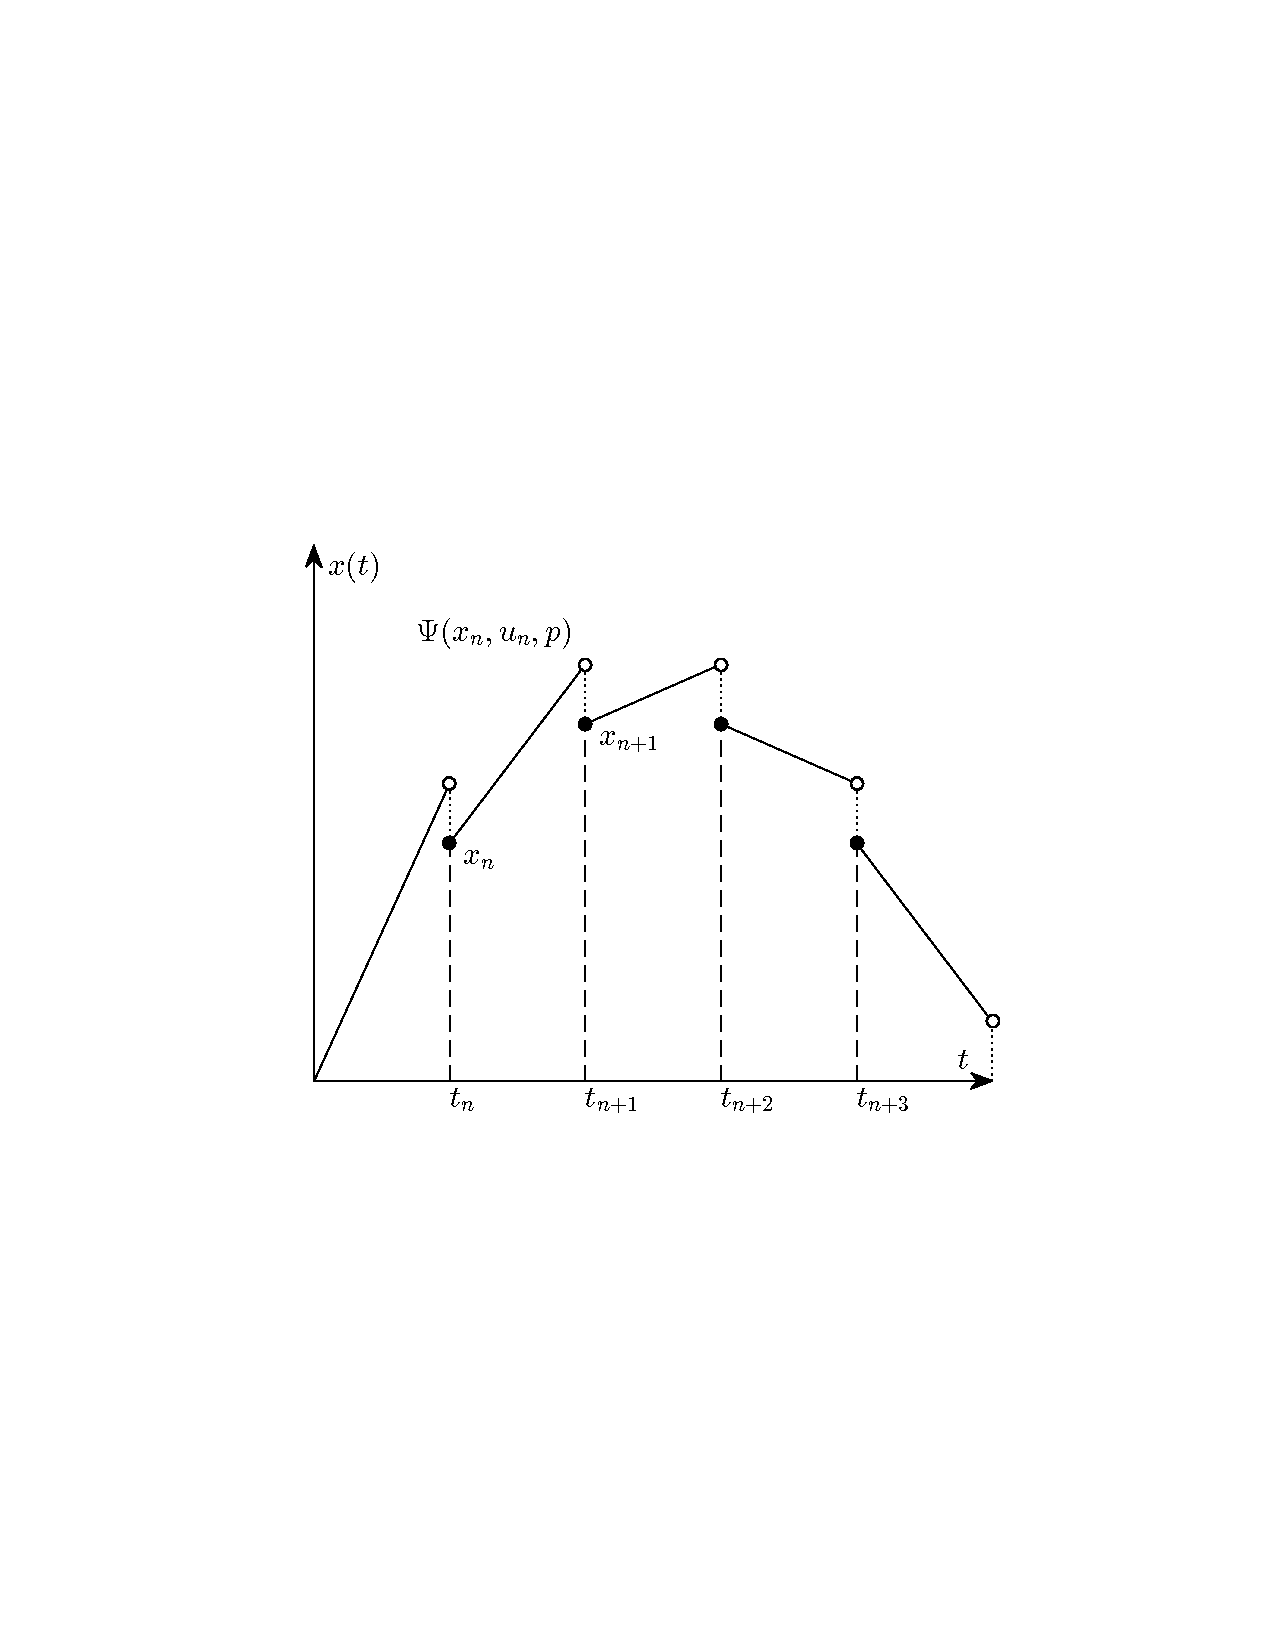
\includegraphics[trim=1cm 5cm 0cm 8cm, clip=true, width=\linewidth]{img/multShootPlot}
	  \end{center}
	\end{figure}
\end{frame}





\begin{frame}
    \frametitle{Problem Setting}
	\begin{columns}
	    
    
    \begin{column}{0.5\textwidth}
    Given:
    \begin{itemize}
        \item{control $\bar{u}$}
        \item{motion $\bar{x}$ related to $\bar{u}$ and $\bar{p}$}
    \end{itemize}

    Unknown:
    \begin{itemize}
        \item{parameters $\bar{p}$ of the excavator}
    \end{itemize}

    Output:
    \begin{itemize}
        \item{parameters $p$}
    \end{itemize}
    \end{column}
    
    \begin{column}{0.4\textwidth}

\includemedia[
  label      = DD,
  width      = 50mm,
  height     = 50mm,
  activate   = pageopen,
  addresource= videos/traj_x_ref3.mp4,
  flashvars={flv=videos/traj_x_ref3.mp4 & autoplay=1 & loop =1}
]{}{player_flv_maxi.swf}

\end{column}    
    
    
    
    \end{columns}
\end{frame}

\begin{frame}
    \frametitle{Problem Formulation}
    Natural approach: Optimal Control Problem
    \begin{align*}
        \min_{x,p} & & \frac{1}{2} \| \bar{x} - x \|^2 & & \\
        \operatorname{s.t.} & & \Phi(x,\bar{u},p) & = 0 & & \\
                            & & p & \geq 0 & & \\
    \end{align*}

    \begin{tabular}{ll}
        state & $ x = (s,\theta,\dot{s},\dot{\theta})^T $ \\
        parameters & $ p = (p_1,...,p_k)^T $ \\
        control & $ \bar{u} = (\tau_1,\tau_2)^T $ \\
        desired motion & $\bar{x}$ \\
    \end{tabular}
\end{frame}

%\begin{frame}
%    \frametitle{Problem Formulation}
%    \onslide<1->
%    Input:
%    \begin{itemize}
%        \item{control $\bar{u}$}
%        \item{desired motion $\bar{x}$ related to $\bar{u}$}
%    \end{itemize}
%
%    \onslide<2->
%    Output:
%    \begin{itemize}
%        \item{parameters $p$ of the excavator}
%        \item{x, but not of interest}
%    \end{itemize}
%
%    \onslide<3>
%    Idea:
%    \begin{itemize}
%        \item{get rid of variable $x$}
%        \item{set $x := \bar{x}$}
%        \item{solve a relaxed problem}
%    \end{itemize}
%\end{frame}

\begin{frame}
    \frametitle{Problem Formulation}

    \onslide<1->
    Original Problem
    \begin{align*}
        \min_{x,p} & & \frac{1}{2} \| \bar{x} - x \|^2 & & \\
        \operatorname{s.t.} & & \Phi(x,\bar{u},p) & = 0 & & \\
                            & & p & \geq 0 & & \\
    \end{align*}

    \onslide<2->
    Set $x \leftarrow \bar{x}$

    \onslide<3>
    Reinterpreted Problem
    \begin{align*}
        \min_{p}  & & \frac{1}{2} \| \Phi(\bar{x},\bar{u},p) \|^2 & & \\
        \operatorname{s.t.} & & p & \geq 0 & & \\
    \end{align*}
\end{frame}

\begin{frame}
    \begin{align*}
        \min_{p}  & & \frac{1}{2} \| \Phi(\bar{x},\bar{u},p) \|^2 & & \\
        \operatorname{s.t.} & & p & \geq 0 & & \\
    \end{align*}
    %\begin{align*}
    %    & \Phi_n(x,\bar{u},p) = x_{n+1} - \Psi(x_n,\bar{u}_n,p)   \quad \forall n = 0,\ldots,m-1 \\
    %\end{align*}
    \begin{itemize}
        \item{$\bar{x}$ solves ODE for $\bar{p}$}
        \item{$\Phi(\bar{x},\bar{u},\bar{p}) \rightarrow 0$ for discretization $m \rightarrow \infty$}
        \item{number of parameters fix}
    \end{itemize}
\end{frame}

\begin{frame}
    \frametitle{Comparison of the Approaches}

    \begin{columns}[t]
        \column{.5\linewidth}
            \begin{figure}
                \centering
                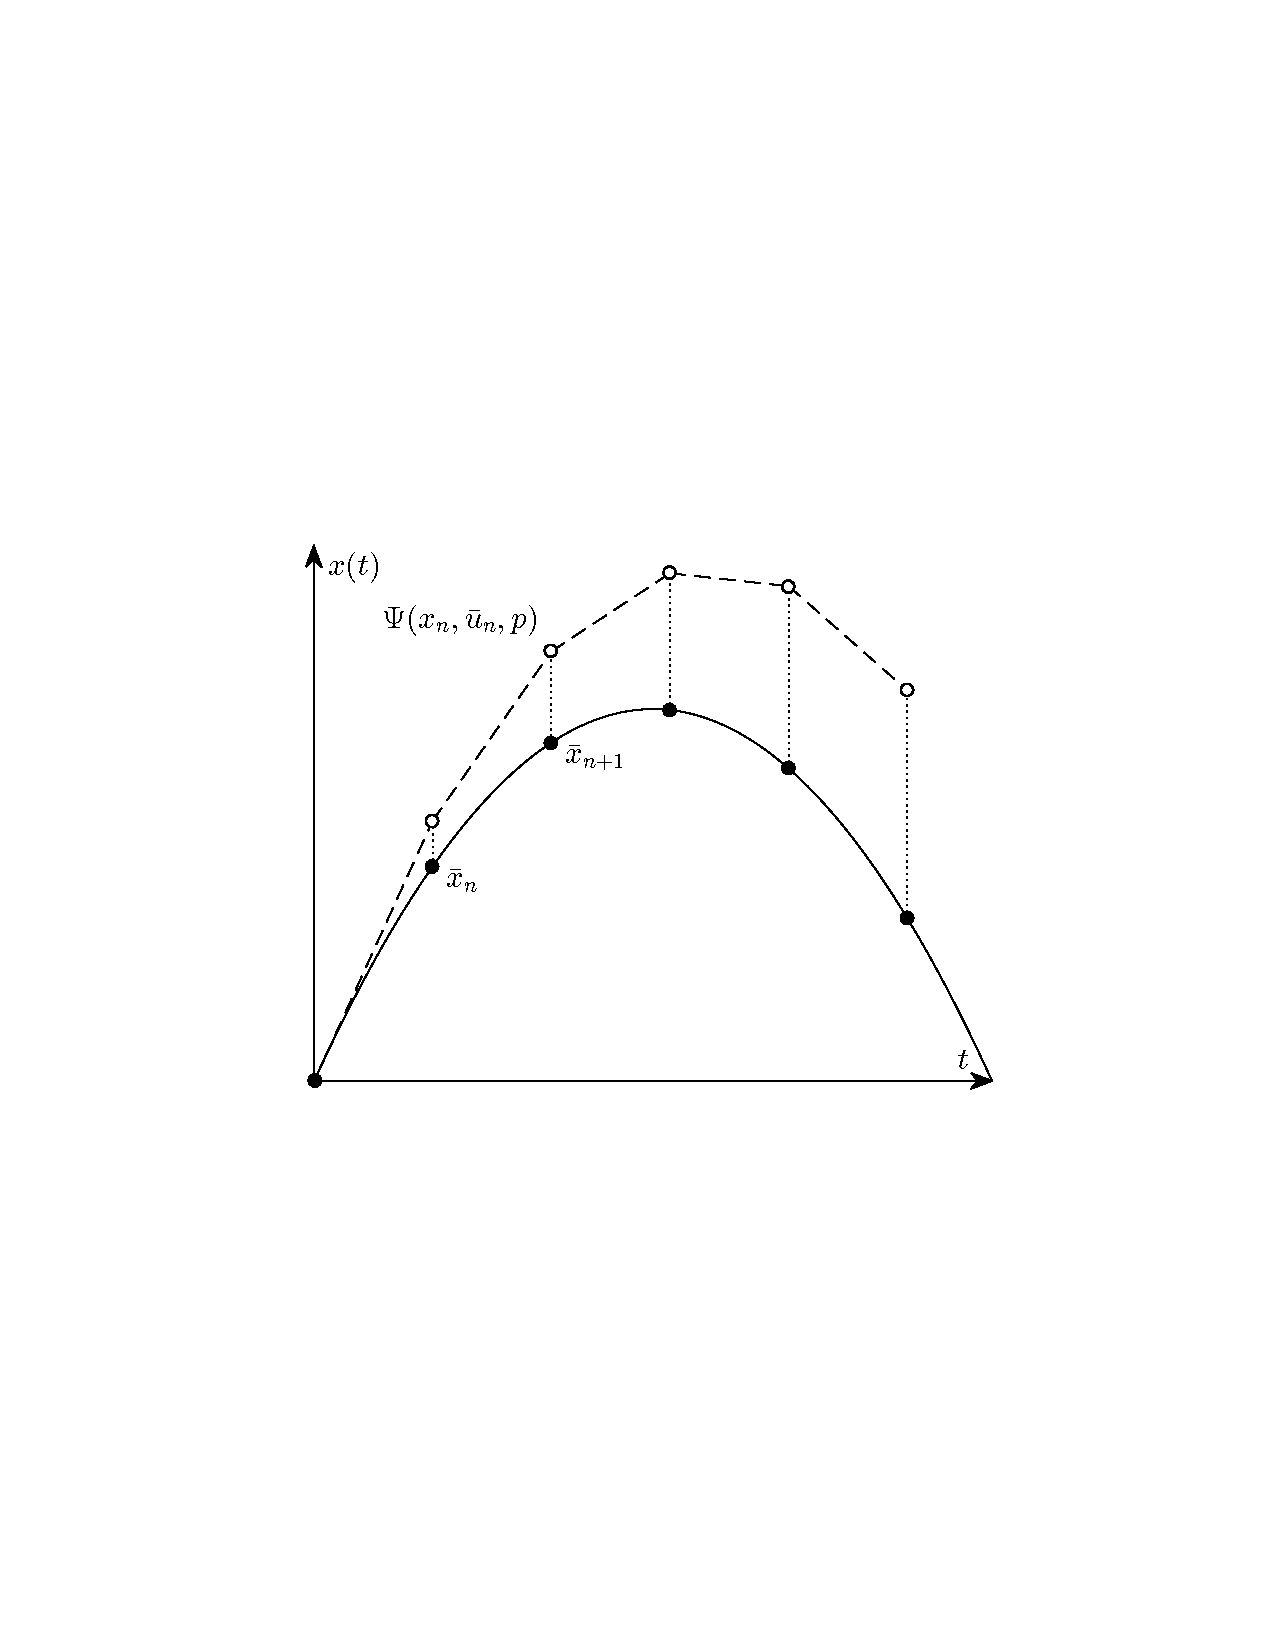
\includegraphics[trim=3cm 7cm 3cm 9cm, clip=true, width=\linewidth]{img/contExplEulerPlot}
            \end{figure}
        \column{.5\linewidth}
            \begin{figure}
                \centering
                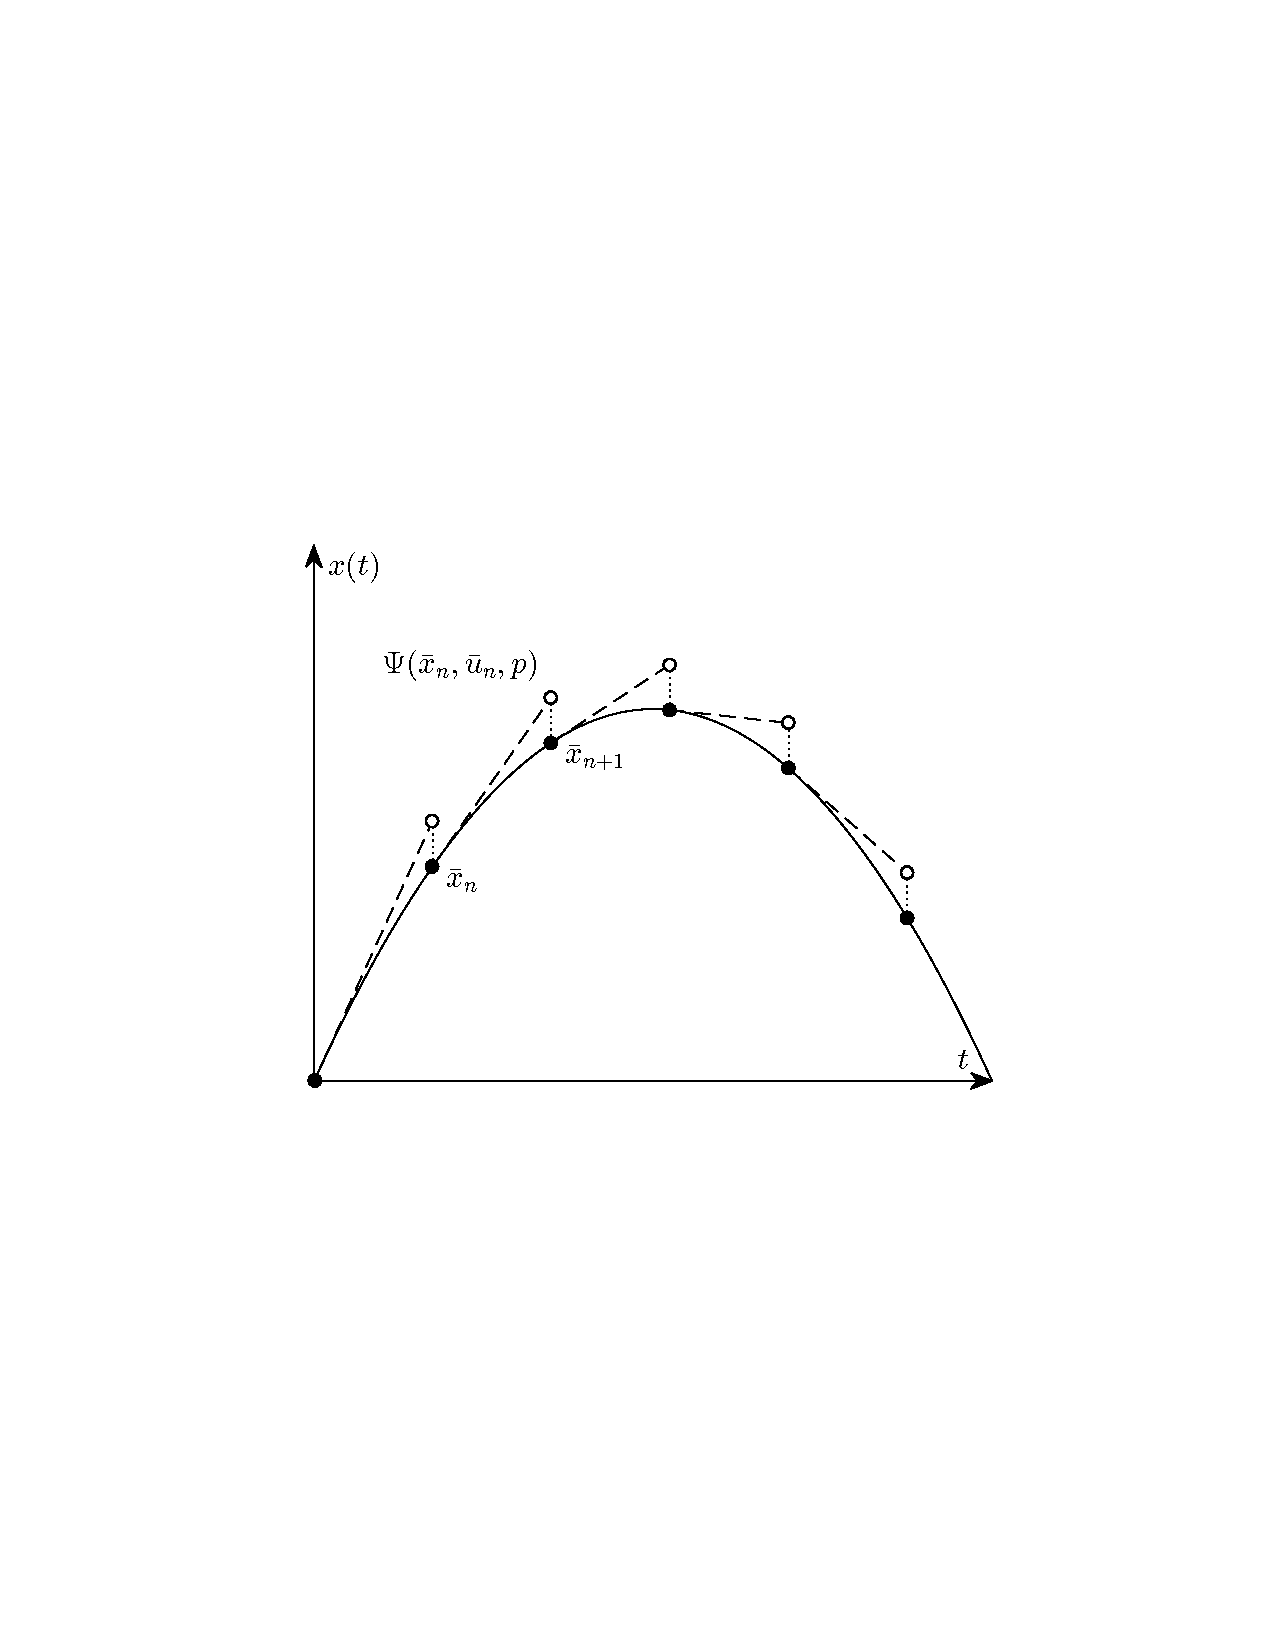
\includegraphics[trim=3cm 7cm 3cm 9cm, clip=true, width=\linewidth]{img/stepExplEulerPlot}
            \end{figure}
    \end{columns}
    \begin{center}
        continuous vs. stepwise Approximation
    \end{center}
\end{frame}

\begin{frame}
    \frametitle{Example Instance}
    \begin{itemize}
        \item{$[0,T] = [0,14s]$}
        \item{1500 time steps}
        \item{$p_0 \in [0.8  \bar{p}, 1.2  \bar{p}]$}
        \item{$x(p)$ solution of ODE for given $p$}
        \item{internally 5 trajectories in parallel}
    \end{itemize}

\end{frame}

\begin{frame}
    \frametitle{Results}
    \begin{columns}[t]
        \column{.5\linewidth}
            \begin{figure}
                \centering
                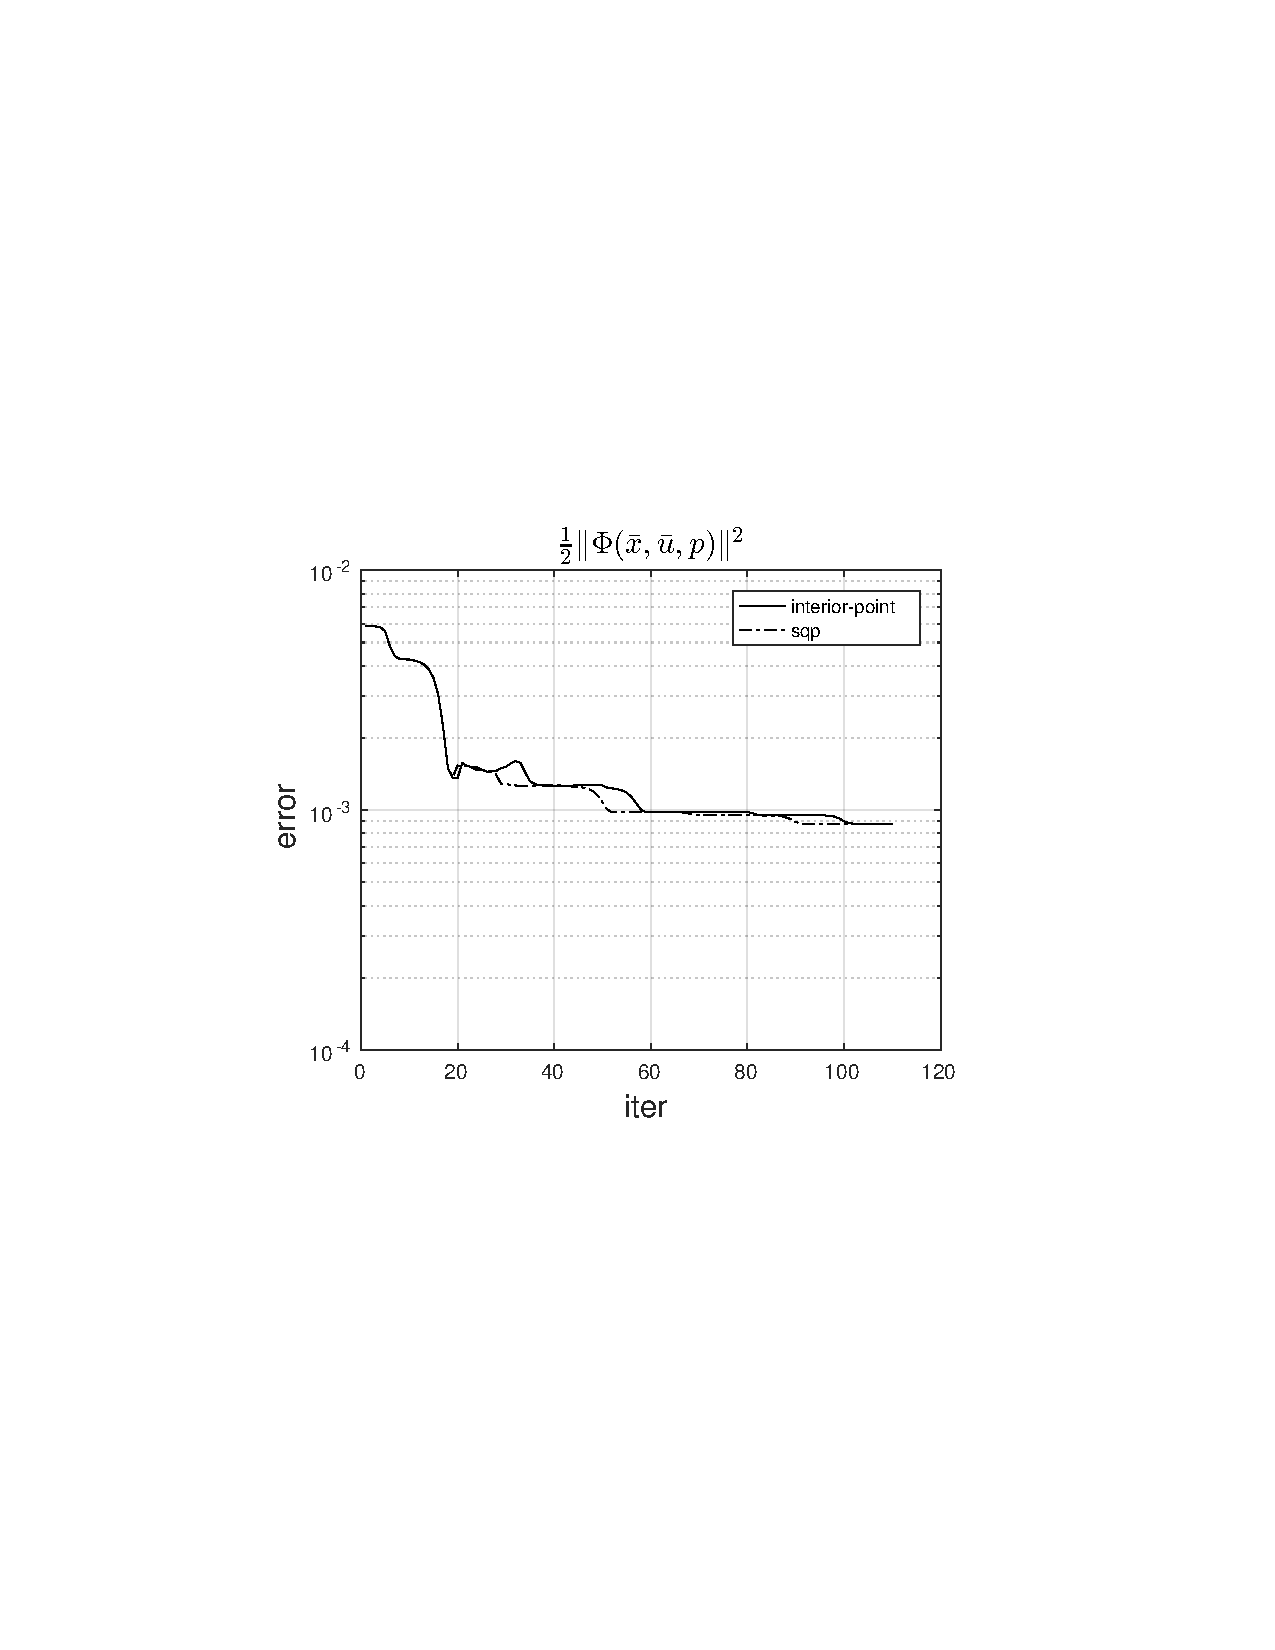
\includegraphics[trim=4cm 9cm 4cm 8.5cm, clip=true, width=\linewidth]{img/convPlotPhi}
            \end{figure}
        \column{.5\linewidth}
            \begin{figure}
                \centering
                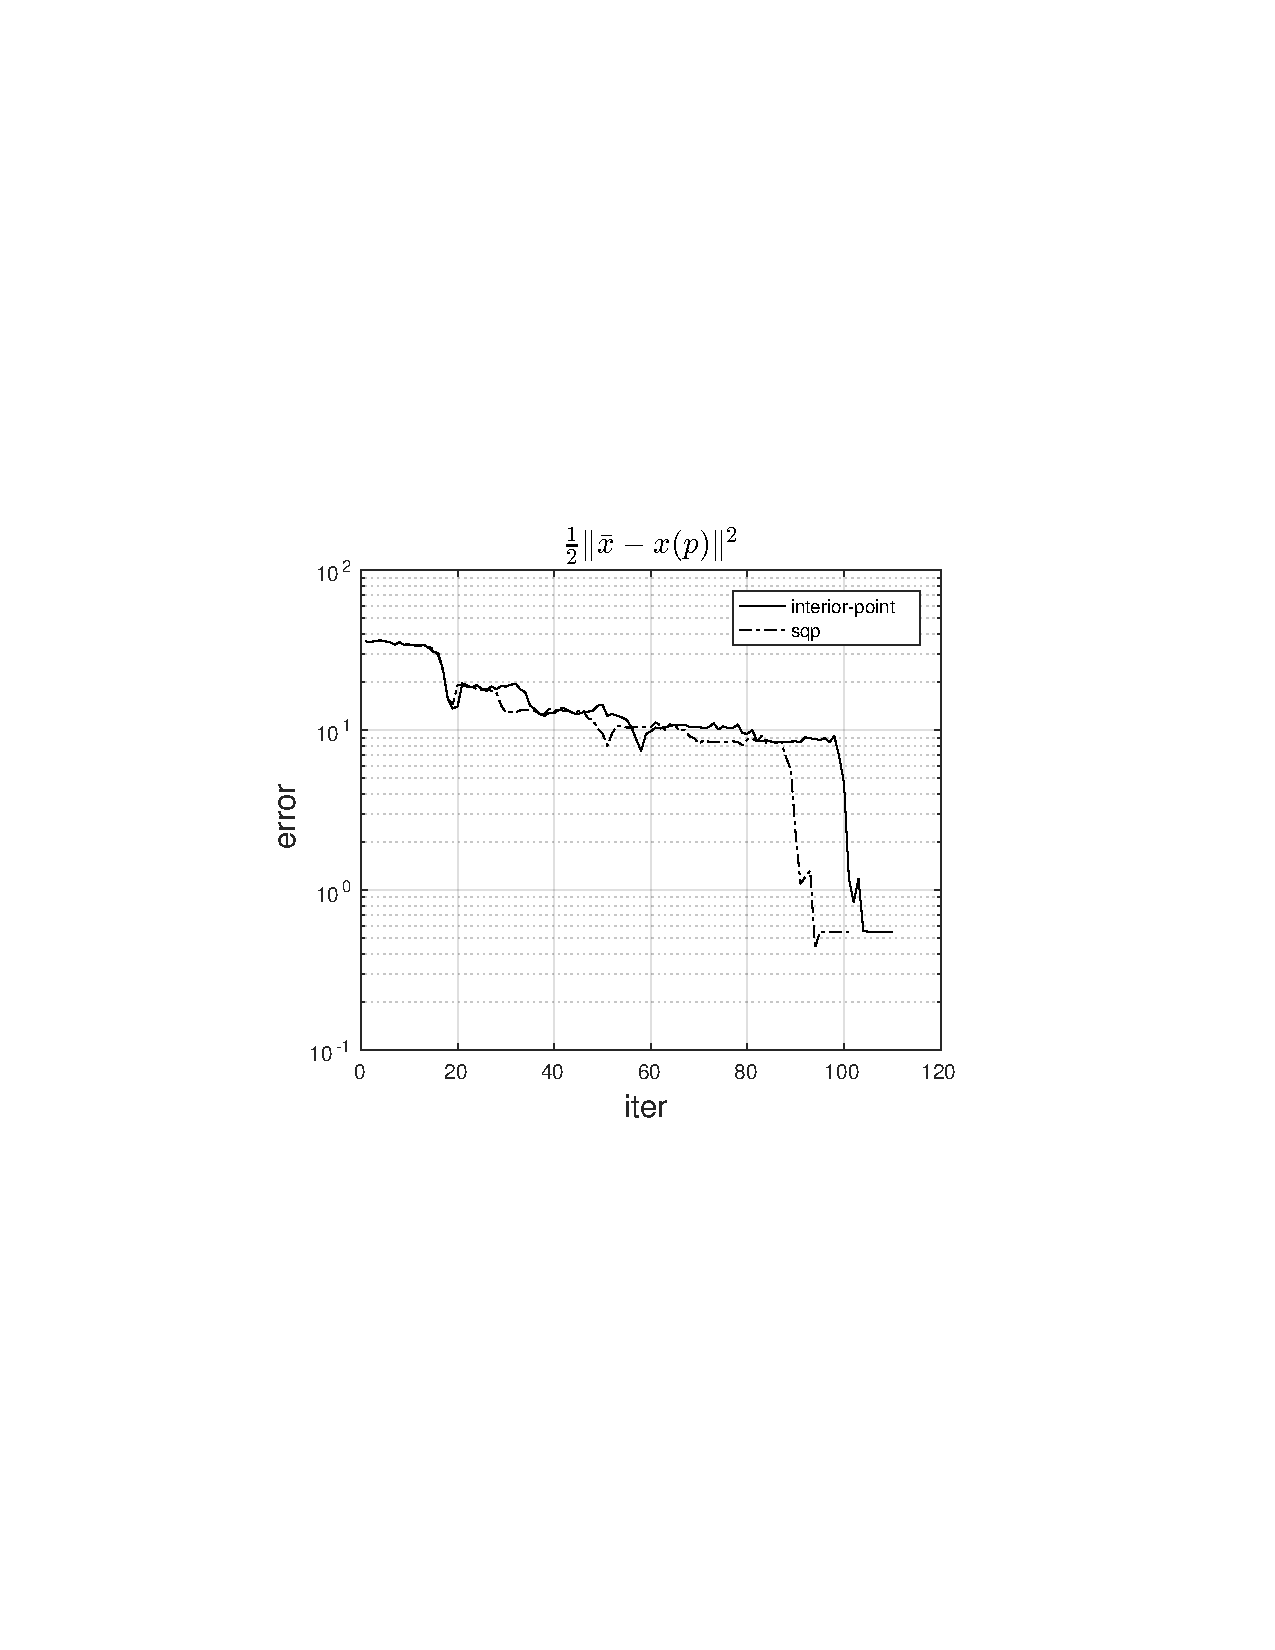
\includegraphics[trim=4cm 9cm 4cm 8.5cm, clip=true, width=\linewidth]{img/convPlotX}
            \end{figure}
    \end{columns}
\end{frame}

\begin{frame}
    \frametitle{Results}

    \begin{columns}[t]
        \column{.5\linewidth}
            \begin{figure}
                \centering
                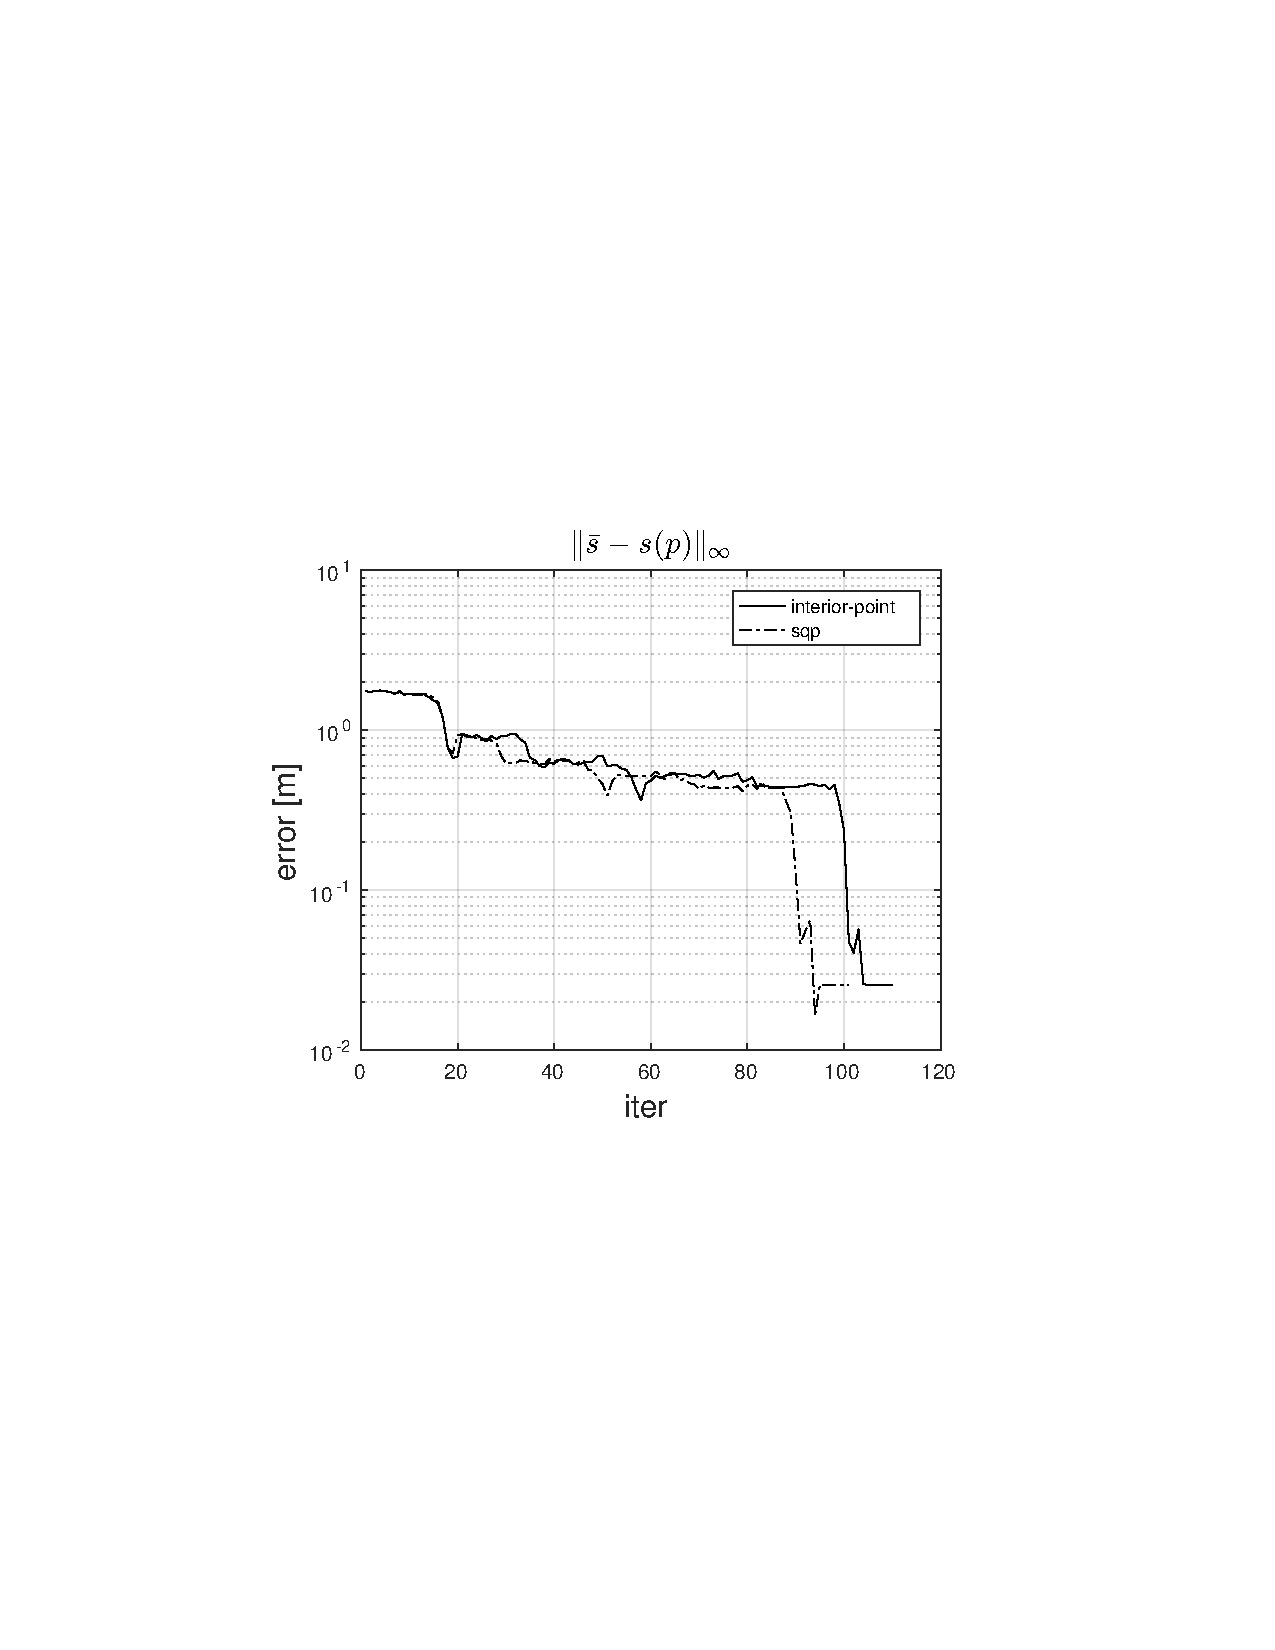
\includegraphics[trim=4cm 9cm 4cm 8.5cm, clip=true, width=\linewidth]{img/convPlotS}
            \end{figure}
        \column{.5\linewidth}
            \begin{figure}
                \centering
                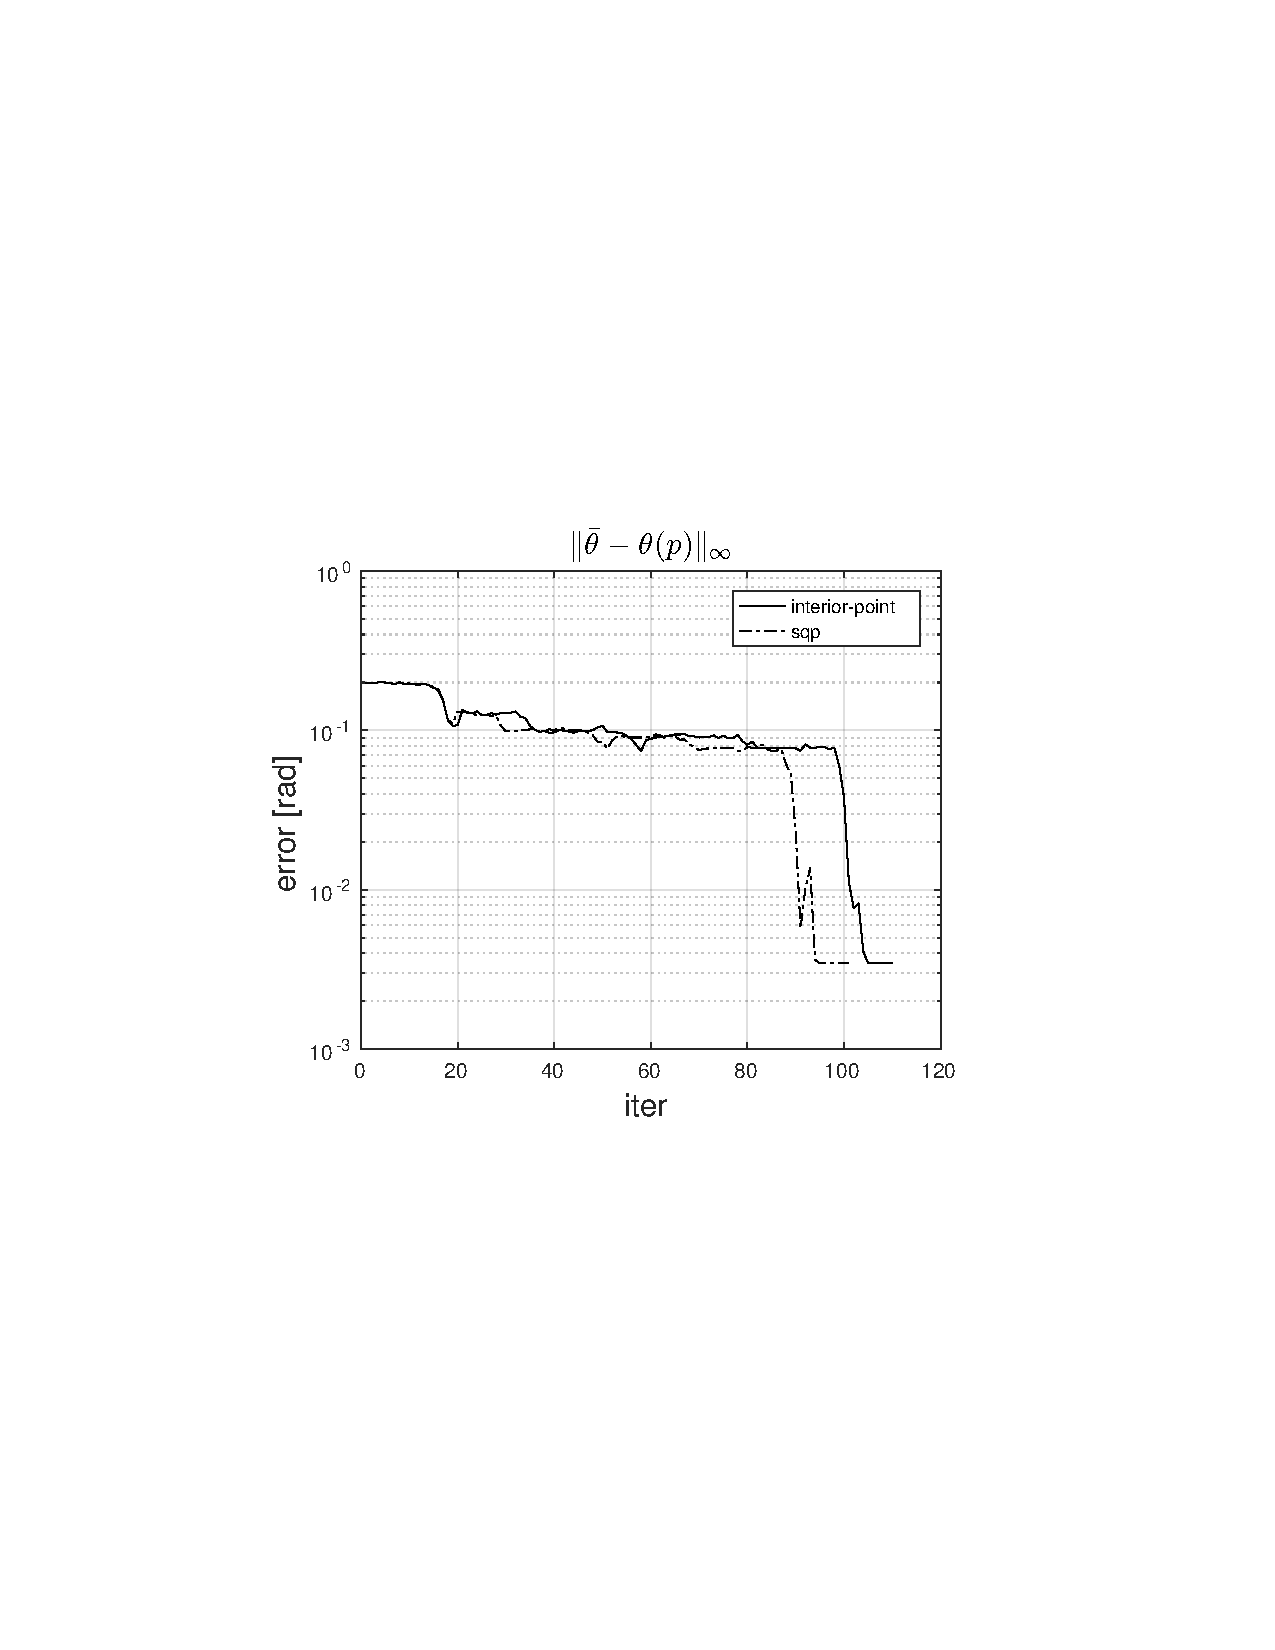
\includegraphics[trim=4cm 9cm 4cm 8.5cm, clip=true, width=\linewidth]{img/convPlotT}
            \end{figure}
    \end{columns}

    \begin{center}
        Exact up to $3\text{cm}$
    \end{center}
\end{frame}

\begin{frame}
    \frametitle{Results}
    \begin{columns}[t]
        \column{.5\linewidth}
            \begin{figure}
                \centering
                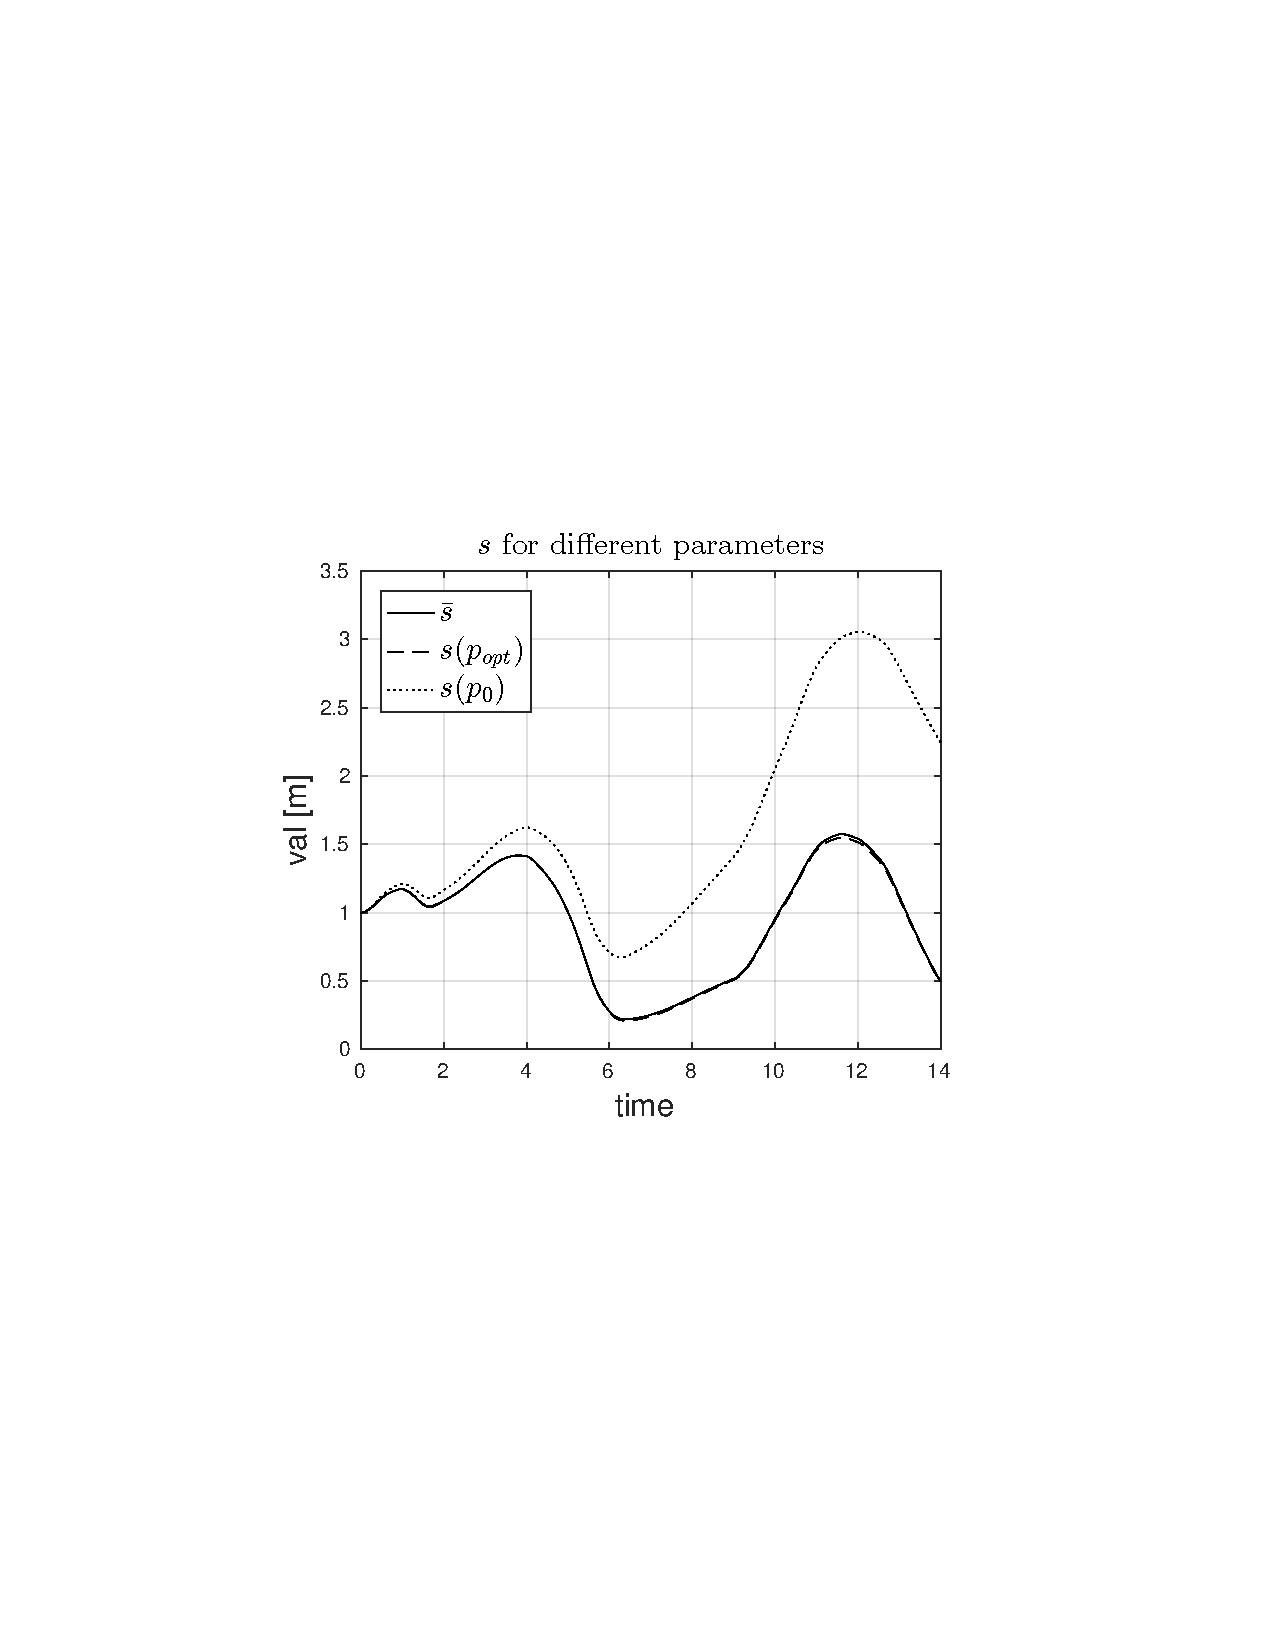
\includegraphics[trim=4cm 9cm 4cm 8.5cm, clip=true, width=\linewidth]{img/convPlotTrajS}
            \end{figure}
        \column{.5\linewidth}
            \begin{figure}
                \centering
                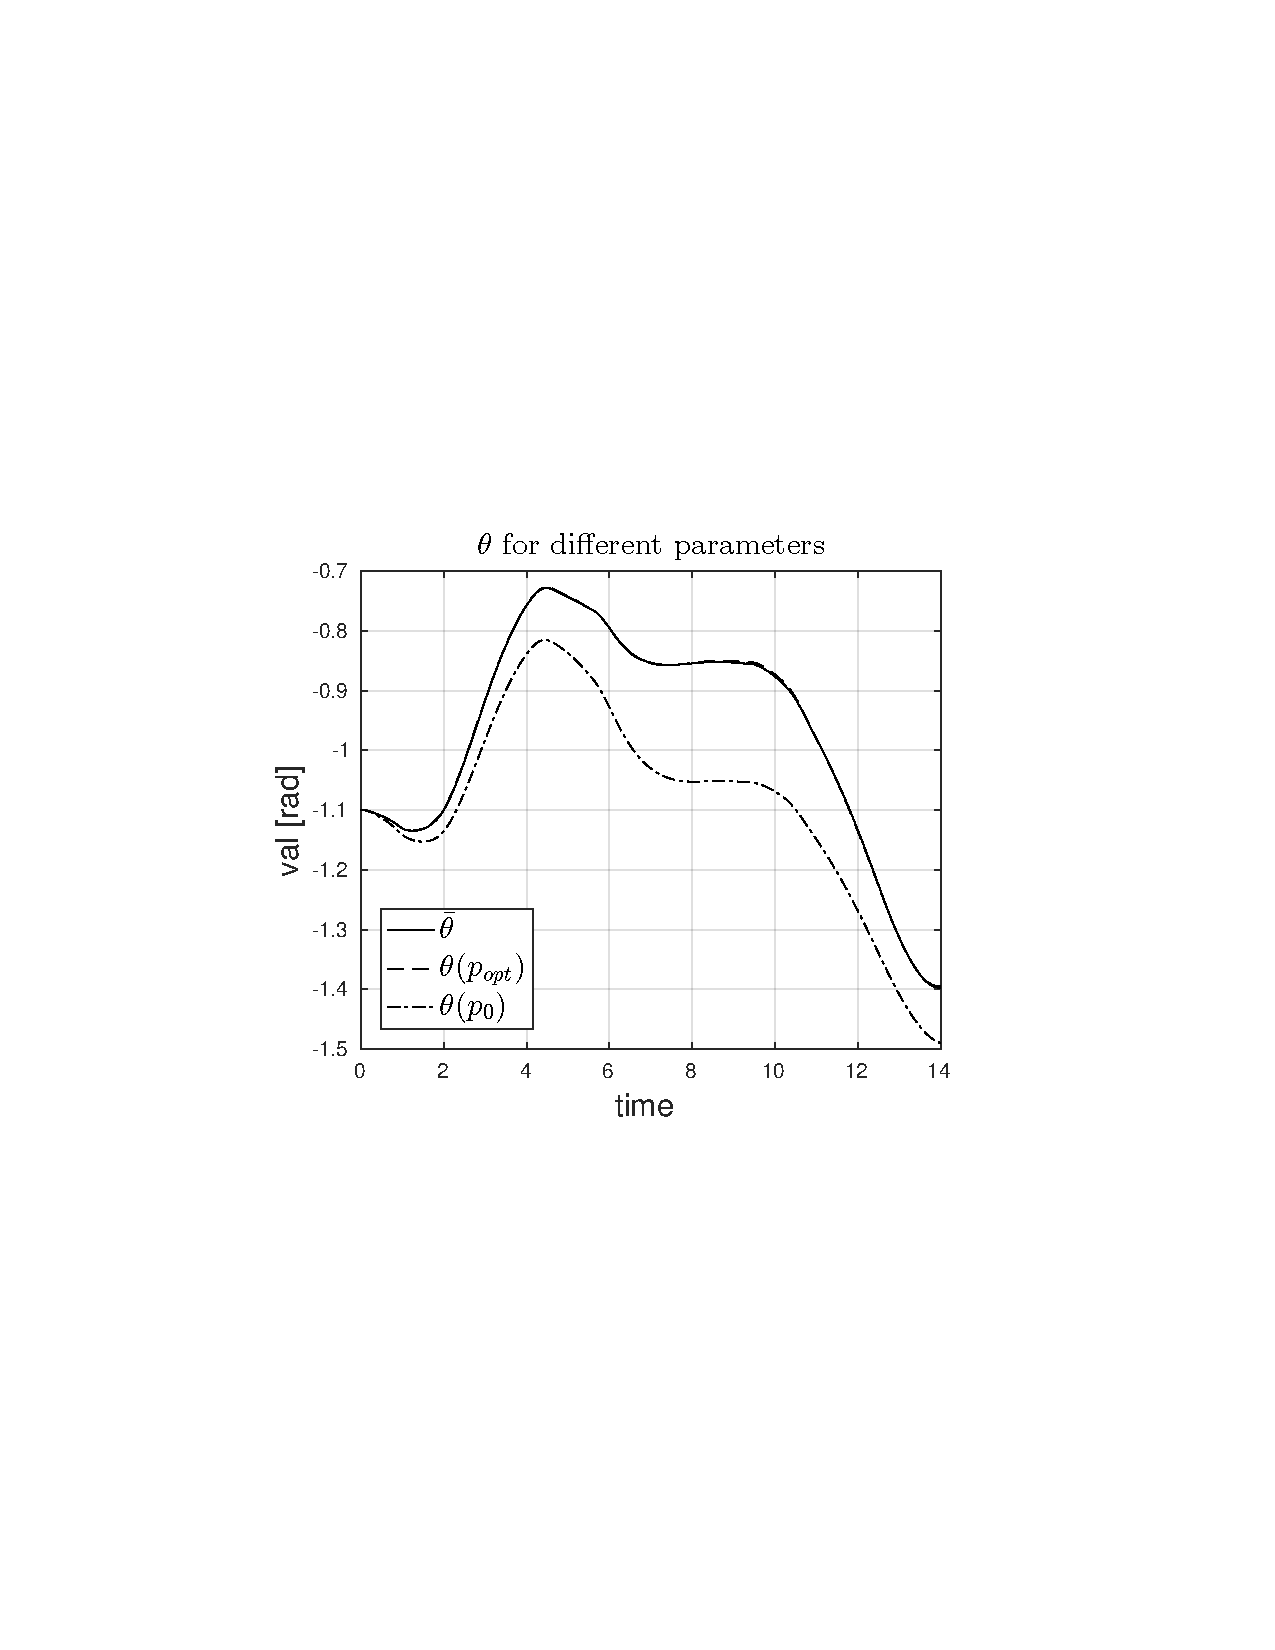
\includegraphics[trim=4cm 9cm 4cm 8.5cm, clip=true, width=\linewidth]{img/convPlotTrajT}
            \end{figure}
    \end{columns}
\end{frame}


\section{Parameter Optimization}

\begin{frame}[c]
\frametitle{Parameters}
Examples:
\begin{itemize}
	\item{Friction coefficients $\mu_{B_1}$, $\mu_{B_2}$, $\mu_{P_1}$, $\mu_{P_2}$}
	\item{masses $M_1$, $M_2$}
	\item{inertia $I_{B_1}$, $I_{B_2}$, $I_{P_1}$, $I_{P_2}$}
\end{itemize}
\vspace{0.5cm}
Why do we need parameter optimization?
\begin{itemize}
	\item{hard to measure}
	\item{may change over time}
\end{itemize}
\end{frame}

\begin{frame}[c]
\frametitle{Blackbox Model}
\begin{itemize}
	\item{contains a realistic model from Siemens}
	\item{confidential information}
\end{itemize}
\vspace{0.5cm}
tba
%\begin{columns}[t]
	%\column{.5\textwidth}
		%\textbf{Input}
		%\begin{itemize}
			%\item{control}
			%\item{parameters}
		%\end{itemize}
	%\column{.5\textwidth}
		%\textbf{Output}
		%\begin{itemize}
			%\item{motion}
		%\end{itemize}
%\end{columns}
\end{frame}

\begin{frame}
\frametitle{Parameter Optimization}
\begin{itemize}
	\item{black box $\Rightarrow$ derivative-free optimization}
	\vspace{0.5cm}
	\item{need own model for testing}
\end{itemize}
\end{frame}



%------------------------------------------------------------------------- Summary ---------------------------------------------------------------------------------------

\section{Summary}

\begin{frame}[c]
	\frametitle{Summary}

	\begin{columns}
		\onslide<1->
		\column{.5\linewidth}
			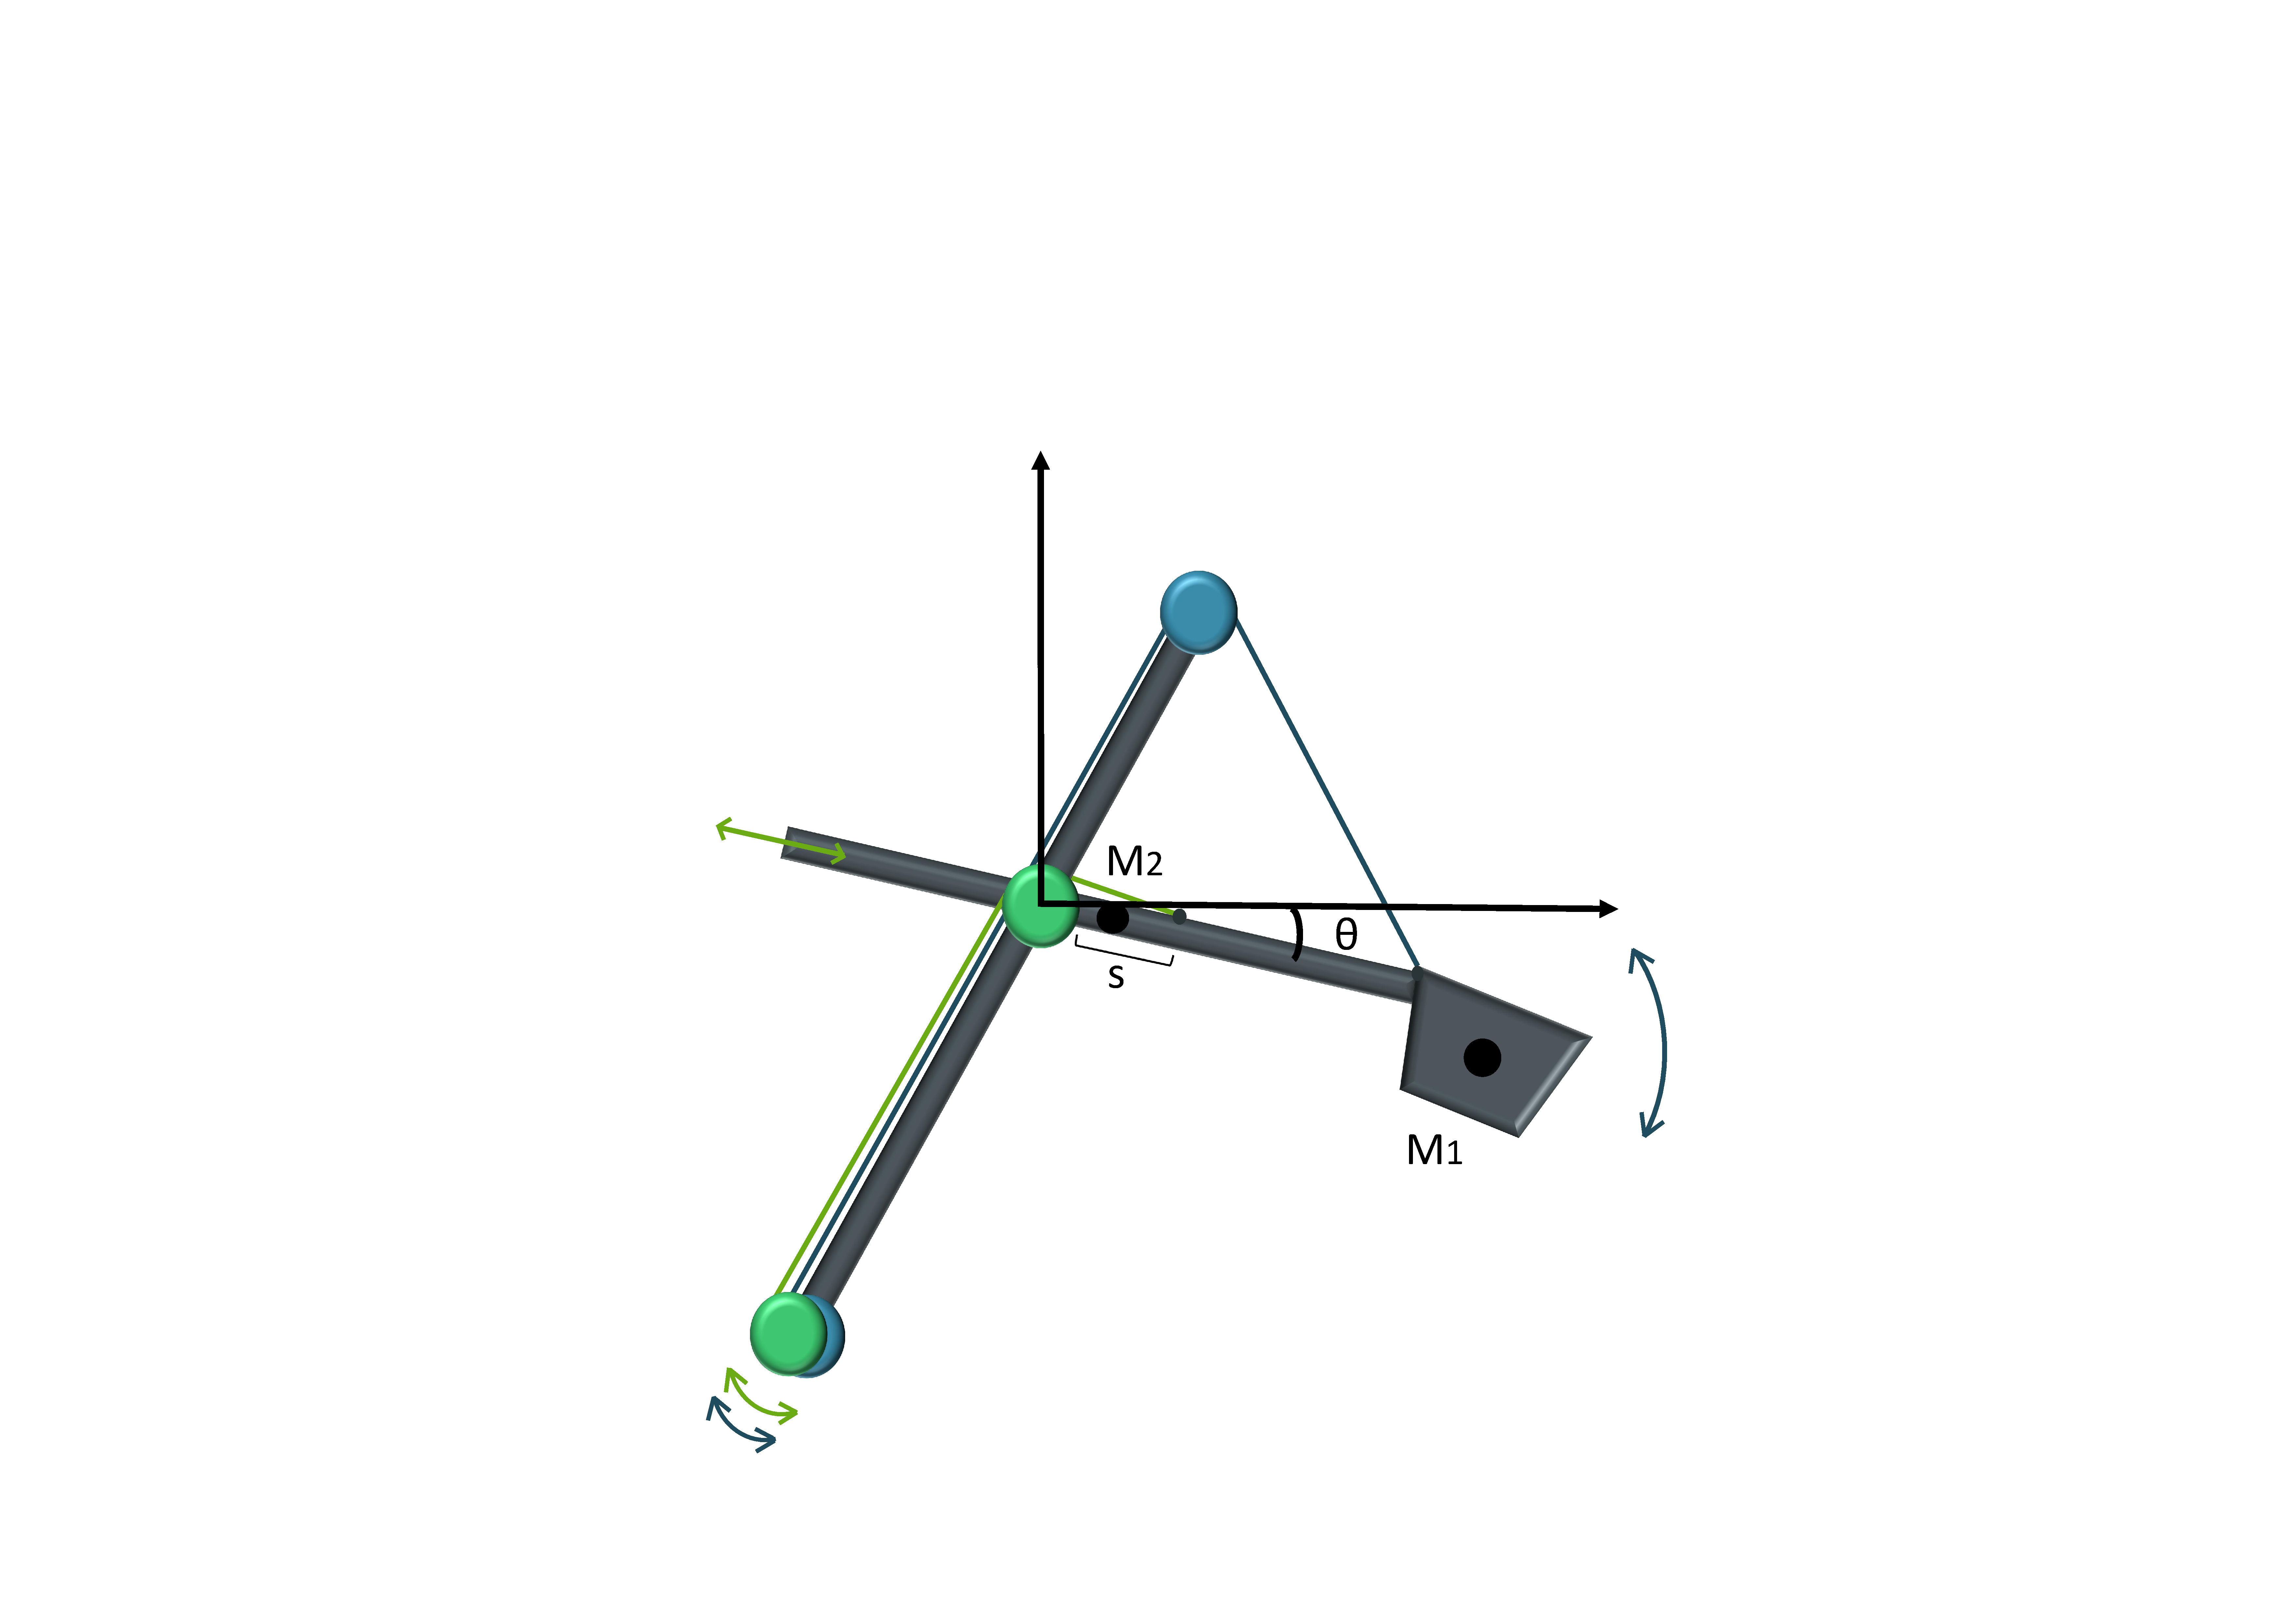
\includegraphics[trim=30cm 5cm 30cm 23cm, clip=true, width=\linewidth]{img/Excavator_results}
		
		\onslide<2>
		\column{.5\linewidth}
			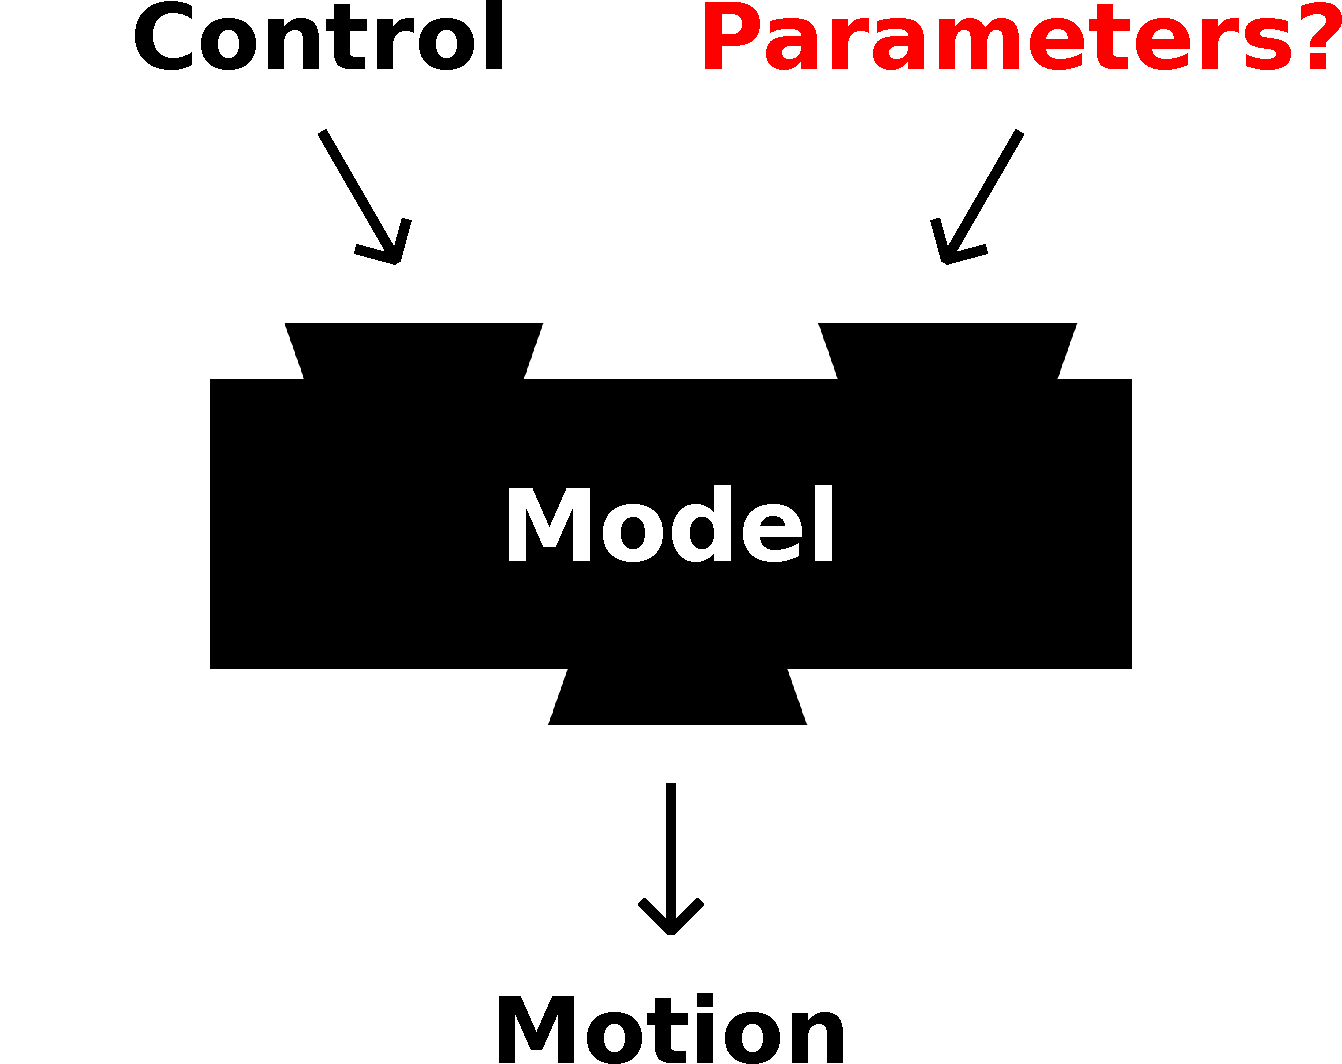
\includegraphics[width=\linewidth]{img/Blackbox_4}
	\end{columns}
\end{frame}

\end{document}

